\documentclass{cmspaper}
\usepackage{color}
\usepackage{graphicx}
\usepackage{wrapfig}
\usepackage{slashbox}
\usepackage{epstopdf}  %added for MAC compiler
\usepackage{pdfpages}
\usepackage{lineno}
\usepackage{verbatim}
\RequirePackage{lineno} 
%\RequirePackage{lineno} 

\usepackage{wrapfig}

%Note to authors: these definitions are suggested to be used for consistency
\newcommand{\pt}{$p_T$ }
\newcommand{\mll}{\ensuremath{M_{\ell\ell}}}
\newcommand{\z}{$Z$ }
\newcommand{\Z}{$Z$ } %redundancy can be good
\newcommand{\ttbar}{\ensuremath{t\bar{t}} }
\newcommand{\emu }{\ensuremath{e\mu}}
\newcommand{\ee  }{\ensuremath{ee}}
\newcommand{\eepm}{\ensuremath{e^+ e^-}}
\newcommand{\mm  }{\ensuremath{\mu\mu}}
\newcommand{\mmpm}{\ensuremath{\mu^+ \mu^-}}
\newcommand{\empm}{\ensuremath{e^\pm \mu^\mp}}
\newcommand{\ase}[2]{\ensuremath{_{~- #1}^{~+ #2}}}
\newcommand{\met}{\mbox{$\raisebox{.3ex}{$\not$}E_T$\hspace*{0.5ex}}} 
\newcommand{\effr}{$R_{e\mu}$} %used to be \epsilon
\newcommand{\sta}{$\sigma\times A$} %notation is such that A includes BR
\newcommand{\statistics}{CL$_\mathrm{S}$}

%The lumi so that if it changes it's easier to update
\newcommand{\lumi}{976~pb$^{-1}$}

%loose(tight) signal region met cut
\newcommand{\signalmetl}{100}
\newcommand{\signalmett}{200}

\newcommand{\resulttitle}
%{                      &   N(MET $>30$)  GeV    &   N(MET $>60$)  GeV    &   N(MET $>100$) GeV    &   N(MET $>200$) GeV \\}
{                       &   MET $>30$  GeV    &   MET $>60$  GeV    &   MET $>100$ GeV    &   MET $>200$ GeV \\}

%add this to captions (?)
%\newcommand{\oflw}{}

\begin{document}


\begin{titlepage}

  %\internalnote{2011/000}
  \cmsnote{2011/000}

  \date{\today}
 
  \title{A Search For New Physics in Z + Jets + MET using MET Templates}

  \begin{Authlist}
    D.~Barge, C.~Campagnari, P.~Kalavase, D.~Kovalskyi, V.~Krutelyov, V. Pavlunin, J.~Ribnik
    \Instfoot{ucsb}{University of California, Santa Barbara, USA}

    W.~Andrews, G.~Cerati, D.~Evans, F.~Golf, I.~MacNeill, S.~Padhi, Y.~Tu, F.~W\"urthwein, 
	A.~Yagil, J.~Yoo
    \Instfoot{ucsd}{University of California, San Diego, USA}

	L.~Bauerdick, I.~Bloch, K.~Burkett, I.~Fisk, Y.~Gao, O.~Gutsche, B.~Hooberman, 
	S.~Jindariani, J.~Linacre
    \Instfoot{fnal}{Fermi National Accelerator Laboratory, Batavia, Illinois, USA}
  \end{Authlist}

  \begin{abstract}

\begin{comment}

We search for new physics in the dilepton final state of Z plus two or more jets plus 
missing transverse 
energy (MET) in the $\sqrt{s}$ = 7~TeV data in 2011 (976~pb$^{-1}$). 
The Z boson is reconstructed in its decay to $e^+e^-$ or $\mu^+\mu^-$, and
the search regions are defined as MET $\ge$ 100 GeV (loose signal region) and 
MET $\ge$ 200 GeV (tight signal region). 
We use data driven techniques to predict the standard model background in these
search regions. 
Contributions from Drell-Yan production combined with detector mis-measurements that produce
fake MET are modeled via MET templates.
Top pair production background, as well as other backgrounds for which the lepton
flavors are uncorrelated, are modeled via $e^\pm\mu^\mp$ subtraction.
We find no evidence
for anomalous yield beyond SM expectations and place upper limits
on the non SM yields in the signal regions
and model dependent limits on LM4 and LM8 which show that LM4 is ruled out.

\end{comment}

%Above for upload

We search for new physics in the dilepton final state of \Z plus two or more jets plus 
missing transverse 
energy (MET) in the $\sqrt{s}$ = 7~TeV data in 2011 (\lumi). 
The \Z boson is reconstructed in its decay to $e^+e^-$ or $\mu^+\mu^-$, and
the search regions are defined as MET $\ge$ \signalmetl~GeV (loose signal region) and 
MET $\ge$ \signalmett~GeV (tight signal region). 
We use data driven techniques to predict the standard model background in these
search regions. 
Contributions from Drell-Yan production combined with detector mis-measurements that produce
fake MET are modeled via MET templates.
Top pair production background, as well as other backgrounds for which the lepton
flavors are uncorrelated, are modeled via $e^\pm\mu^\mp$ subtraction.
We find no evidence
for anomalous yield beyond SM expectations and place upper limits
on the non SM yields in the signal regions 
and model dependent limits on LM4 and LM8 which show that LM4 is ruled out.


  \end{abstract}
\end{titlepage}


\setcounter{page}{2}%JPP


\newpage
\tableofcontents

\newpage
\linenumbers
\section{Introduction}
\label{sec:intro}

In this note we describe a search for new physics in the 2011 
opposite sign isolated dilepton sample ($ee$, $e\mu$, and $\mu\mu$).  
The main source of 
isolated dileptons at CMS is Drell Yan and $t\bar{t}$.
Here we concentrate on dileptons with invariant mass inconsistent
with $Z \to ee$ and $Z \to \mu\mu$.  Thus $t\bar{t}$ is the most
important background.  A separate search for new physics in the $Z$ 
sample is described in a separate note\cite{ref:Ztemplates}.
This is an update of an analysis performed on 2010 data~\cite{ref:osnote,ref:ospaper}. 

The search strategy is the following

\begin{itemize}

\item We start out with a pre-selection which is as close as 
possible to the published (or soon to be published) $t\bar{t}$
dilepton analysis\cite{ref:top} (same lepton ID, same jet definitions,
etc.).  We do make a couple of substantive modifications:

\begin{enumerate}
\item The top analysis requires two leptons of $P_T > 20$ GeV.  
 In this
analysis we lower the requirement on the second lepton to $P_T > 10$ 
GeV.  This is motivated by our desire to maintain sensitivity to possible
SUSY signals with relatively low $P_T$ leptons generated in the 
cascade decays of heavy objects.
\item The top analysis requires at least two jets of $P_T > 30$
GeV with \met $>30$ GeV ($ee$ and $e\mu$) or \met $>20$ GeV ($e \mu$).
We tighten the \met cut to 50 GeV and we 
also require that the scalar sum of the $P_T$ of all jets with $P_T > 30$
GeV be $> 100$ GeV.  These requirements considerably
reduce backgrounds to the $t\bar{t}$ sample, {\em e.g.}, backgrounds
from Drell Yan and $W+$jets.
\end{enumerate}

\item The pre-selection consists mostly of $t\bar{t}$ events.  We perform 
data $-$ Monte Carlo comparisons of kinematical distributions.  Assuming
reasonable agreeement for the bulk of $t\bar{t}$ we move on to a 
search for new physics in the tail of the $t\bar{t}$.

\item Our prejudice is that new physics would manifest itself in an
excess of events with high \met and significant hadronic activity.
We define an a-priori search region by tightening the \met and 
hadronic activity requirements such that we expect of order 1\% 
of $t\bar{t}$ events to pass the selection (as predicted by Monte Carlo).

\item We perform a counting experiment in the signal region.  We compare
observed yields with expectations from Monte Carlo and with two independent
data driven techniques (see Section~\ref{sec:abcd} and~\ref{sec:victory}).

\end{itemize}





\section{Datasets}
\label{sec:datasets}

%\subsection{Datasets}

%We use a combination of rereco and prompt reco for both leptons and photons.
We use the May 10 ReReco and prompt reco data for both signal and control samples.%leptons and photons.
\\
For selecting the dilepton sample, the following datasets are used (the pythia DY samples are used only for generator level Z mass values less than 50 to avoid overlap with the madgraph DYJets sample), including the benchmark SUSY points LM4 and LM8:


\begin{itemize}
\item Data 
\begin{itemize}
\item \verb=/DoubleElectron/Run2011A-May10ReReco-v1/AOD=
\item \verb=/DoubleMu/Run2011A-May10ReReco-v1/AOD=
\item \verb=/MuEG/Run2011A-May10ReReco-v1/AOD=

\item \verb=/DoubleElectron/Run2011A-PromptReco-v4/AOD=
\item \verb=/DoubleMu/Run2011A-PromptReco-v4/AOD=
\item \verb=/MuEG/Run2011A-PromptReco-v4/AOD=
\end{itemize}

\item Monte Carlo
  \begin{itemize} 
  \item \verb=/DYJetsToLL_TuneD6T_M-50_7TeV-madgraph-tauola/Spring11-PU_S1_START311_V1G1-v1/AODSIM=
  \item \verb=/TTJets_TuneZ2_7TeV-madgraph-tauola/Spring11-PU_S1_START311_V1G1-v1/AODSIM=
  \item \verb=/WJetsToLNu_TuneZ2_7TeV-madgraph-tauola/Spring11-PU_S1_START311_V1G1-v1/AODSIM=
  \item \verb=/WWTo2L2Nu_TuneZ2_7TeV-pythia6/Spring11-PU_S1_START311_V1G1-v1/AODSIM=
  \item \verb=/WZtoAnything_TuneZ2_7TeV-pythia6-tauola/Spring11-PU_S1_START311_V1G1-v1/AODSIM=
  \item \verb=/ZZtoAnything_TuneZ2_7TeV-pythia6-tauola/Spring11-PU_S1_START311_V1G1-v1/AODSIM=
  \item \verb=/TToBLNu_TuneZ2_s-channel_7TeV-madgraph/Spring11-PU_S1_START311_V1G1-v1/AODSIM=
  \item \verb=/TToBLNu_TuneZ2_t-channel_7TeV-madgraph/Spring11-PU_S1_START311_V1G1-v1/AODSIM=
  \item \verb=/TToBLNu_TuneZ2_tW-channel_7TeV-madgraph/Spring11-PU_S1_START311_V1G1-v1/AODSIM=
  \item Pythia samples:
  \item \verb=/DYToEE_M-20_CT10_TuneZ2_7TeV-powheg-pythia/Spring11-PU_S1_START311_V1G1-v1/AODSIM=
  \item \verb=/DYToMuMu_M-20_CT10_TuneZ2_7TeV-powheg-pythia/Spring11-PU_S1_START311_V1G1-v1/AODSIM=
  \item \verb=/DYToTauTau_M-20_CT10_TuneZ2_7TeV-powheg-pythia-tauola/Spring11-PU_S1_START311_V1G1-v1/AODSIM=
  \item \verb=/DYToEE_M-10To20_TuneZ2_7TeV-pythia6/Spring11-PU_S1_START311_V1G1-v1/AODSIM=
  \item \verb=/DYToMuMu_M-10To20_TuneZ2_7TeV-pythia6/Spring11-PU_S1_START311_V1G1-v1/AODSIM=
  \item LM samples:
  \item \verb=/LM4_SUSY_sftsht_7TeV-pythia6/Spring11-PU_S1_START311_V1G1-v1/AODSIM=
  \item \verb=/LM8_SUSY_sftsht_7TeV-pythia6/Spring11-PU_S1_START311_V1G1-v1/AODSIM=
  \end{itemize}
\end{itemize}

For the creation of photon templates, we use:

\begin{itemize}
\item \verb=/Photon/Run2011A-May10ReReco-v1/AOD=
\item \verb=/Photon/Run2011A-PromptReco-v4/AOD=
%\item \verb==
\end{itemize}

The integrated luminosity used corresponds to \lumi, and the JSON used is 
the official May 10 ReReco 
and July 1 prompt reco
JSON:
\\
Cert\_160404-163869\_7TeV\_May10ReReco\_Collisions11\_JSON.txt
%Cert_160404-163869_7TeV_May10ReReco_Collisions11_JSON.txt
\\
Cert\_160404-167784\_7TeV\_PromptReco\_Collisions11\_JSON.txt
%Cert_160404-167784_7TeV_PromptReco_Collisions11_JSON.txt

\section{Event Preselection}
\label{sec:eventSel}
The purpose of the preselection is to reject backgrounds other than 
$t\bar{t} \to$ dileptons.  We compare the kinematical 
properties of this sample with expectations from $t\bar{t}$ 
Monte Carlo.

The preselection is based on the 
$t\bar{t}$ analysis~\cite{ref:top}.  
We select events with two opposite sign, well-identified and isolated
leptons ($ee$, $e\mu$, or $\mu\mu$); one of the leptons must 
have $P_T > 20$ GeV,
the other one must have $P_T > 10$ GeV. Events with dilepton mass
consistent with $Z \to ee/\mu\mu$ are rejected.
In case of events with 
more than two such leptons, we select the pair that maximizes the scalar 
sum of lepton $P_T$'s.
There must be at least two 
pfjets of $P_T > 30$ GeV and $|\eta| < 3.0$;  jets must pass
loose {\tt pfJetId} and be separated by $\Delta R >$ 0.4 from any 
lepton with $P_T > 10$~GeV passing the selection.
The scalar sum \Ht\ of the 
$P_T$ of all such jets must exceed 100 GeV, for the dilepton-\Ht\ sample
this requirement is increased to 200 GeV since these triggers have large inefficiency
below this threshold.
Finally $\met > 50$ GeV (we use pfmet). More details are given in the subsections below.

\subsection{Event Cleanup}
\label{sec:cleanup}

\begin{itemize}
   \item Require at least one good deterministic annealing (DA) vertex
   \begin{itemize}
      \item not fake
      \item ndof $>$ 4
      \item $|\rho| < 2$ cm
      \item $|z| < 24$ cm.  
   \end{itemize}
\end{itemize}


\subsection{Muon Selection}
\label{sec:muon}

Muon candidates are RECO muon objects passing the following
requirements:

\begin{itemize}

\item $p_{T} > 5$~GeV and $|\eta| < 2.4$

\item Global Muon and Tracker Muon

\item $\chi^2$/ndof of global fit $<$ 10

\item At least 11 hits in the tracker fit

\item Impact parameter with respect to the first DA vertex $d_{0} < 200$~$\mu$m and $d_{z} < 1$~cm

\item $Iso \equiv E_T^{\rm iso}/p_T < $~0.15, $E_T^{\rm iso}$ is defined as the sum of 
transverse energy/momentum deposits in ecal, hcal, and tracker, in a cone of 0.3

\item At least one of the hits from the 
standalone muon must be used in the global fit

\item Require tracker $\Delta p_T/p_T < 0.1$. This cut was not in the original top analysis.
It is motivated by the observation of poorly measured muons in data with large
relative $p_T$ uncertainty, giving significant contributions to the \met

\item {\color{red} \bf LIST FO DEFINITIONS HERE? }

\end{itemize}



\subsection{Electron Selection}
\label{sec:electron}

Electron candidates are RECO GSF electrons passing the following requirements:

\begin{itemize}

\item $p_{T}>10$~GeV and $|\eta| < 2.5$.

\item Veto electrons with a supercluster in the transition region $1.4442 < |\eta| < 1.556$.

\item VBTF90 identification\cite{ref:vbtf} with requirements tightened to match the CaloIdT and TrkIdVL HLT requirements:

  \begin{itemize}
  \item $\sigma_{i\eta i\eta} < $ 0.01 (EB), 0.03 (EE)
  \item $\Delta\phi < $ 0.15 (EB), 0.10 (EE)
  \item $\Delta\eta < $ 0.007 (EB), 0.009 (EE)
  \item $H/E < $ 0.1 (EB), 0.075 (EE)
  \end{itemize}  

\item Impact parameter with respect to the first DA vertex $d_0 < 400$~$\mu$m and $d_z < 1$~cm.

\item $Iso \equiv $ $E_T^{\rm iso}/p_T < $ 0.15.  $E_T^{\rm iso}$
is defined as the sum of transverse energy/momentum deposits in ecal,
hcal, and tracker, in a 
cone of 0.3.  A 1 GeV pedestal is subtracted from the ecal energy 
deposition in the EB, however the ecal energy is never allowed to 
go negative.

\item Electrons with a tracker or global muon within $\Delta R$ of 
0.1 are vetoed.

\item The number of missing expected inner hits must be less than 
two~\cite{ref:conv}.

\item Conversion removal via partner track finding: any electron
where an additional GeneralTrack is found with $Dist < 0.02$ cm 
and $\Delta \cot \theta < 0.02$ is vetoed~\cite{ref:conv}.

%\item Cleaning for ECAL spike (aka Swiss-Cross cleaning) has been applied
%at the reconstruction level (CMSSW 38x).

\item {\color{red} \bf LIST FO DEFINITIONS HERE? }

\end{itemize}

\subsection{Invariant mass requirement}
\label{sec:zveto}

We remove $e^+e^-$ and $\mu^+ \mu^-$ events with invariant 
mass between 76 and 106 GeV.  We also remove events
with invariant mass $<$ 12 GeV, since this kinematical region is 
not well reproduced in CMS Monte Carlo and to remove Upsilons.

In addition, we remove $Z \to \mu\mu\gamma$
candidates with the $\gamma$ collinear with one of the muons.  This is
done as follows:
if the ecal energy associated with one of the muons is greater than 6 GeV,
we add this energy to the momentum of the initial muon, and we recompute
the $\mu\mu$ mass.  If this mass is between 76 and 106 GeV, the event is rejected.


\subsection{Trigger Selection}
\label{sec:trigSel}

We do not make any requirements on HLT bits in the Monte Carlo.
Instead, as discussed in 
Section~\ref{sec:trgEff}, a trigger efficiency weight is applied
to each event, based on the trigger efficiencies measured on data (see Sec.~\ref{sec:trgEff}).

We select data events using the following triggers. An event in the $ee$ channel is required
to pass a DoubleElectron trigger, an event in the $\mu\mu$ channel is required to pass a 
DoubleMu trigger, and an event in the $e\mu$ channel is required to pass a Ele-Mu trigger.

   \begin{itemize}
      \item High \pt\ dilepton trigger sample
      \begin{itemize}
         \item \verb=HLT_Ele17_CaloIdL_CaloIsoVL_Ele8_CaloIdL_CaloIsoVL=
         \item {\footnotesize \verb=HLT_Ele17_CaloIdT_TrkIdVL_CaloIsoVL_TrkIsoVL_Ele8_CaloIdT_TrkIdVL_CaloIsoVL_TrkIsoVL=}
         \item \verb=HLT_DoubleMu7=
         \item \verb=HLT_Mu13_Mu7=
         \item \verb=HLT_Mu17_Ele8_CaloIdL=
         \item \verb=HLT_Mu8_Ele17_CaloIdL=
      \end{itemize}
      \item Lepton \Ht\ cross trigger sample
      \begin{itemize}
        \item \verb=HLT_DoubleMu3_HT150=
        \item \verb=HLT_DoubleMu3_HT160=
        \item \verb=HLT_Mu3_Ele8_CaloIdL_TrkIdVL_HT150=
        \item \verb=HLT_Mu3_Ele8_CaloIdT_TrkIdVL_HT150=
        \item \verb=HLT_Mu3_Ele8_CaloIdL_TrkIdVL_HT160=
        \item \verb=HLT_Mu3_Ele8_CaloIdT_TrkIdVL_HT160=
        \item \verb=HLT_DoubleEle8_CaloIdL_TrkIdVL_HT150=
        \item \verb=HLT_DoubleEle8_CaloIdT_TrkIdVL_HT150=
        \item \verb=HLT_DoubleEle8_CaloIdL_TrkIdVL_HT160=
        \item \verb=HLT_DoubleEle8_CaloIdT_TrkIdVL_HT160=
      \end{itemize}
   \end{itemize}









%\section{Preselection yields}
%\label{sec:yields}

The data yields and corresponding MC predictions after this event preselection
are given in Table~\ref{tab:yields}. The MC yields are normalized to~\lumifinal\ using 
next-to-leading order (NLO) cross sections. At the current LHC luminosity, the mean
number of interactions in a single beam crossing is approximately 5. In the MC, multiple interactions
are superimposed on the hard collision, and the MC is reweighted such that the distribution
of reconstructed primary vertices matches that in data. As expected, the MC predicts that the 
sample passing the preselection is dominated by dilepton $t\bar{t}$. The data yield is in 
reasonable agreement~\footnote{The luminosity is currently underestimated by approximately 10\%,
which explains the observed excess in data. The estimate will be updated before EPS.}
 with the prediction. We also quote the yields for
the LM1 and LM3 benchmark scenarios.

\begin{table}[htb]
\begin{center}
\caption{\label{tab:yields} Data yields and MC predictions after preselection, using the quoted NLO production cross sections $\sigma$.
The \ttll\ corrresponds  to dilepton $t\bar{t}$, including 
$t \to W \to \tau \to \ell$; \ttfake\ includes all other $t\bar{t}$ decay modes. 
The samples of MC $t\bar{t}$, $W^{\pm}$ + jets, and single-top events were 
generated with \MADGRAPH. The Drell--Yan sample (which includes events with
invariant masses as low as 10\GeVcc) was generated using a mixture of \MADGRAPH\ and 
\PYTHIA  and includes decays to the $\tau^+\tau^-$ final state. All other samples were generated with \PYTHIA. 
The LM1 and LM3 benchmark scenarios are defined in the text; the quoted $\sigma$ values refer to the total production
cross section for SUSY particles in these scenarios. Uncertainties are statistical only.
}
\vspace{2 mm}
\begin{tabular}{lr|cccc}
\hline
         Sample     & $\sigma$ [pb]  &            $ee$   &       $\mu\mu$   &         $e\mu$   &       total  \\
\hline
          \ttll     &     17 & 147.6 $\pm$ 3.2   &166.4 $\pm$ 3.2   &391.7 $\pm$ 5.1   &705.8 $\pm$ 6.8  \\
        \ttfake     &    141 &   4.5 $\pm$ 0.6   &  1.3 $\pm$ 0.3   &  8.1 $\pm$ 0.7   & 13.9 $\pm$ 1.0  \\
DY$\to\ell^+\ell^-$ &  16677 &   6.6 $\pm$ 1.8   &  9.5 $\pm$ 2.1   & 13.4 $\pm$ 2.6   & 29.6 $\pm$ 3.8  \\
            \WW     &     43 &   1.4 $\pm$ 0.2   &  1.5 $\pm$ 0.2   &  3.4 $\pm$ 0.2   &  6.3 $\pm$ 0.3  \\
            \WZ     &     18 &   0.3 $\pm$ 0.0   &  0.4 $\pm$ 0.0   &  0.7 $\pm$ 0.1   &  1.3 $\pm$ 0.1  \\
            \ZZ     &    5.9 &   0.1 $\pm$ 0.0   &  0.1 $\pm$ 0.0   &  0.2 $\pm$ 0.0   &  0.4 $\pm$ 0.0  \\
     single top     &    102 &   4.5 $\pm$ 0.2   &  5.0 $\pm$ 0.2   & 11.9 $\pm$ 0.3   & 21.4 $\pm$ 0.5  \\
         \wjets     &  96648 &   4.5 $\pm$ 1.9   &  0.0 $\pm$ 0.0   &  2.8 $\pm$ 1.7   &  7.3 $\pm$ 2.6  \\
\hline
    total SM MC     &        & 169.7 $\pm$ 4.2   &184.3 $\pm$ 3.9   &432.2 $\pm$ 6.0   &786.1 $\pm$ 8.3  \\
\hline
           data     &        &             193   &            201   &            485   &            879  \\
\hline
            LM1     &    6.7 &  22.3 $\pm$ 0.6   & 24.8 $\pm$ 0.6   & 12.8 $\pm$ 0.4   & 59.9 $\pm$ 0.9  \\
            LM3     &    5.3 &   7.9 $\pm$ 0.3   &  9.6 $\pm$ 0.3   & 14.2 $\pm$ 0.4   & 31.7 $\pm$ 0.6  \\
\hline
\end{tabular}
\end{center}
\end{table}


\section{Definition of the signal regions}
\label{sec:sigregion}

We define signal regions to look for possible
new physics contributions by adding the requirement of large MET to the preselection. Our choice of MET requirements 
to define the signal regions is driven by the MET distributions expected from $Z$ and $t\bar{t}$ MC, as shown in Fig.~\ref{fig:metdist}.

\begin{figure}[tbh]
\begin{center}
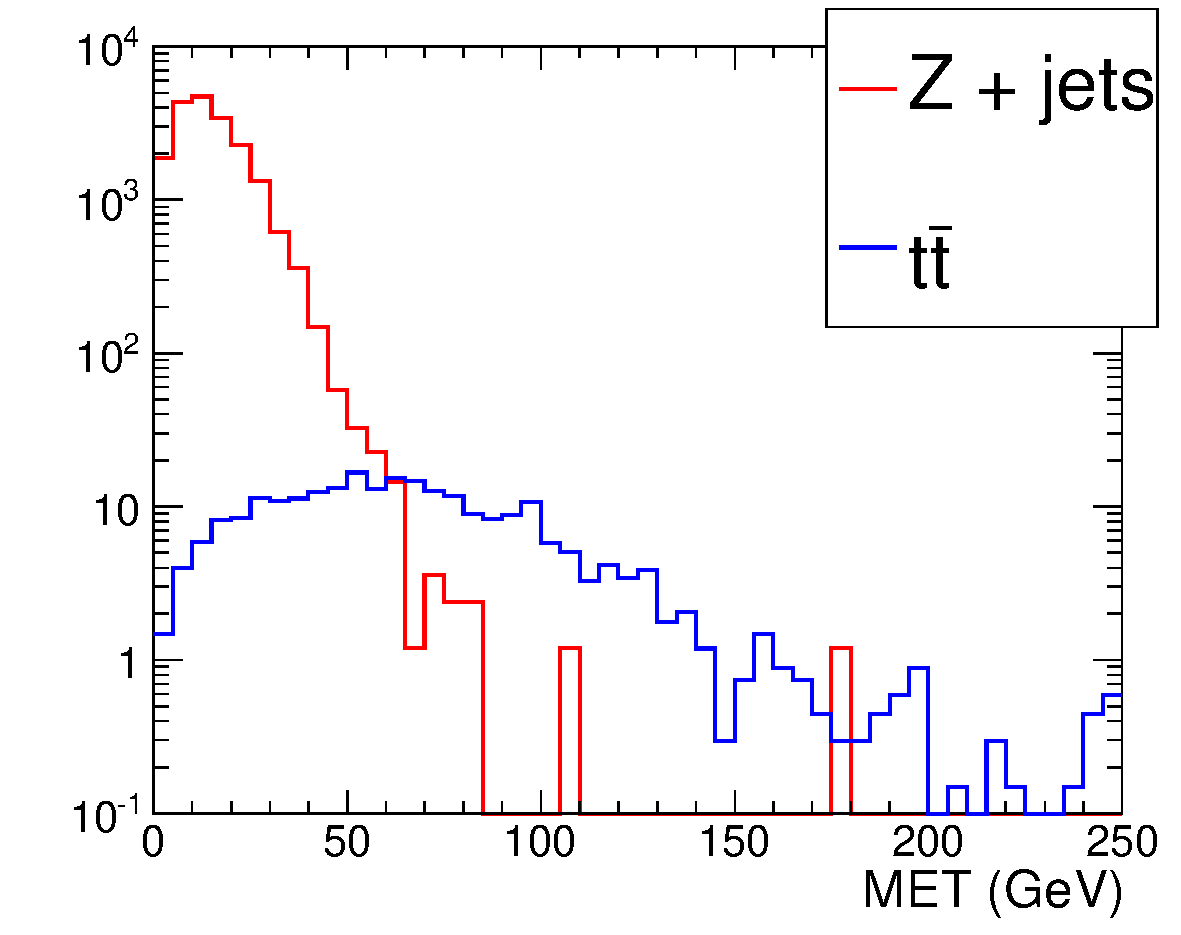
\includegraphics[width=0.75\linewidth]{plots/met_ttbar_Z.pdf}
\caption{\label{fig:metdist}\protect Distributions of MET in $Z$ and $t\bar{t}$ MC normalized to \lumi.}
\end{center}
\end{figure}

We define two signal regions for our search:
\begin{itemize}
\item MET $>$ 60 GeV (loose signal region):
In this region of MET there is a contribution from the tail of the MET distribution 
in \Z plus jets events. There is also a contribution from \ttbar events where the leptons happen to be in the \Z 
mass window. 
%We expect the MC simulation to do a good job on the second source, as it is well within the 
%bulk of the \ttbar phase space. However, for the first we must rely on data driven procedures. 

The MC and data yields for this signal region are given in Table~\ref{sigyieldtable60} and the dilepton
mass distributions are shown in Fig.~\ref{fig:dilmass60}.

More information on the data events in this signal region is given in Table~\ref{sig60events} and information 
on the muons in these events is given in Table~\ref{sig60muons}.

\item MET $>$ 120 GeV (tight signal region):
This signal region was selected by picking a region where the SM prediction 
for the dataset we have is  $\approx$ 1 event. 
At this kinematical region the dominant background contribution is expected to be from \ttbar.

The MC and data yields for this signal region are given in Table~\ref{sigyieldtable120}.
\end{itemize}

\noindent The data driven technique used to predict the missing transverse energy accompanying 
a \Z event is described in Section~\ref{sec:templates}.

\noindent To estimate the \ttbar background we will use the opposite flavor subtraction
 described in Section~\ref{sec:topbkg}.


\begin{figure}[hbt]
\begin{center}
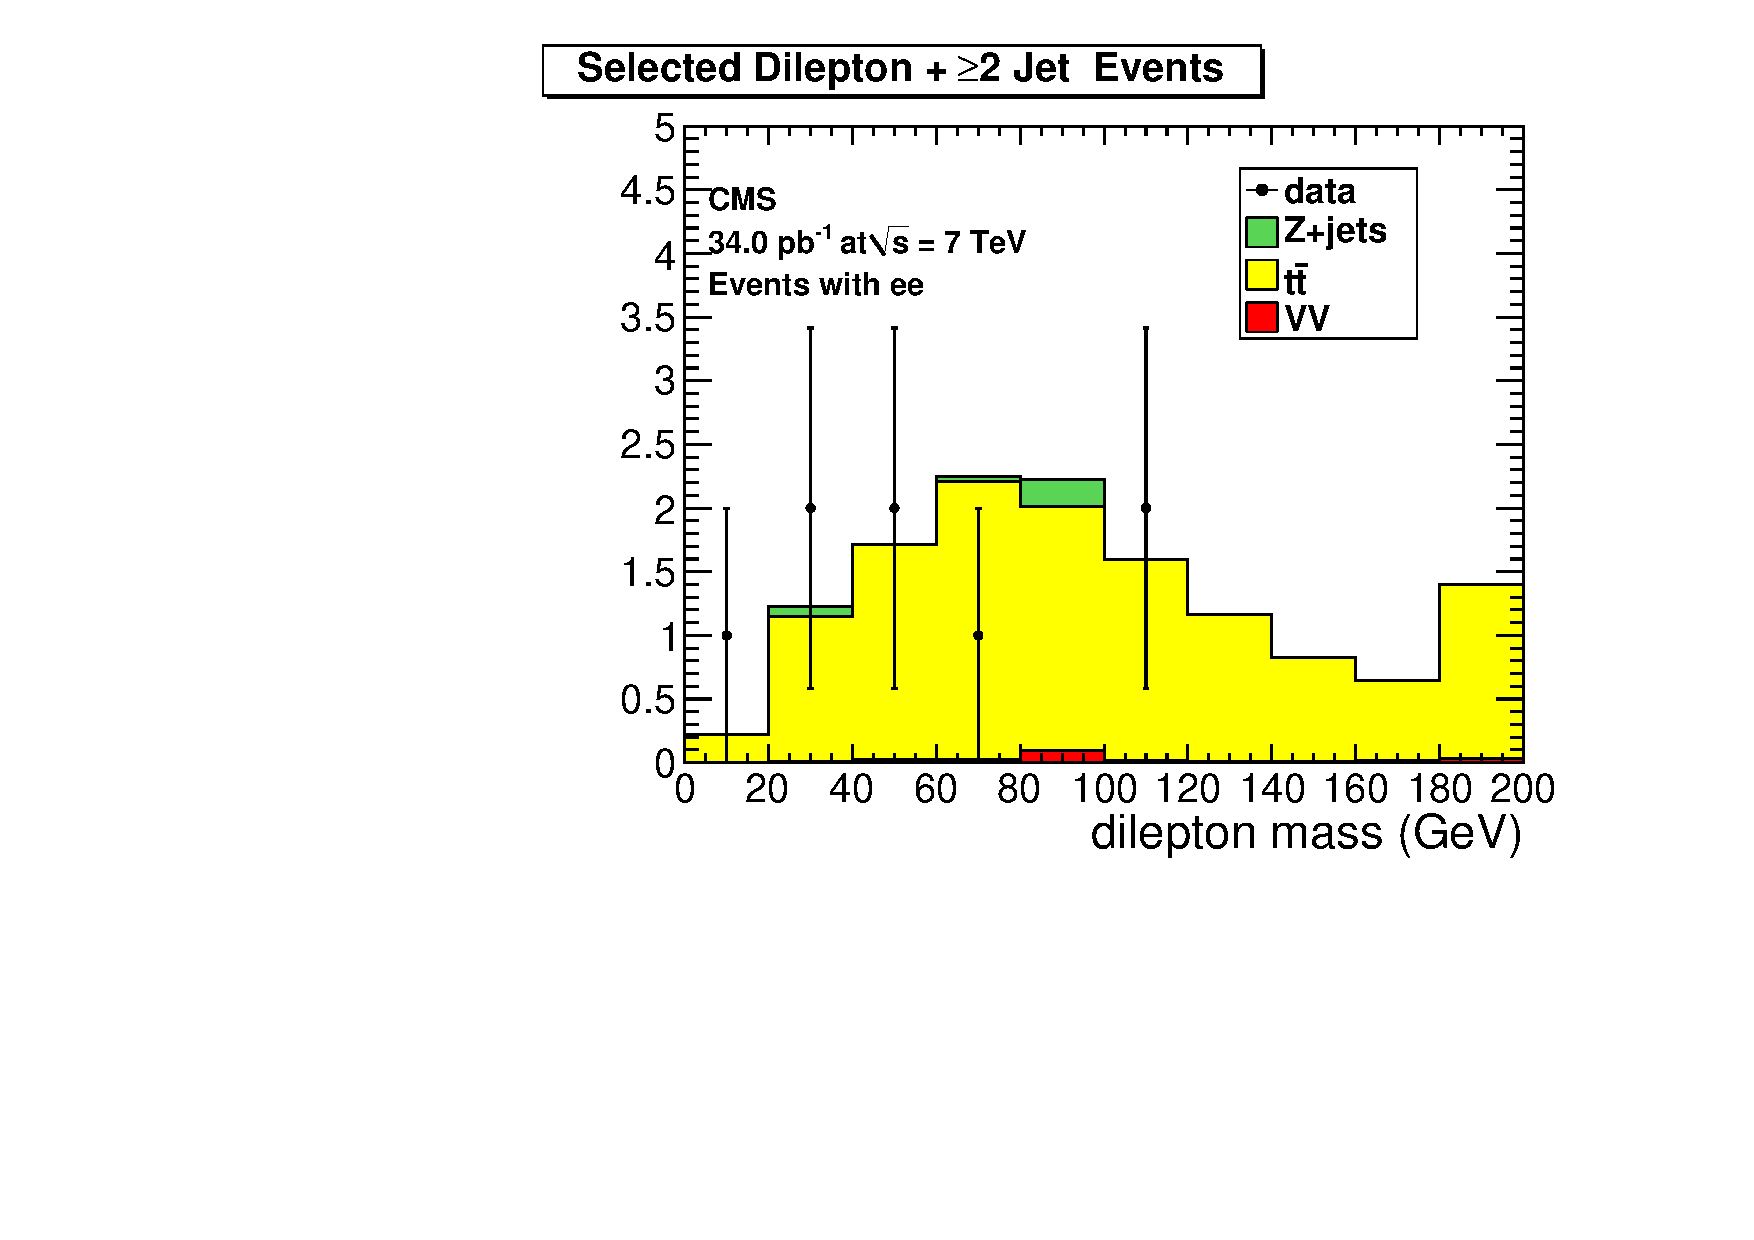
\includegraphics[width=0.48\linewidth]{plots/hdilmass_pfmet60_ee_allj.pdf}
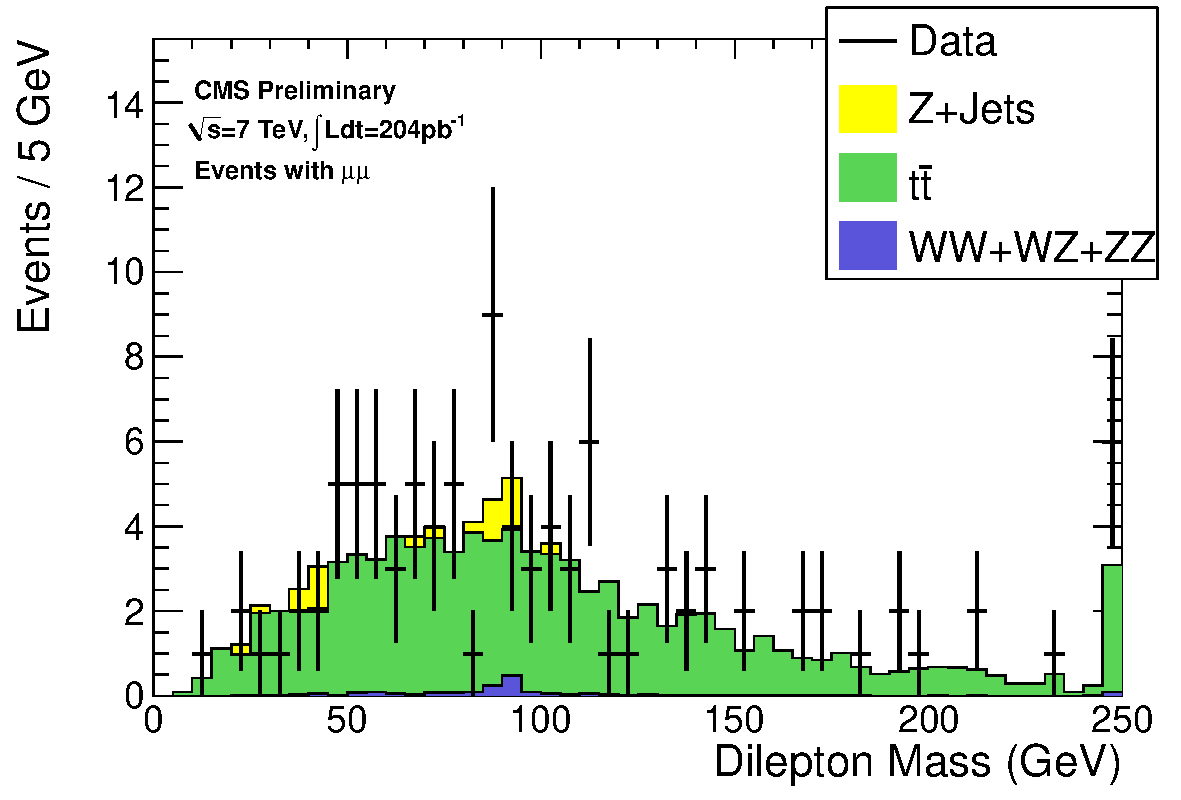
\includegraphics[width=0.48\linewidth]{plots/hdilmass_pfmet60_mm_allj.pdf}
\caption{\label{fig:dilmass60}\protect Dilepton mass distribution for events passing the pre-selection 
  and MET $>$ 60~GeV for \lumi\ in the $ee$ (left) and $\mu\mu$ (right) final states. Backgrounds from single top 
  and $W$+jets are omitted since they are negligible.}
\end{center}
\end{figure}

\begin{table}[htb]
\begin{center}
\caption{\label{sigyieldtable60} Data and Monte Carlo yields for the loose signal region MET $>$ 60~GeV  for \lumi.}
\begin{tabular}{lccccc}
%%%official PVT json v3, 38X MC 
\hline
              Sample   &                $ee$   &            $\mu\mu$   &              $e\mu$   &                 tot  \\
\hline
               ZJets   &     0.21 $\pm$ 0.09   &     0.21 $\pm$ 0.09   &     0.04 $\pm$ 0.04   &     0.46 $\pm$ 0.14  \\
               TTbar   &     1.89 $\pm$ 0.09   &     2.04 $\pm$ 0.09   &     4.17 $\pm$ 0.13   &     8.11 $\pm$ 0.18  \\
               WJets   &     0.00 $\pm$ 0.00   &     0.00 $\pm$ 0.00   &     0.00 $\pm$ 0.00   &     0.00 $\pm$ 0.00  \\
                  WW   &     0.01 $\pm$ 0.00   &     0.02 $\pm$ 0.00   &     0.03 $\pm$ 0.01   &     0.06 $\pm$ 0.01  \\
                  WZ   &     0.06 $\pm$ 0.00   &     0.06 $\pm$ 0.00   &     0.00 $\pm$ 0.00   &     0.12 $\pm$ 0.00  \\
                  ZZ   &     0.03 $\pm$ 0.00   &     0.03 $\pm$ 0.00   &     0.00 $\pm$ 0.00   &     0.06 $\pm$ 0.00  \\
                  tW   &     0.06 $\pm$ 0.01   &     0.06 $\pm$ 0.01   &     0.14 $\pm$ 0.01   &     0.26 $\pm$ 0.01  \\
\hline
           tot SM MC   &     2.26 $\pm$ 0.13   &     2.43 $\pm$ 0.13   &     4.39 $\pm$ 0.13   &     9.07 $\pm$ 0.22  \\
\hline
                data   &                   0   &                   7   &                   3   &                  10  \\
\hline
                 LM4   &     0.42 $\pm$ 0.01   &     0.44 $\pm$ 0.01   &     0.07 $\pm$ 0.01   &     0.93 $\pm$ 0.02  \\
                 LM8   &     0.19 $\pm$ 0.01   &     0.22 $\pm$ 0.01   &     0.07 $\pm$ 0.00   &     0.48 $\pm$ 0.01  \\
\hline
\end{tabular}
\end{center}
\end{table}



\begin{table}[htb]
\begin{center}
\caption{\label{sig60events} Details of data events for the loose signal region MET $>$ 60~GeV for \lumi. 
All 7 events are in the $\mu\mu$ final states. The SimpleSecondaryVertexTagger high efficiency medium 
working point is used for b-tagging, for which the efficiency is $\sim40$\% and the mistag rate is $\sim1$\%.}
\begin{tabular}{rrrrrrrrrr}

\hline

Run & Lumi & Event & Njet & N B Tag & pfMET & tcMET & Dilep Mass & Sum & Z \pt\\
 &  Section &  &  &  &  &  &  & jet \pt &  \\
\hline
147216 & 48 & 35885648 & 2 & 0 & 78.9 & 72.9 & 95.0 & 216.4 & 116.4\\
147217 & 75 & 55188718 & 2 & 0 & 79.7 & 67.8 & 90.7 & 75.7 & 39.1\\
147450 & 82 & 29253181 & 5 & 0 & 63.6 & 70.8 & 97.9 & 429.5 & 312.0\\
148862 & 350 & 522383338 & 4 & 1 & 90.0 & 75.7 & 82.4 & 373.4 & 87.0\\
149181 & 1769 & 1675896175 & 2 & 1 & 67.8 & 64.4 & 97.2 & 163.9 & 128.6\\
149291 & 205 & 199787369 & 4 & 0 & 74.5 & 92.9 & 85.0 & 303.1 & 64.3\\
149291 & 232 & 235101408 & 2 & 1 & 87.3 & 90.0 & 88.7 & 315.4 & 32.4\\

\hline
\end{tabular}
\end{center}
\end{table}


\begin{table}[htb]
\begin{center}
\caption{\label{sig60muons} Details of the muons in events in the loose signal region MET $>$ 60~GeV for \lumi. 
Shown are the transverse momentum, the relative error in the transverse momentum, d0 calculated with respect to the beamspot,
the number of hits in the Silicon track, the number of layers crossed by the Silicon track, the normalized $\chi^2$,
whether a muon segment was found in the last chamber traversed by the muon, and the number of hits in the muon chambers used in the global fit. }
\begin{tabular}{rrrrrrrrrr}
\hline

Event & Si \pt &  Si \pt & gfit \pt & d0 & N Si Hits & N Si & Si $\chi^2$ & TMLast & gfit STA \\
 &  &  rel err &  &  &  &  Layers &  & Station & hits \\
 &  &  &  &  &  &  &  & Loose &  \\
\hline
35885648 & 110.2 & 0.030 & 111.3 & -0.001 & 29 & 15 & 0.65 & 1 & 18 \\
35885648 & 27.5 & 0.012 & 27.5 & 0.005 & 16 & 12 & 0.26 & 1 & 18 \\
55188718 & 22.4 & 0.017 & 22.4 & -0.003 & 15 & 10 & 0.93 & 1 & 25 \\
55188718 & 46.7 & 0.016 & 46.9 & 0.007 & 19 & 13 & 0.79 & 1 & 35 \\
29253181 & 71.2 & 0.026 & 70.5 & -0.011 & 25 & 15 & 0.78 & 1 & 13 \\
29253181 & 255.7 & 0.068 & 301.0 & -0.011 & 24 & 15 & 0.69 & 1 & 13 \\
522383338 & 89.1 & 0.018 & 89.4 & -0.000 & 16 & 12 & 0.43 & 1 & 26 \\
522383338 & 27.1 & 0.011 & 27.1 & -0.004 & 16 & 12 & 0.13 & 1 & 36 \\
1675896175 & 80.3 & 0.017 & 80.1 & 0.002 & 19 & 13 & 0.60 & 1 & 32 \\
1675896175 & 77.6 & 0.016 & 77.5 & -0.000 & 17 & 13 & 0.21 & 1 & 25 \\
199787369 & 22.6 & 0.018 & 22.5 & -0.000 & 21 & 14 & 0.59 & 1 & 12 \\
199787369 & 82.0 & 0.033 & 80.9 & -0.002 & 12 & 10 & 0.61 & 1 & 14 \\
235101408 & 30.6 & 0.014 & 30.9 & -0.007 & 16 & 11 & 0.14 & 1 & 29 \\
235101408 & 59.7 & 0.013 & 59.9 & 0.006 & 20 & 13 & 0.37 & 1 & 16 \\


\hline
\end{tabular}
\end{center}
\end{table}



\begin{table}[htb]
\begin{center}
\caption{\label{sigyieldtable120} Data and Monte Carlo yields for the loose signal region MET $>$ 120~GeV  for \lumi.}
\begin{tabular}{lccccc}
%%%official PVT json v3, 38X MC
\hline
              Sample   &                $ee$   &            $\mu\mu$   &              $e\mu$   &                 tot  \\
\hline
               ZJets   &     0.00 $\pm$ 0.00   &     0.00 $\pm$ 0.00   &     0.00 $\pm$ 0.00   &     0.00 $\pm$ 0.00  \\
               TTbar   &     0.26 $\pm$ 0.03   &     0.28 $\pm$ 0.03   &     0.55 $\pm$ 0.05   &     1.09 $\pm$ 0.06  \\
               WJets   &     0.00 $\pm$ 0.00   &     0.00 $\pm$ 0.00   &     0.00 $\pm$ 0.00   &     0.00 $\pm$ 0.00  \\
                  WW   &     0.00 $\pm$ 0.00   &     0.00 $\pm$ 0.00   &     0.00 $\pm$ 0.00   &     0.01 $\pm$ 0.00  \\
                  WZ   &     0.01 $\pm$ 0.00   &     0.01 $\pm$ 0.00   &     0.00 $\pm$ 0.00   &     0.02 $\pm$ 0.00  \\
                  ZZ   &     0.01 $\pm$ 0.00   &     0.01 $\pm$ 0.00   &     0.00 $\pm$ 0.00   &     0.02 $\pm$ 0.00  \\
                  tW   &     0.00 $\pm$ 0.00   &     0.01 $\pm$ 0.00   &     0.02 $\pm$ 0.00   &     0.03 $\pm$ 0.00  \\
\hline
           tot SM MC   &     0.29 $\pm$ 0.03   &     0.31 $\pm$ 0.03   &     0.58 $\pm$ 0.05   &     1.17 $\pm$ 0.07  \\
\hline
                data   &                   0   &                   0   &                   0   &                   0  \\
\hline
                 LM4   &     0.33 $\pm$ 0.01   &     0.35 $\pm$ 0.01   &     0.06 $\pm$ 0.01   &     0.74 $\pm$ 0.02  \\
                 LM8   &     0.14 $\pm$ 0.01   &     0.16 $\pm$ 0.01   &     0.06 $\pm$ 0.00   &     0.36 $\pm$ 0.01  \\
\hline
\end{tabular}
\end{center}
\end{table}


\clearpage

\section{MET Templates}
\label{sec:templates}

The background from SM $Z$ production accompanied by artificial MET from detector mismeasurements
is estimated using the novel MET templates technique.
The premise of this data driven technique is that MET in \Z plus jets events
is produced by the hadronic recoil system and {\it not} by the leptons making up the \Z.
Therefore, the MET distribution in these events can be modeled using a control sample
which has no true MET and the same general attributes regarding fake MET as in \Z plus jets events.
We use two complementary control samples: one consisting of photon plus jets events, and one
consisting of QCD multijet events. 

Photon plus jets events are selected from a set of single photon
triggers with varying photon \pt\ thresholds, and QCD multijet events are selected from a set
of single jet triggers with varying jet \pt\ thresholds. 
In the \Z plus jets events as well as in both control samples, the MET is dominated by mismeasurements
of the hadronic system. To account for kinematic 
differences between the hadronic systems in the control vs. signal samples, 
we measure the MET distributions in the control samples in bins of the number of jets and the 
scalar sum of the transverse energies of the jets (\Ht), separately for each of the single photon and single jet trigger thresholds.
Each MET distribution is normalized to unit area, yielding an
array of MET templates. Each \Z event is then assigned one such unit area template based on its number of jets and \Ht.
The trigger threshold is chosen based on the \Z \pt\ (leading jet \pt) for the photon plus
jets (QCD multijets) control sample.
The sum of the templates for all selected \Z events then forms the 
prediction of the MET distribution for the \Z sample. Integrating this prediction for our 
signal regions  thus provides a data driven prediction for the \Z plus jets yields in the 
signal regions. 

We use 2 separate control samples, since each has relative advantages. The photon plus jets events have a topology
which is more similar to the \Z plus jets events, since both consist of a well-measured
object recoiling against a system of hadronic jets. Possible contributions of the photon
to the MET in the event are eliminated in the QCD multijet sample. We have verified that
the predictions from the 2 control samples are consistent within their uncertainties, and
choose to use the prediction from the photon plus jets sample.
By using two independent control samples, we are able to illustrate
the robustness of the MET templates method and to cross check the data driven background 
prediction.

The systematic uncertainty in the prediction from the photon plus jets MET templates
originates from 2 sources. Possible contributions to the MET from the photon are assessed
by varying the photon selection, which leads to a relative difference in the predicted
background of 15\%. The effect of the difference between the distributions of hadronic recoil \pt\
in the control vs. signal samples is estimated by reweighting the photon plus jets events such
that the hadronic recoil \pt distribution matches that in \Z plus jets events, leading to a relative
difference in the predicted background of 20\%. The total uncertainty in the predicted background
from the MET templates method is 25\%.


\section{Closure Test of Templates in MC}
\label{sec:mc}

The above procedure is applied to MC to test its effectiveness under `ideal' conditions. 
In order to test the 
results obtained in section \ref{sec:tempcompresults}, 
%dependence of the method on the sample composition, 
we construct templates separately from PhotonJet MC and QCD MC.
%Templates are derived from PhotonJet MC, and 
These templates are then used to predict the MET distribution in ZJets MC. The 
MC samples used are:

\begin{itemize}
\item PhotonJet MC
  \begin{itemize}
  \item \verb=/G_Pt_15to30_TuneZ2_7TeV_pythia6/Spring11-PU_S1_START311_V1G1-v1/AODSIM  =
  \item \verb=/G_Pt_30to50_TuneZ2_7TeV_pythia6/Spring11-PU_S1_START311_V1G1-v1/AODSIM  =
  \item \verb=/G_Pt_50to80_TuneZ2_7TeV_pythia6/Spring11-PU_S1_START311_V1G1-v1/AODSIM  =
  \item \verb=/G_Pt_80to120_TuneZ2_7TeV_pythia6/Spring11-PU_S1_START311_V1G1-v1/AODSIM =
  \item \verb=/G_Pt_120to170_TuneZ2_7TeV_pythia6/Spring11-PU_S1_START311_V1G1-v1/AODSIM=
  \item \verb=/G_Pt_170to300_TuneZ2_7TeV_pythia6/Spring11-PU_S1_START311_V1G1-v1/AODSIM= 	  
  \end{itemize}
\item QCD MC
  \begin{itemize}
  \item \verb=/QCD_Pt_15to30_TuneZ2_7TeV_pythia6/Spring11-PU_S1_START311_V1G1-v1/AODSIM  =
  \item \verb=/QCD_Pt_30to50_TuneZ2_7TeV_pythia6/Spring11-PU_S1_START311_V1G1-v1/AODSIM  =
  \item \verb=/QCD_Pt_50to80_TuneZ2_7TeV_pythia6/Spring11-PU_S1_START311_V1G1-v1/AODSIM  =
  \item \verb=/QCD_Pt_80to120_TuneZ2_7TeV_pythia6/Spring11-PU_S1_START311_V1G1-v1/AODSIM =
  \item \verb=/QCD_Pt_120to170_TuneZ2_7TeV_pythia6/Spring11-PU_S1_START311_V1G1-v1/AODSIM= 
  \item \verb=/QCD_Pt_170to300_TuneZ2_7TeV_pythia6/Spring11-PU_S1_START311_V1G1-v1/AODSIM= 
  \end{itemize}
\item ZJet MC
  \begin{itemize}
  \item \verb=/DYToEE_M-20_CT10_TuneZ2_7TeV-powheg-pythia/Spring11-PU_S1_START311_V1G1-v1/AODSIM=
  \item \verb=/DYToMuMu_M-20_CT10_TuneZ2_7TeV-powheg-pythia/Spring11-PU_S1_START311_V1G1-v1/AODSIM=
  \item \verb=/DYToTauTau_M-20_CT10_TuneZ2_7TeV-powheg-pythia-tauola/Spring11-PU_S1_START311_V1G1-v1/AODSIM=
	%use pythia
	%\item \verb=/DYJetsToLL_TuneD6T_M-50_7TeV-madgraph-tauola/Spring11-PU_S1_START311_V1G1-v1/AODSIM=
  \end{itemize}
\end{itemize}


Good agreement between the observed and predicted MET distributions is observed for each MC sample, as well as between the two samples, as shown in figures \ref{fig:mcclosurepho} and \ref{fig:mcclosureqcd}.

\begin{figure}[hbt]
  \begin{center}
    \resizebox{0.8\linewidth}{!}{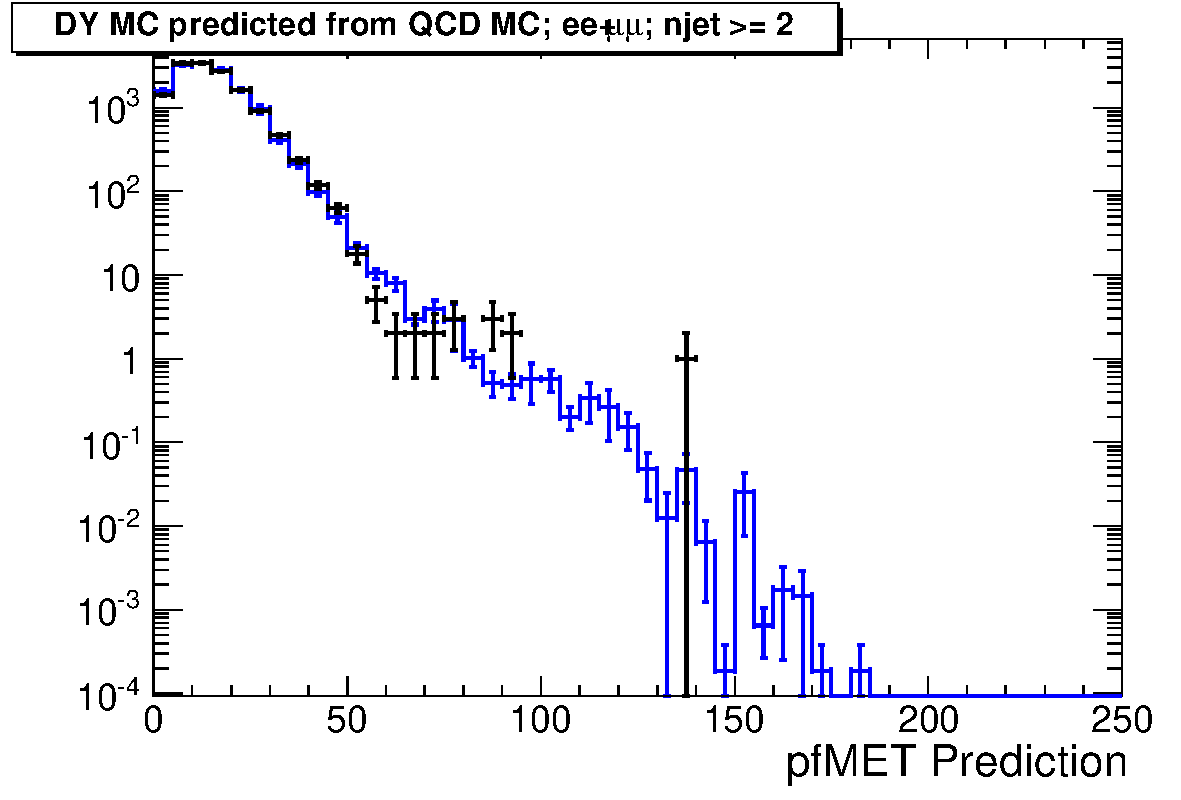
\includegraphics{plots/mcclosure_qcd.pdf}}
	\\ \medskip
    %\resizebox{\linewidth}{!}{
    \begin{tabular}{r|r|r|r|r}
      MET        & $>$ 30 GeV       & $>$ 60 GeV        & $>$ 100 GeV       & $>$ 200  \\ \hline

%tr
	  Z MC       &   921               &    15               &     1               &     0 \\
	  Prediction & 824.20 $\pm$  38.99 &  21.89 $\pm$   2.52 &   1.67 $\pm$   0.31 &   0.00 $\pm$   0.00 \\

%no tr
	  %  data    &   921               &    15               &     1               &     0 \\
	  %  pred    & 751.10 $\pm$ 101.82 &   7.78 $\pm$   0.53 &   0.45 $\pm$   0.06 &   0.00 $\pm$   0.00 \\

    \end{tabular}
	%}
	\\ \medskip
    \caption{The MET distribution in \Z plus jets MC (black) and prediction (blue) for Njet $\ge$ 2. 
	  Below the plot is tabulated the integral of the \Z plus jets MC MET and the predicted 
	  MET from QCD MC for 
	  MET $>$ 30 GeV, $>$ 60 GeV, $>$ 100 GeV, and $>$ 200 GeV. 
	}
    \label{fig:mcclosureqcd}
  \end{center}
\end{figure}


\begin{figure}[hbt]
  \begin{center}
    \resizebox{0.8\linewidth}{!}{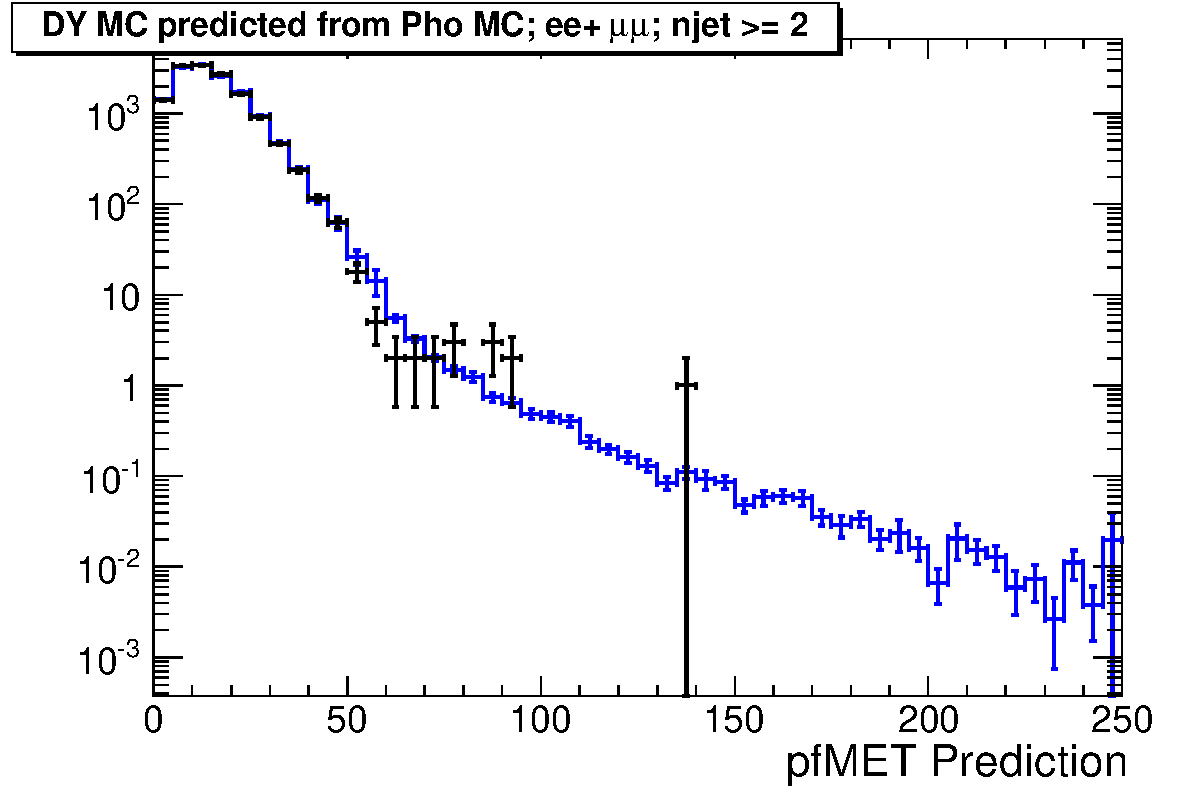
\includegraphics{plots/mcclosure_pho.pdf}}
	\\ \medskip
    %\resizebox{\linewidth}{!}{
    \begin{tabular}{r|r|r|r|r}
      MET        & $>$ 30 GeV       & $>$ 60 GeV        & $>$ 100 GeV       & $>$ 200  \\ \hline
%tr
	  Z MC       &   921               &    15               &     1               &     0 \\
	  Prediction & 959.15 $\pm$  27.00 &  19.39 $\pm$   0.58 &   2.28 $\pm$   0.09 &   0.07 $\pm$   0.01 \\
	  
%no tr
%	  Z MC       &   921               &    15               &     1               &     0 \\
%	  Prediction & 953.60 $\pm$  31.28 &  17.94 $\pm$   0.66 &   2.45 $\pm$   0.10 &   0.11 $\pm$   0.02 \\

    \end{tabular}
	%}
	\\ \medskip
    \caption{The MET distribution in \Z plus jets MC (black) and prediction (blue) for Njet $\ge$ 2. 
	  Below the plot is tabulated the integral of the \Z plus jets MC MET and the predicted 
	  MET from photon plus jets MC for 
	  MET $>$ 30 GeV, $>$ 60 GeV, $>$ 100 GeV, and $>$ 200 GeV. 
	}
    \label{fig:mcclosurepho}
  \end{center}
\end{figure}


%2010 results
%      MET                   & $>$ 30 GeV & $>$ 60 GeV  & $>$ 120 GeV \\ \hline
%      Z+jets observed         &      184   &    10       & 0          \\
%      $\gamma$+jets predicted &   182.21   &    11.52    & 1.40       \\


%\begin{wrapfigure}{r}{0.6\textwidth}
%\vspace{-25pt}
%\begin{center}
%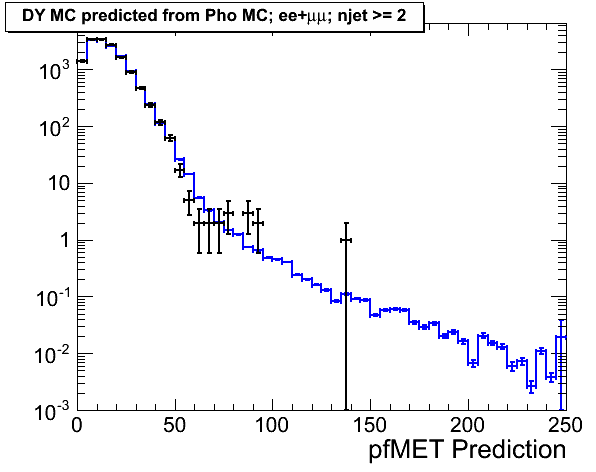
\includegraphics[width=0.8\textwidth]{plots/mcclosure}
% \caption{\label{fig:mcclosure} The MET distribution in Z+jets MC (black) and prediction (blue) for Njet $\ge$ 2. Below the plot is tabulated the integral of the observed Z+jets MC MET and the predicted MET from $\gamma$+jets MC for MET $>$ 30 GeV, $>$ 60 GeV and $>$ 120 GeV. The quantity (observed-predicted)/predicted as a function of MET is shown above the plot.}
%\end{center}
%\vspace{-20pt}
%\end{wrapfigure}

\clearpage

\section{Top Background Estimation}
\label{sec:topbkg}

The \ttbar\ contribution to the signal region is estimated using an opposite-flavor (OF) subtraction technique.
This technique takes advantage of the fact that the \ttbar\ yield in the 
OF final state ($e\mu$) is the same as in the same-flavor (SF) final state
($ee+\mu\mu$), modulo differences in efficiency in the $e$ vs. $\mu$ selection.
Hence the \ttbar\ yield in the same-flavor final state can be estimated
using the corresponding yield in the opposite-flavor final state. 
Other backgrounds for which the lepton flavors are
uncorrelated (for example, $W^+W^-$ and DY$\rightarrow \tau^+\tau^-$) are also included in
this estimate.

To predict the SF yield in a signal region defined by a requirement on the MET, we take the 
OF yield passing the same MET requirement. This yield is corrected using the ratio of
muon to electron selection efficiencies $R_{\mu e}=1.07 \pm 0.03$.
This quantity is evaluated from studies of $Z\to\mu^+\mu^-$ and $Z\to e^+e^-$
events in data. To improve the statistical precision
of the background estimate, we do not require the OF events to lie in the $Z$ mass region,
and we apply a scale factor $K=0.16 \pm 0.01$ accounting for the fraction of \ttbar\ events
which lie in the region $81 < \mathrm{M(\ell\ell)} < 101$\GeVcc, extracted from MC.

Backgrounds from pair production of vector bosons are negligible compared to $t\bar{t}$.
Backgrounds from fake leptons are negligible due to the requirement of two \pt$ > 20$~GeV leptons
in the \Z mass window, accompanied by jets and large MET.

%\subsection{Non $t\bar{t}$ Backgrounds}
%\label{sec:othBG}

Backgrounds  in  which one  or  both  leptons  do not  originate  from
electroweak decays  (non-$W/Z$ leptons) are assessed  using the method
of  Ref.~\cite{ref:top}.  A non-$W/Z$  lepton is  a lepton  candidate
originating from within a jet,  such as a lepton from semileptonic $b$
or  $c$ decays,  a muon  decay-in-flight, a  pion misidentified  as an
electron,  or an  unidentified  photon conversion.   Estimates of  the
contributions to  the signal region  from pure multijet QCD,  with two
non-$W/Z$ leptons, and in $W+\mathrm{jets}$, with one non-$W/Z$ lepton
in  addition to  the lepton  from the  decay of  the $W$,  are derived
separately. We find $0.00^{+0.04}_{-0.00}$ and $0.0^{+0.5}_{-0.0}$ 
($0.00^{+0.04}_{-0.00}$ and $0.5 \pm 0.5$)
for the  multijet QCD  and $W$+jets  contributions to the high \MET\
(high \Ht) signal regions, respectively,  and thus
consider these backgrounds to be negligible.

Backgrounds from DY are estimated with the data-driven $R_{out/in}$ technique~\cite{ref:top},
which leads to an estimated DY contribution which is consistent with 0.
Backgrounds from processes with two vector bosons and single top 
are negligible compared to dilepton $t\bar{t}$. 

\section{Results}
\label{sec:results}

\subsection{Background estimate from the ABCD method}
\label{sec:abcdres}

We begin by applying the ABCD method to estimate the background in the 2010 signal region.
The data yields in the four regions are summarized in Tables~\ref{tab:datayield1} and
the $y$ vs. \Ht\ distributions are displayed in Fig.~\ref{fig:abcdData1}.
The ABCD background prediction is $N_A \times N_C / N_B = 12.7 \pm 2.4$ (stat), in
agreement with the MC expectation. We also apply the ABCD' method to estimate the
background in this region, following the procedure of App.~\ref{app:abcdprime},
and find a predicted background of $12.8 \pm 2.9$ (stat), in good agreement
with the ABCD prediction.

Next, we apply the ABCD' method to predict the yields in the high \met\ and high \Ht\
signal regions. The $y$ vs. \Ht\ distributions for data are displayed in 
Fig.~\ref{fig:abcdprimedata}. The signal regions are indicated, as well as the control 
regions used to measure the $f(y)$ and $g(H_T)$ distributions. For the high \met\
signal region, we find a predicted yield of $1.0 \pm 0.3$ (stat), in reasonable
agreement with the MC prediction. For the high \Ht\ signal region, we do not find
any events in the control region used to extract $g(H_T)$ with \Ht\ $>$ 600 GeV,
and the ABCD' background estimate is therefore 0. To assess the statistical uncertainty
in this prediction, we add a single event ``by hand'' to the $g(H_T)$ distributiion
at $H_T = 600$ GeV, leading to a predicted yield of 0.6. 
{\bf NEED TO THINK ABOUT THIS. THE PREDICTION DEPENDS ON WHERE IN HT YOU PUT THIS }
{\bf SINGLE EVENT. FOR EXAMPLE, PUTTING IT AT 1000 GIVES A PREDICTION OF 1.2      }
{\bf HOPEFULLY WITH ~3X MORE STATS WE WON'T BE IN THIS SITUATION                  }
These results are summarized in Table~\ref{tab:abcdprime}.

\begin{table}[hbt]
\begin{center}
\caption{\label{tab:abcdprime} 
Summary of results of the ABCD' method, applied to the 3 signal regions. The correction
factors are given in Table~\ref{tab:cor}.
}
\begin{tabular}{lccccc}
\hline
Signal Region             &     ABCD' pred      &  correction factor  &  prediction                                  \\ 
\hline
2010 signal region        &  $12.8 \pm 2.9$     & $1.0 \pm 0.2$      & 12.8 $\pm$ 2.9 (stat) $\pm$ 2.6 (syst)        \\
high \met\ signal region  &  $1.0  \pm 0.3$     & $1.2 \pm 0.5$      &  1.2 $\pm$ 0.4 (stat) $\pm$ 0.5 (syst)        \\
high \Ht\ signal region   &  $0.0  \pm 0.6$     & $1.0 \pm 0.5$      &  0.0 $\pm$ 0.6 (stat) $\pm$ 0.3 (syst)        \\
\hline
\end{tabular}
\end{center}
\end{table}

\begin{figure}[tbh]
\begin{center}
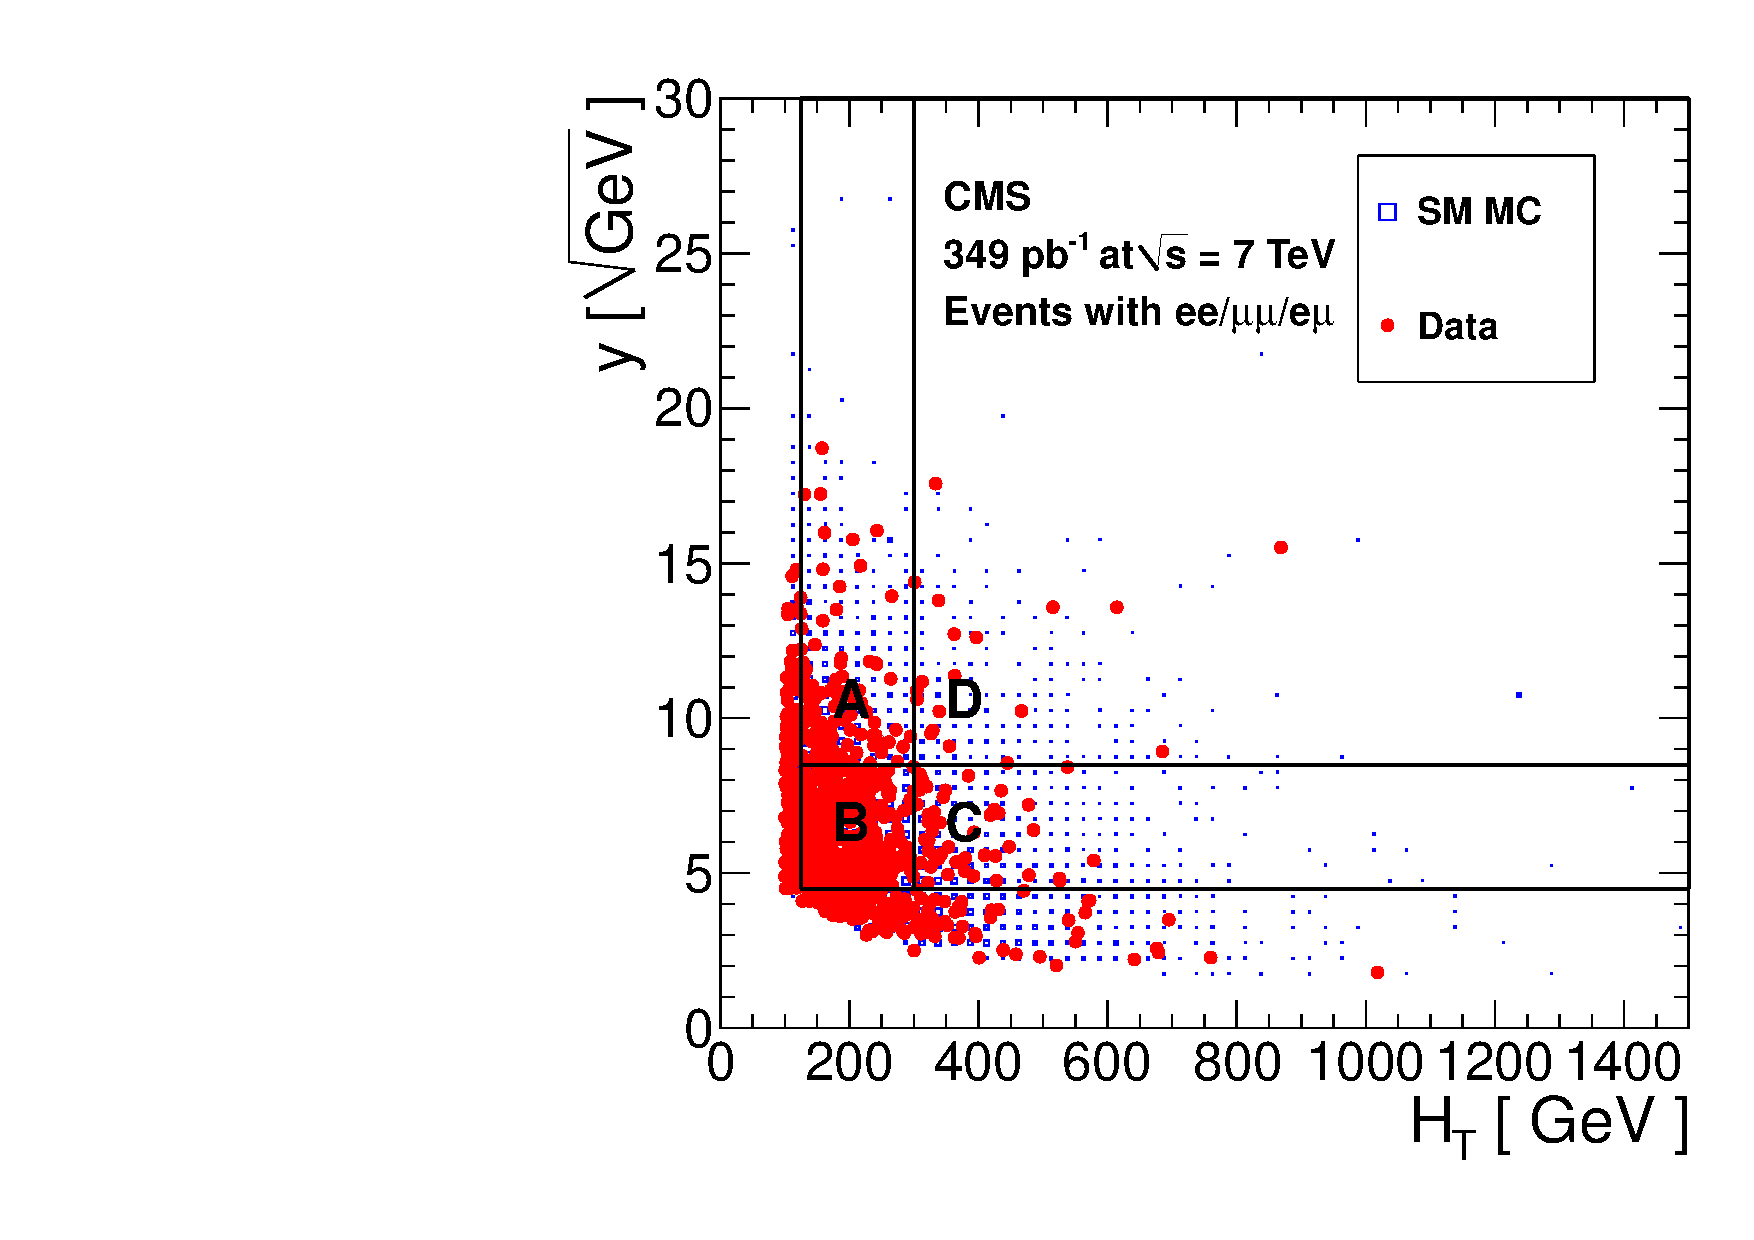
\includegraphics[width=0.6\linewidth]{plots/abcd_349pb.pdf}
\caption{\label{fig:abcdData1}\protect Distributions of $y$ 
vs. \Ht\ for SM Monte Carlo and data. The 2010 signal region boundaries are overlayed.}
\end{center}
\end{figure}

\begin{table}[hbt]
\begin{center}
\caption{\label{tab:datayield1} 
Data yields in the four
regions of Figure~\ref{fig:abcdData1} for the 2010 signal region, 
as well as the predicted yield in region D given
by $N_A \times N_C / N_B$.  The quoted uncertainty
on the prediction in data is statistical only, assuming Gaussian errors.
We also show the SM Monte Carlo expectations with statistical errors only.
}
\begin{tabular}{l||c|c|c|c||c}
\hline
           sample  &            $N_A$  &            $N_B$  &            $N_C$  &             $N_D$  &   $N_A \times N_C / N_B$ \\
\hline
            \ttll  & 63.9  $\pm$  2.0  &252.3  $\pm$  4.1  & 43.3  $\pm$  1.7  &  8.5  $\pm$  0.7  & 11.0  $\pm$  0.6        \\
           \tttau  & 18.5  $\pm$  1.1  & 55.9  $\pm$  1.9  & 10.3  $\pm$  0.8  &  3.4  $\pm$  0.5  &  3.4  $\pm$  0.4        \\
          \ttfake  &  1.0  $\pm$  0.3  &  6.6  $\pm$  0.7  &  1.1  $\pm$  0.3  &  0.4  $\pm$  0.2  &  0.2  $\pm$  0.1        \\
               DY  &  0.9  $\pm$  0.6  & 13.9  $\pm$  2.6  &  1.3  $\pm$  0.8  &  1.7  $\pm$  1.0  &  0.1  $\pm$  0.1        \\
              \WW  &  1.1  $\pm$  0.1  &  2.7  $\pm$  0.2  &  0.2  $\pm$  0.1  &  0.3  $\pm$  0.1  &  0.1  $\pm$  0.0        \\
              \WZ  &  0.1  $\pm$  0.0  &  0.6  $\pm$  0.0  &  0.1  $\pm$  0.0  &  0.0  $\pm$  0.0  &  0.0  $\pm$  0.0        \\
              \ZZ  &  0.0  $\pm$  0.0  &  0.2  $\pm$  0.0  &  0.0  $\pm$  0.0  &  0.0  $\pm$  0.0  &  0.0  $\pm$  0.0        \\
       single top  &  3.3  $\pm$  0.2  &  9.6  $\pm$  0.3  &  0.4  $\pm$  0.1  &  0.1  $\pm$  0.0  &  0.1  $\pm$  0.0        \\
           \wjets  &  1.0  $\pm$  1.0  &  2.2  $\pm$  1.1  &  0.0  $\pm$  0.0  &  0.0  $\pm$  0.0  &  0.0  $\pm$  0.0        \\
\hline
      Total SM MC  & 89.9  $\pm$  2.6  &344.0  $\pm$  5.3  & 56.6  $\pm$  2.1  & 14.5  $\pm$  1.4  & 14.8  $\pm$  0.7        \\
\hline
             data  &              110  &              381  &               44  &               19  & 12.7  $\pm$  2.4        \\
\hline
\end{tabular}
\end{center}
\end{table}


\begin{figure}[hbt]
\begin{center}
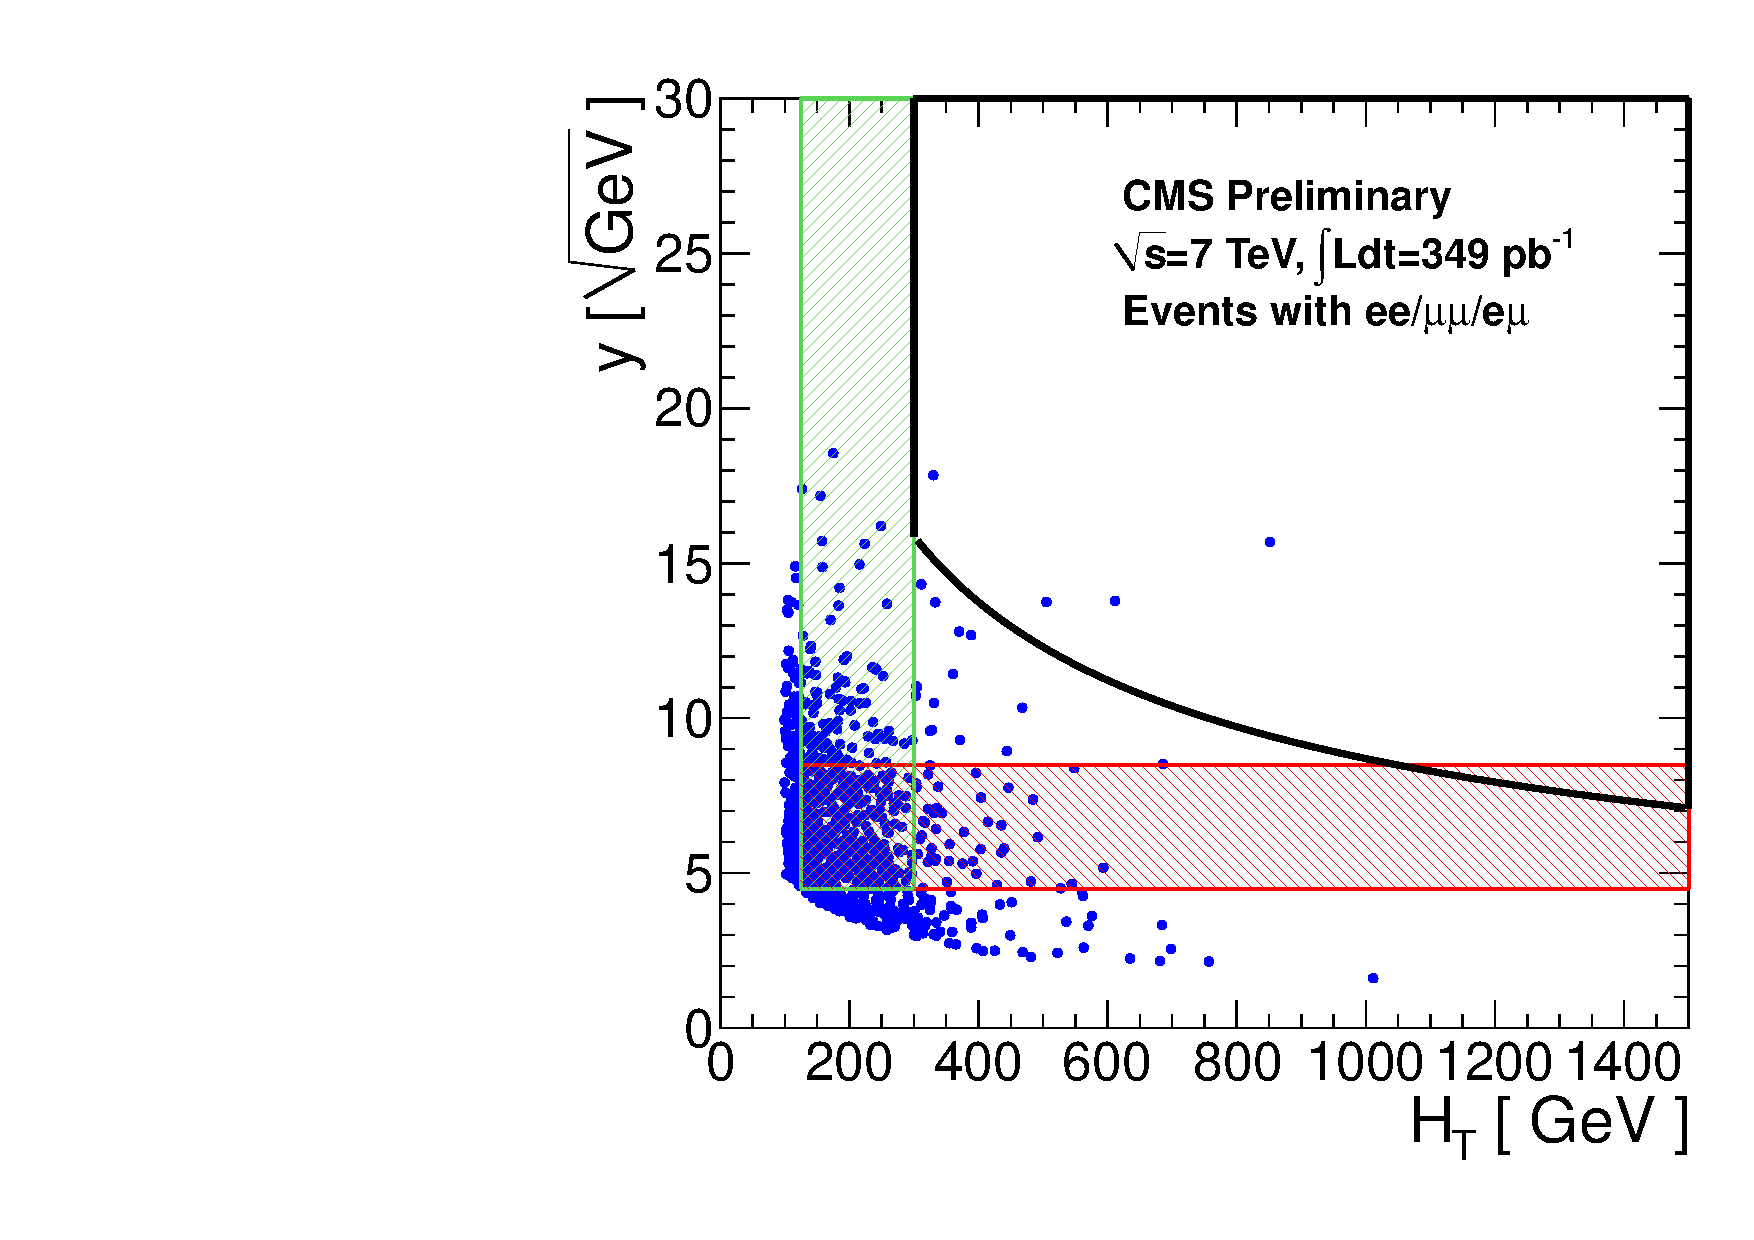
\includegraphics[width=0.48\linewidth]{plots/abcdprime_349pb_highmet.pdf}
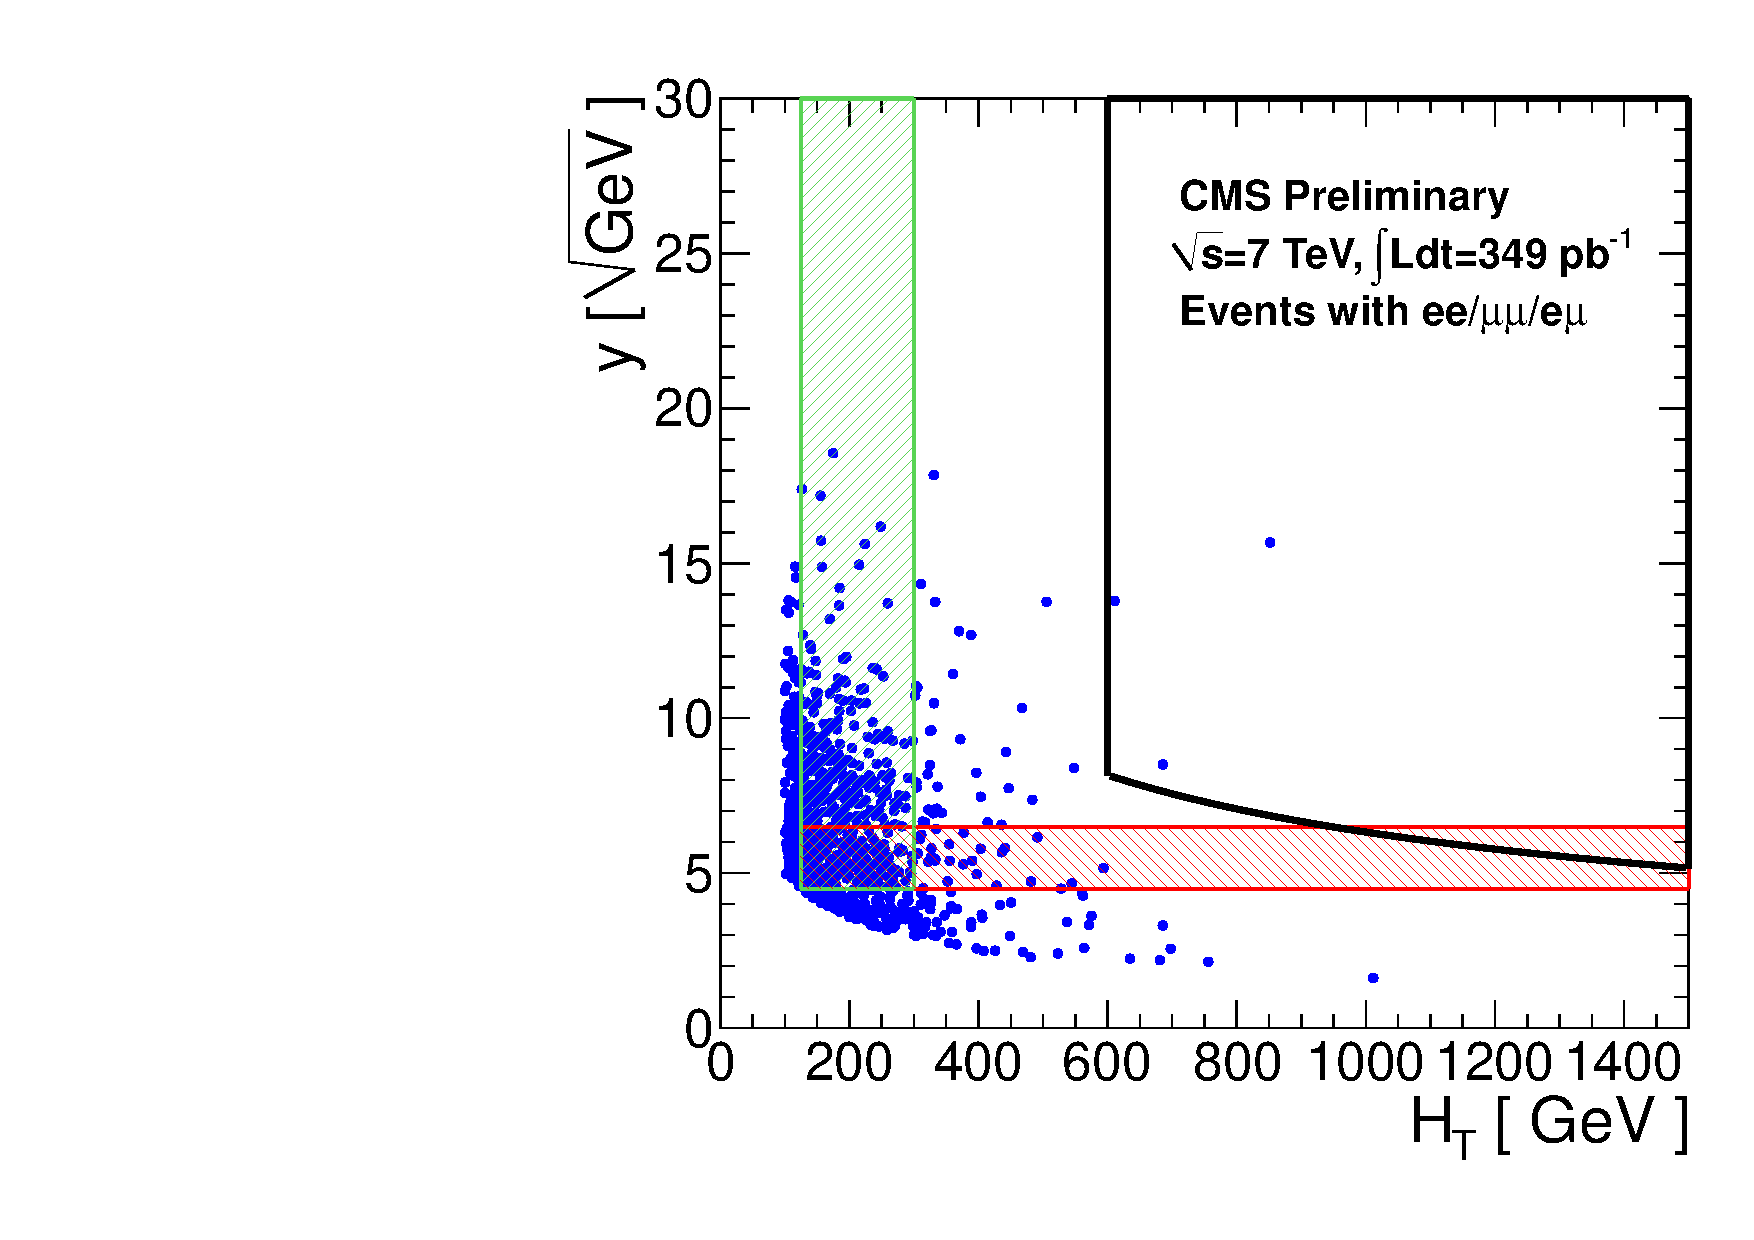
\includegraphics[width=0.48\linewidth]{plots/abcdprime_349pb_highht.pdf}
\caption{\label{fig:abcdprimedata}\protect 
Distributions of $y$ vs. \Ht\ in data. The signal regions \met\ $>$ 275 GeV, \Ht\ $>$ 300 GeV (left)
and \met\ $>$ 200 GeV, \Ht\ $>$ 600 GeV (right) are indicated with thick black lines. 
The $f(y)$ and $g(H_T)$ 
functions are measured using events in the green and red shaded areas, respectively.
}
\end{center}
\end{figure}

\subsection{Background estimate from the $P_T(\ell\ell)$ method}
\label{sec:victoryres}

We begin by extracting the value of the \met\ acceptance scaling factor $K$ from data,
for the \Ht\ control region 125--300 GeV and for the 2 signal regions \Ht\ $>$ 300 and
\Ht\ $>$ 600 GeV. The quantity $1/K$ is the efficiency for events passing preselection
and falling in the given \Ht\ range to pass the requirement \ptll\ $>$ 50 GeV.
The values of $K$ extracted from data and \ttbar\ MC are given in Table~\ref{tab:K}.
For all 3 \Ht\ regions, the value of $K$ extracted from data agrees with the 
\ttbar\ MC prediction, but for the \Ht\ $>$ 600 GeV region the statistical uncertainty
in $K$ from data is $\sim$100\%. Therefore we use the value of $K$ extracted from
data for the control region 125--300 GeV and for the signal regions \Ht\ $>$ 300;
for the \Ht\ $>$ 600 GeV region we use $K$ from \ttbar\ MC.


\begin{table}[hbt]
\begin{center}
\caption{\label{tab:K} 
Summary of the \met\ acceptance scaling factor $K$, extracted from data and \ttbar\ MC.
}
\begin{tabular}{lccccc}
\hline
region                                    &  data              &   \ttbar\ MC      \\
\hline
control region: 125 $<$ \Ht\ $<$ 300 GeV  &  1.68 $\pm$ 0.14   &   1.67 $\pm$ 0.03 \\
signal region: \Ht\ $>$ 300 GeV           &  1.45 $\pm$ 0.29   &   1.50 $\pm$ 0.06 \\
signal region: \Ht\ $>$ 600 GeV           &  1.12 $\pm$ 1.19   &   1.32 $\pm$ 0.20 \\
\hline
\end{tabular}
\end{center}
\end{table}



\begin{table}[hbt]
\begin{center}
\caption{\label{tab:victory} 
Summary of results of the dilepton $p_{T}$ template method applied to the 3 signal regions.
The quantities indicated in the table are discussed in the text.
The quoted statistical uncertainty in the prediction $N_P$ is due to
that of $N(D')$, the quoted systematic uncertainty includes that of $N(DY)$, $K$, and $K_C$.
%{\bf K and KC taken from MC, do we want to take K and/or KC from data? }
%{\bf Need to add jet/met uncertainty here}
%{\color{red} \bf CURRENTLY USING 30\% UNCERTAINTY ON K_C IN 2010 REGION, WHICH IS WHAT WE HAD LAST YEAR (NEED TO REPEAT JET/MET UNCERTAINTIES?).}
%{\color{red} \bf FOR HIGH Y/HIGH HT REGION, TAKING SYST UNCERTAINTY ON KC FROM MC STATS, WHICH IS PROBABLY DOMINANT}
}
\begin{tabular}{lccccc}
\hline
Signal Region               &  $N(D')$   &   $N(DY)$         &          $K$   &   $K_C$        & $N_P$                                   \\ 
\hline
2010 signal region (UPDATE) &       9    &   0.8 $\pm$ 0.4   & 1.5 $\pm$ 0.3  & 1.4 $\pm$ 0.4  & 16.7 $\pm$ 6.1 (stat) $\pm$ 5.9 (syst)  \\
high \met\ signal region    &       3    &   0.5 $\pm$ 0.3   & 1.5 $\pm$ 0.3  & 1.5 $\pm$ 0.5  & 5.4 $\pm$ 3.8 (stat) $\pm$ 2.2 (syst)   \\
high \Ht\ signal region     &       1    &   0.0 $\pm$ 0.0   & 1.3 $\pm$ 0.2  & 1.3 $\pm$ 0.4  & 1.7 $\pm$ 1.7 (stat) $\pm$ 0.6 (syst)   \\
\hline
\end{tabular}
\end{center}
\end{table}

For each signal region D, we count the number of events falling in the region D', which is defined
using the same requirements as D but switching the $y$ requirement to a $\ptll/\sqrt{H_T}$ requirement (2010 signal region)
or switching the \met\ requirement to a \ptll\ requirement (high \met\ and high \Ht\ signal regions).
We subtract off the expected DY contribution using the data-driven $R_{out/in}$ technique, using $R_{out/in} = 0.13 \pm 0.07$.
%{\color{red} \bf add plot justifying this value}. 
We then scale this yield by 2 corrections factors:
$K$, the \met\ acceptance correction factor, and $K_C$, the correction factor determined in Sec.~\ref{sec:datadriven}.
Our final prediction $N_P$ is given by:

\begin{center}
$ N_P = (N(D')-N(DY)) \times K \times K_C$,
\end{center}

as summarized in Table~\ref{tab:victory}, and displayed in Figs.~\ref{fig:vic1}-\ref{fig:vic3}.
We also perform the \ptll\ method in the \Ht\ sideband region 125--300~GeV, as a validation of the technique in a high statistics
sample which is expected to be dominated by background. The results are summarized in Table~\ref{tab:victorycontrol}
and displayed in Fig.~\ref{fig:victorycontrol}.
The prediction is extractedd for the requirement $y > 8.5$~GeV$^{1/2}$ corresponding to the 2010 signal region, as well as
for \met\ $>$ 200 GeV corresponding to the high \Ht\ signal region. In both cases, we observe good agreement between
the predicted and observed yields. 


\begin{table}[hbt]
\begin{center}
\caption{\label{tab:victorycontrol} 
Summary of results of the dilepton $p_{T}$ template method applied to the \Ht\ sideband control region 125--300 GeV.
The quantities indicated in the table are discussed in the text.
The quoted statistical uncertainty in the prediction $N_P$ is due to
that of $N(D')$, the quoted systematic uncertainty includes that of $N(DY)$ and $K_C$.
The predictions are compare with the observed yield $N_O$.
}
\begin{tabular}{lcccccc}
\hline
Control Region                                   &  $N(D')$   &   $N(DY)$        &  $K$          &   $K_C$          & $N_P$                                     & $N_O$ \\ 
\hline                                           
125 $<$ \Ht\ $<$ 300~GeV, $y >$ 8.5~GeV$^{1/2}$  &     54      &  2.6 $\pm$ 1.2   & 1.7 $\pm$ 0.1 & 1.4 $\pm$ 0.1    & 120.9 $\pm$ 17.3 (stat) $\pm$ 13.6 (syst) & 110   \\
125 $<$ \Ht\ $<$ 300~GeV, \met\ $>$ 200 GeV     &      4      &  1.0 $\pm$ 0.5   & 1.7 $\pm$ 0.1 & 1.3 $\pm$ 0.2    &   6.5 $\pm$  4.4 (stat) $\pm$  1.6 (syst) &   6   \\
\hline
\end{tabular}
\end{center}
\end{table}



\begin{figure}[hbt]
\begin{center}
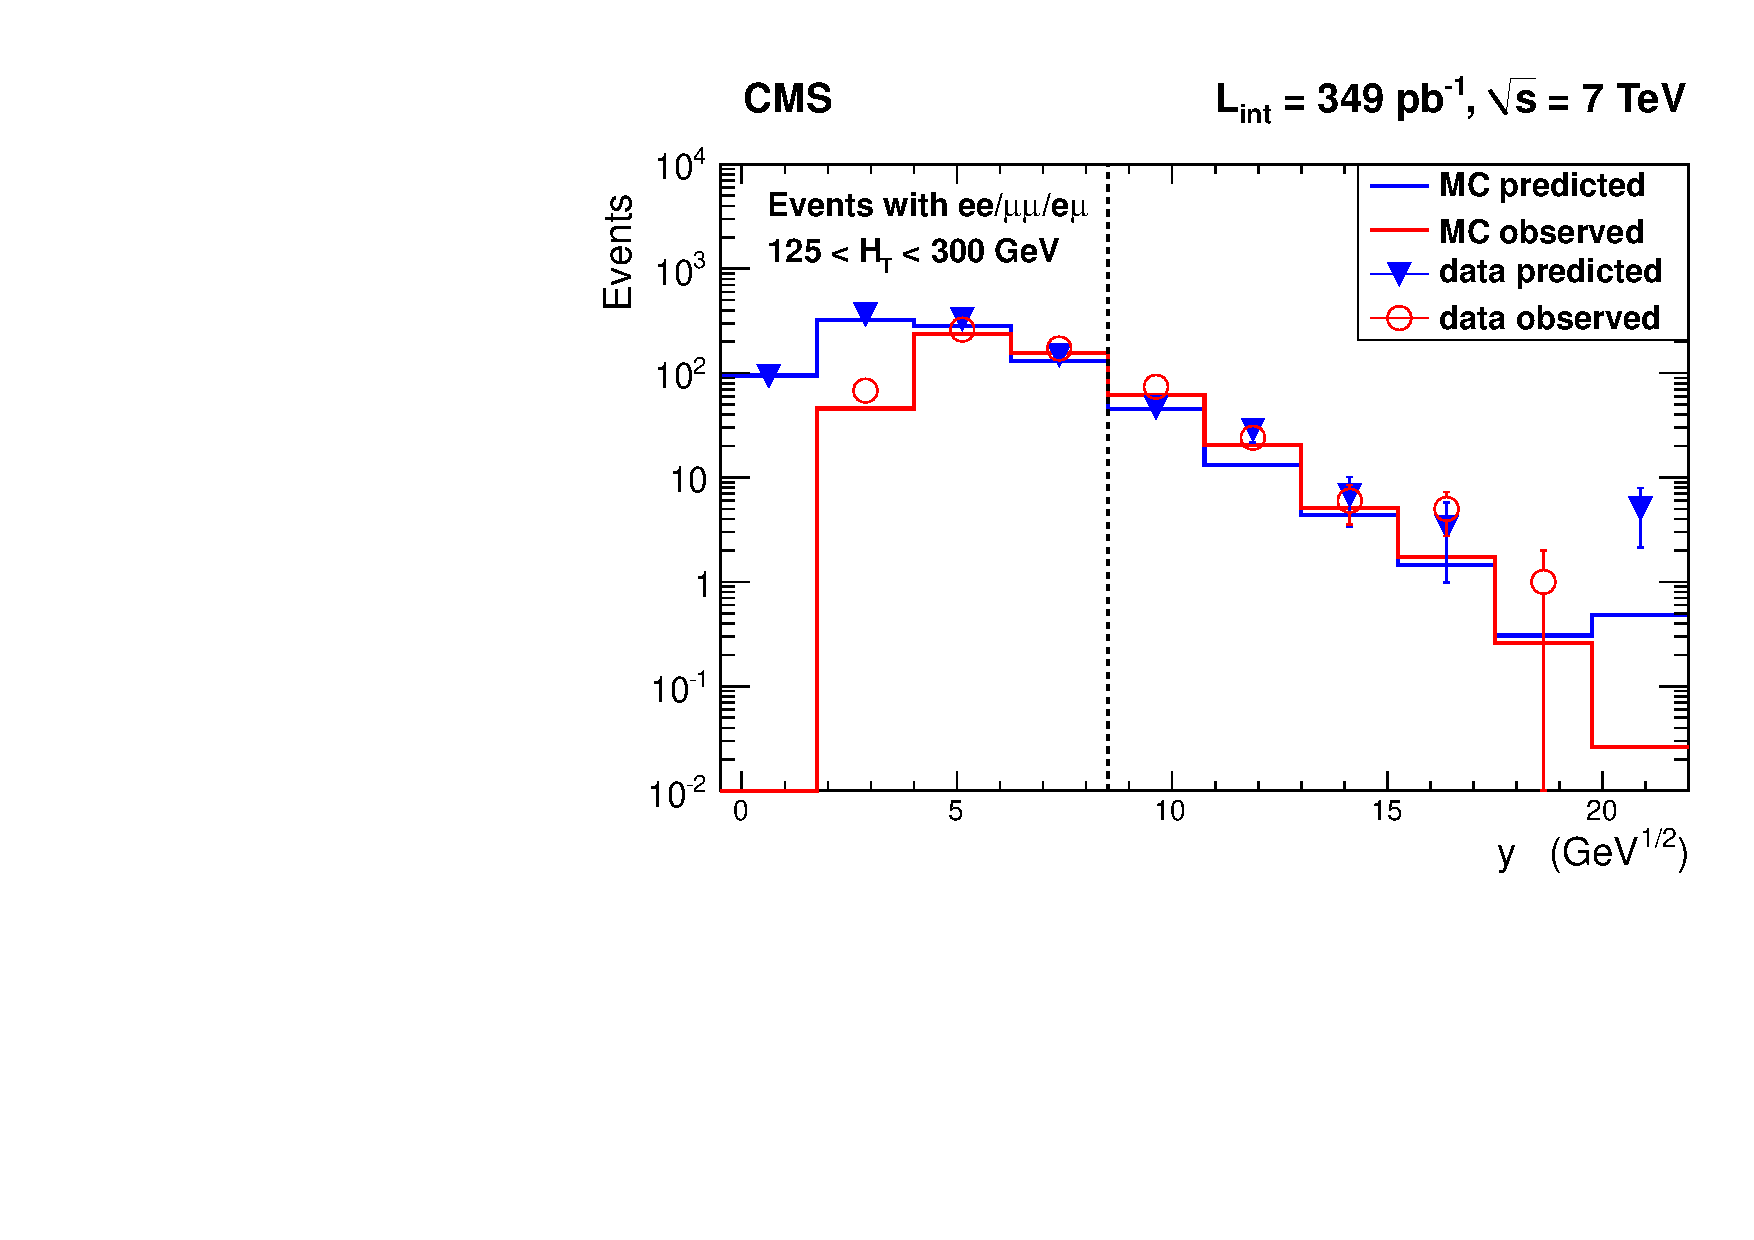
\includegraphics[width=0.48\linewidth]{plots/victory_y_control_349pb.pdf}
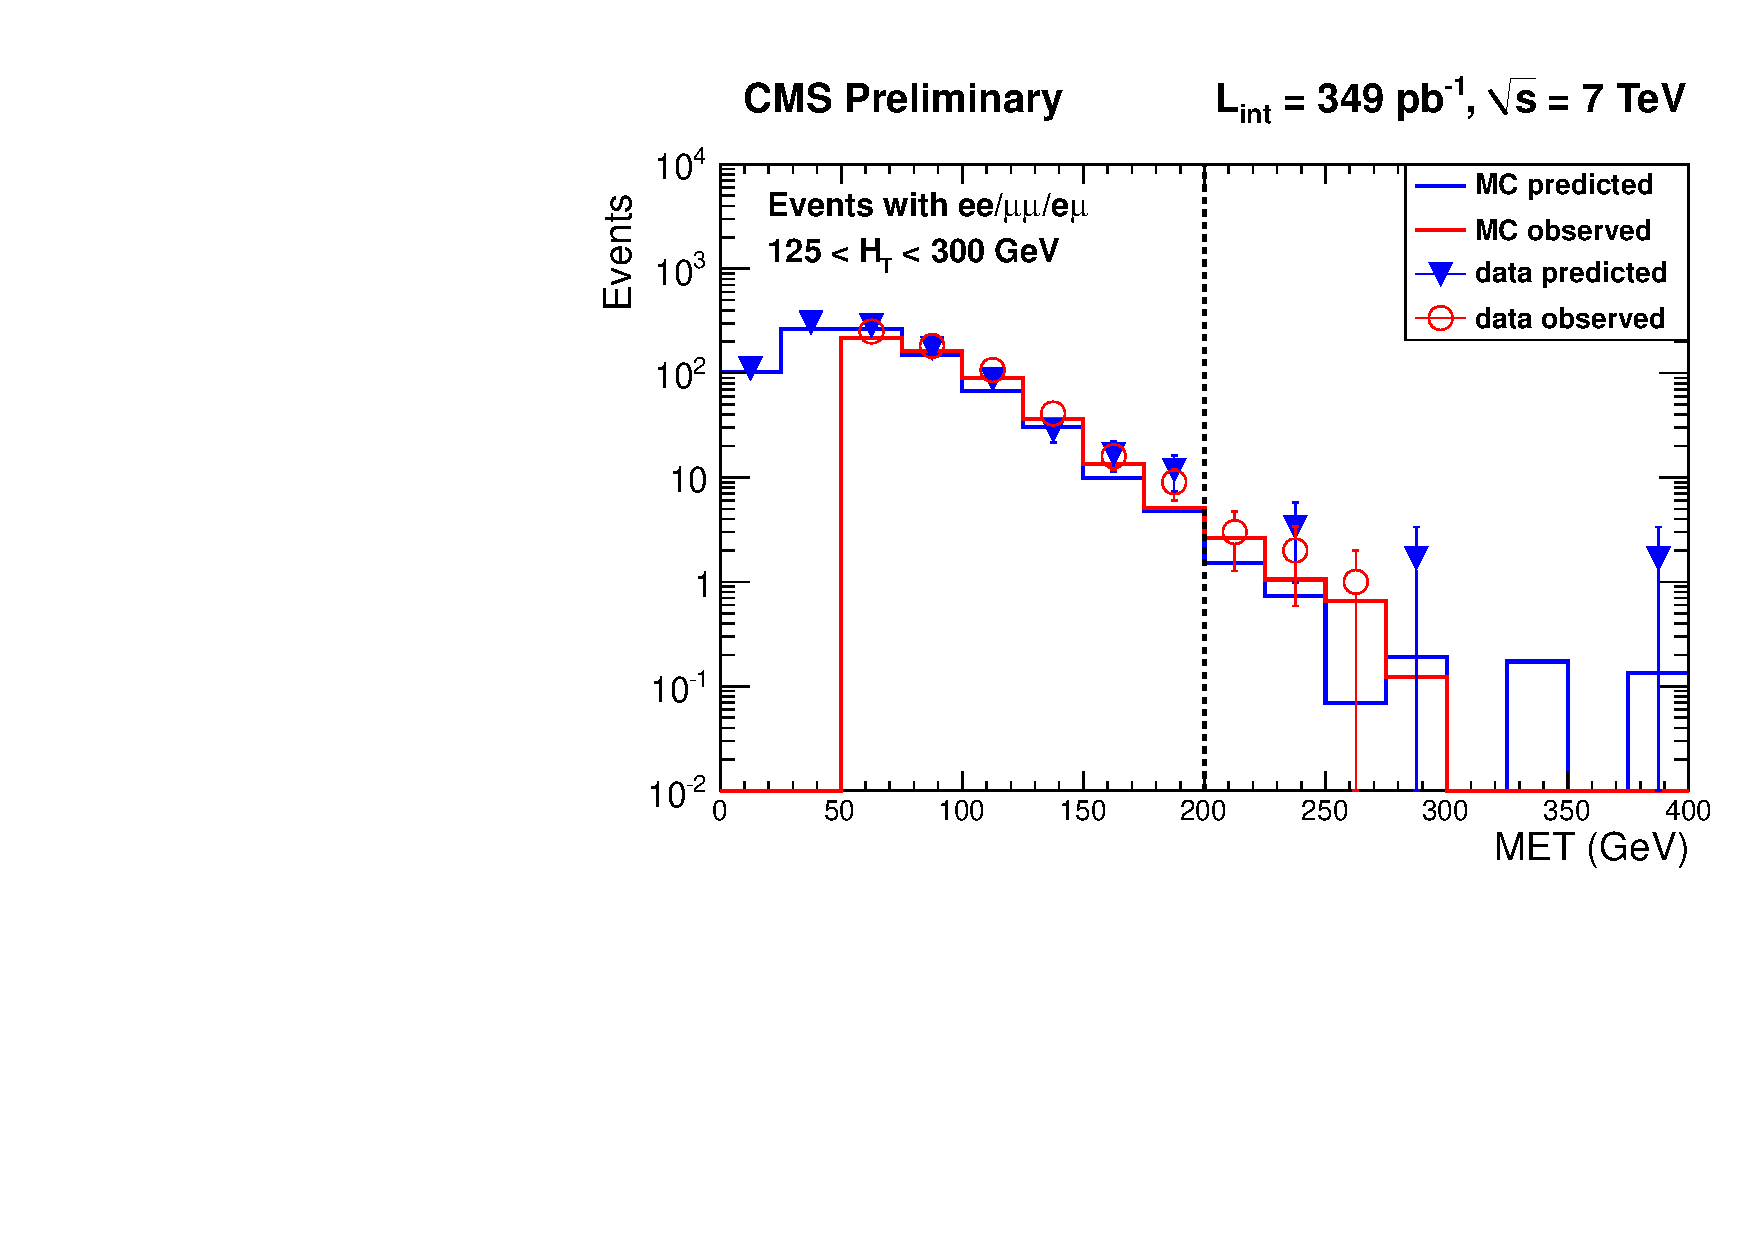
\includegraphics[width=0.48\linewidth]{plots/victory_met200_control_349pb.pdf}
\caption{\label{fig:victorycontrol}\protect 
Results of the \ptll\ method in the \Ht\ sideband region 125-300 GeV.
Left:  distributions of $\ptll/\sqrt{H_T}$ (predicted) and $y$ (observed) for 
SM MC and data. The vertical dashed lines indicate the requirement $y > 8.5$~GeV$^{1/2}$),
corresponding to the 2010 signal region.
Right: distributions of \ptll\ (predicted) and \met\ (observed) for 
SM MC and data. The vertical dashed lines indicate the requirement \met\ $>$ 200 GeV,
corresponding to the high \Ht\ signal region.
}
\end{center}
\end{figure}


\begin{figure}[tbh]
\begin{center}
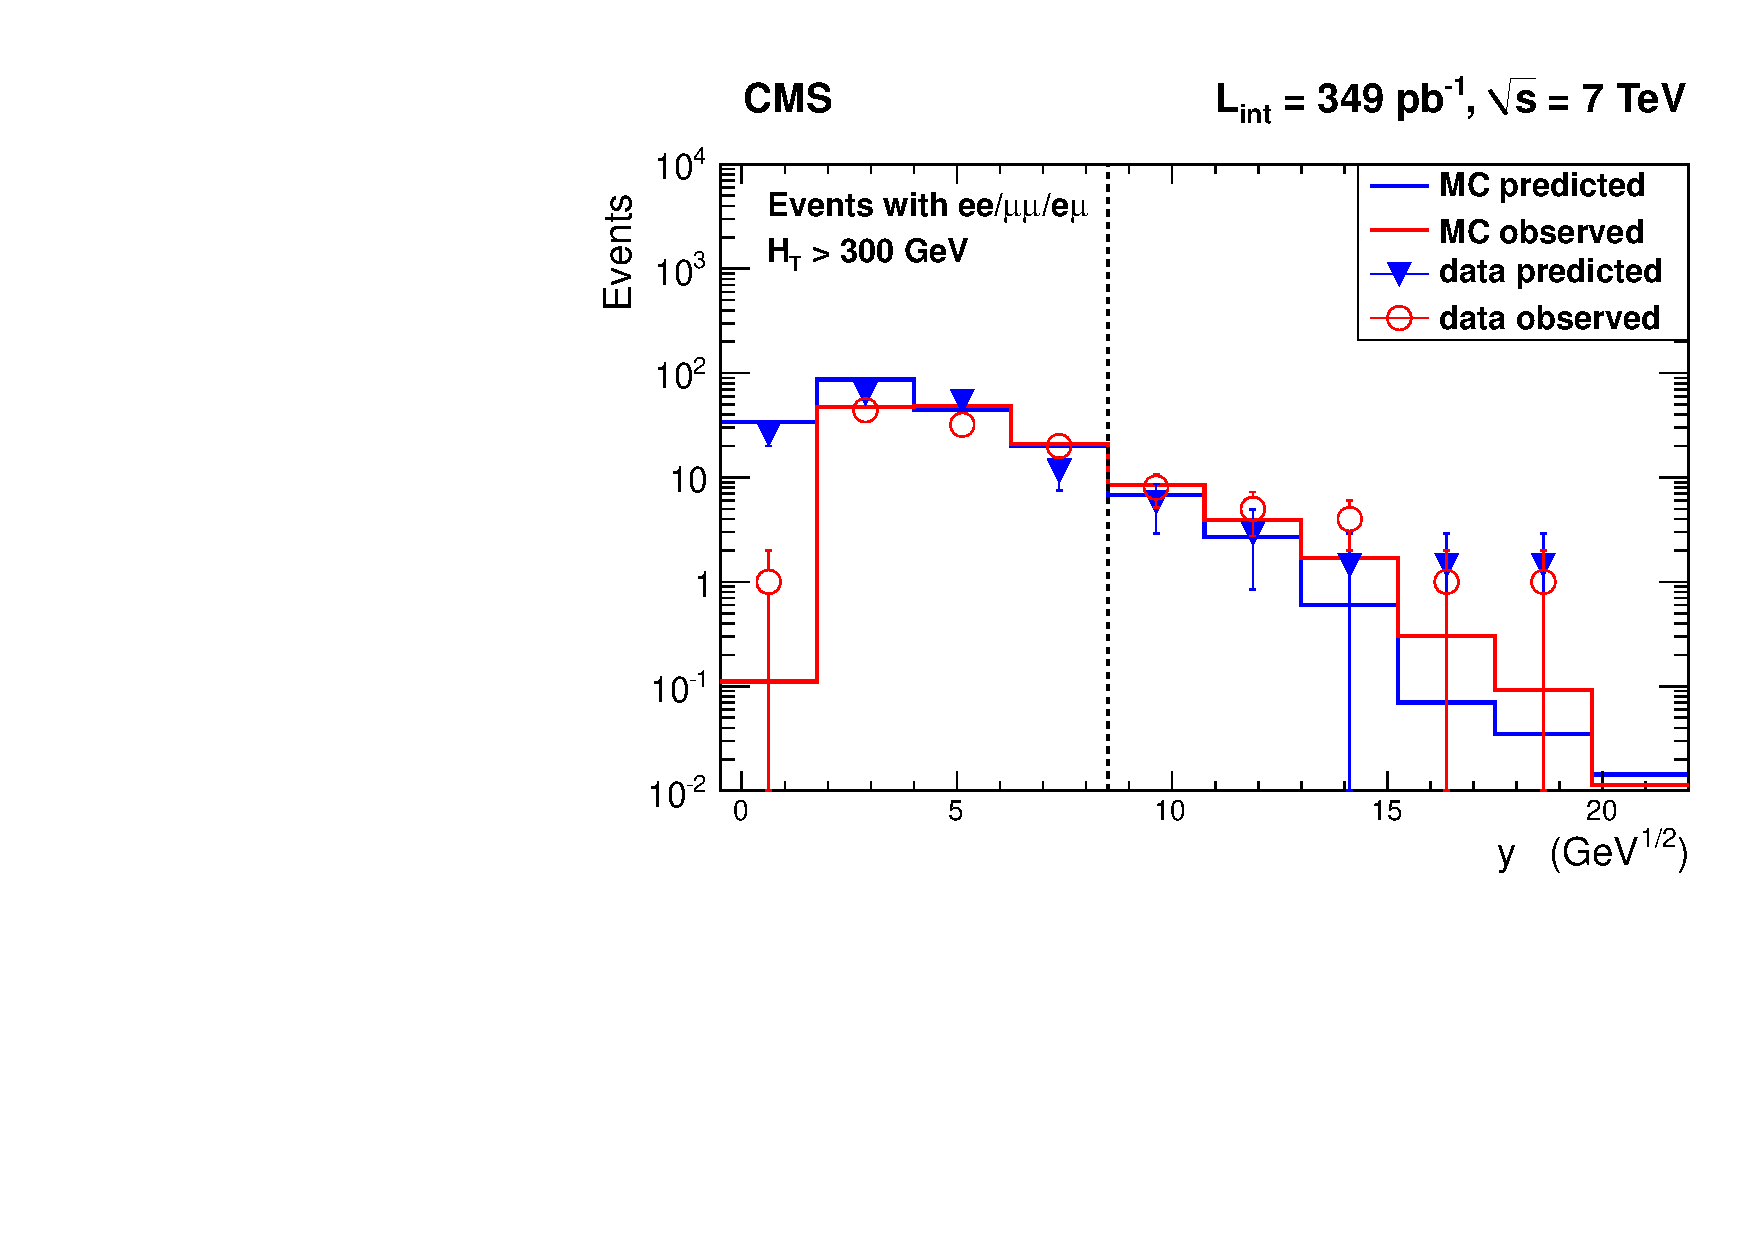
\includegraphics[width=0.6\linewidth]{plots/victory_y_ht300_349pb.pdf}
\caption{\label{fig:vic1}\protect 
Distributions of $\ptll/\sqrt{H_T}$ (predicted) and $y$ (observed) for 
SM MC and data, for the \Ht $>$ 300 GeV. 
The vertical dashed lines indicate the requirement $y > 8.5$~GeV$^{1/2}$ corresponding to the 2010 signal region.
}
\end{center}
\end{figure}

\begin{figure}[tbh]
\begin{center}
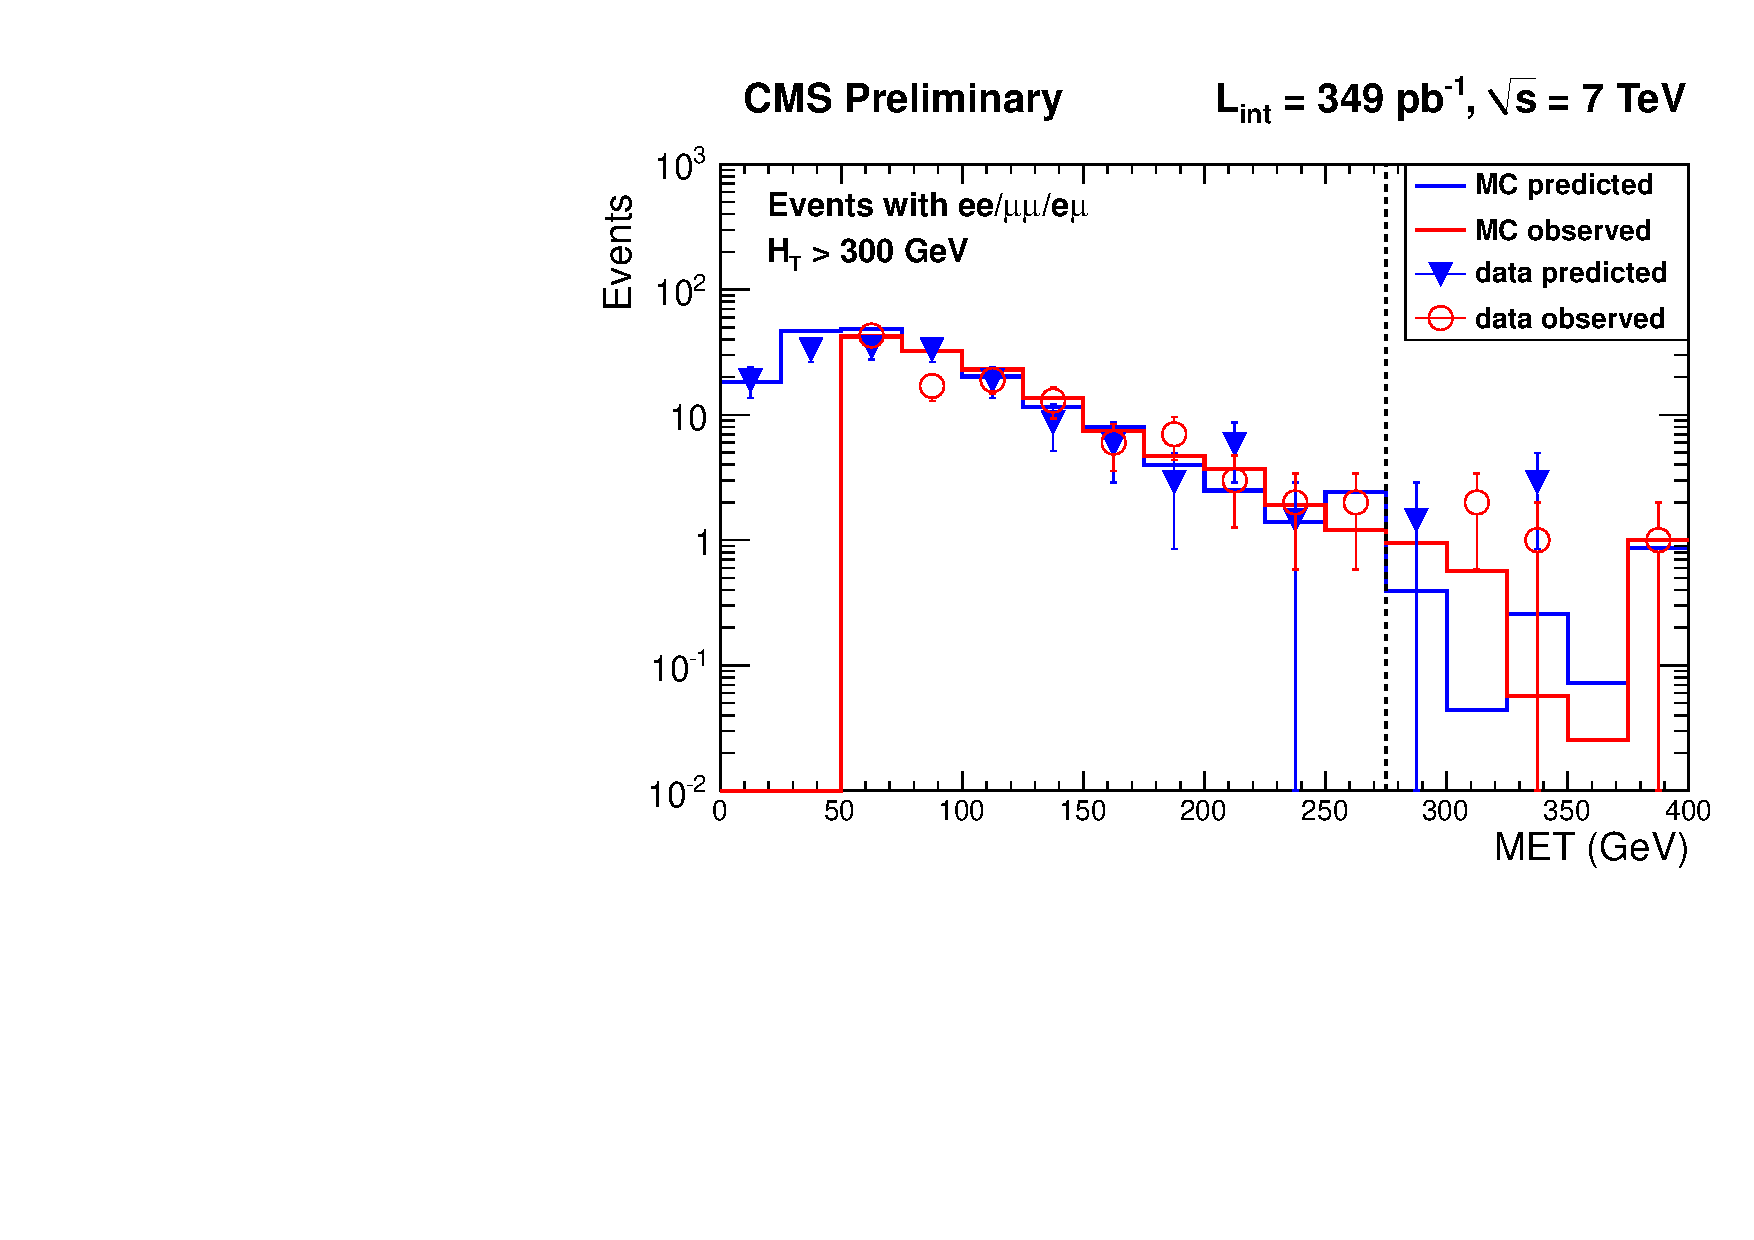
\includegraphics[width=0.6\linewidth]{plots/victory_met275_ht300_349pb.pdf}
\caption{\label{fig:v2}\protect 
Distributions of \ptll\ (predicted) and \met\ (observed) for 
SM MC and data, for the region \Ht $>$ 300 GeV. 
The vertical dashed lines indicate the requirement \met\ $>$ 275 GeV, corresponding to the high \met\ signal region.
}
\end{center}
\end{figure}

\begin{figure}[tbh]
\begin{center}
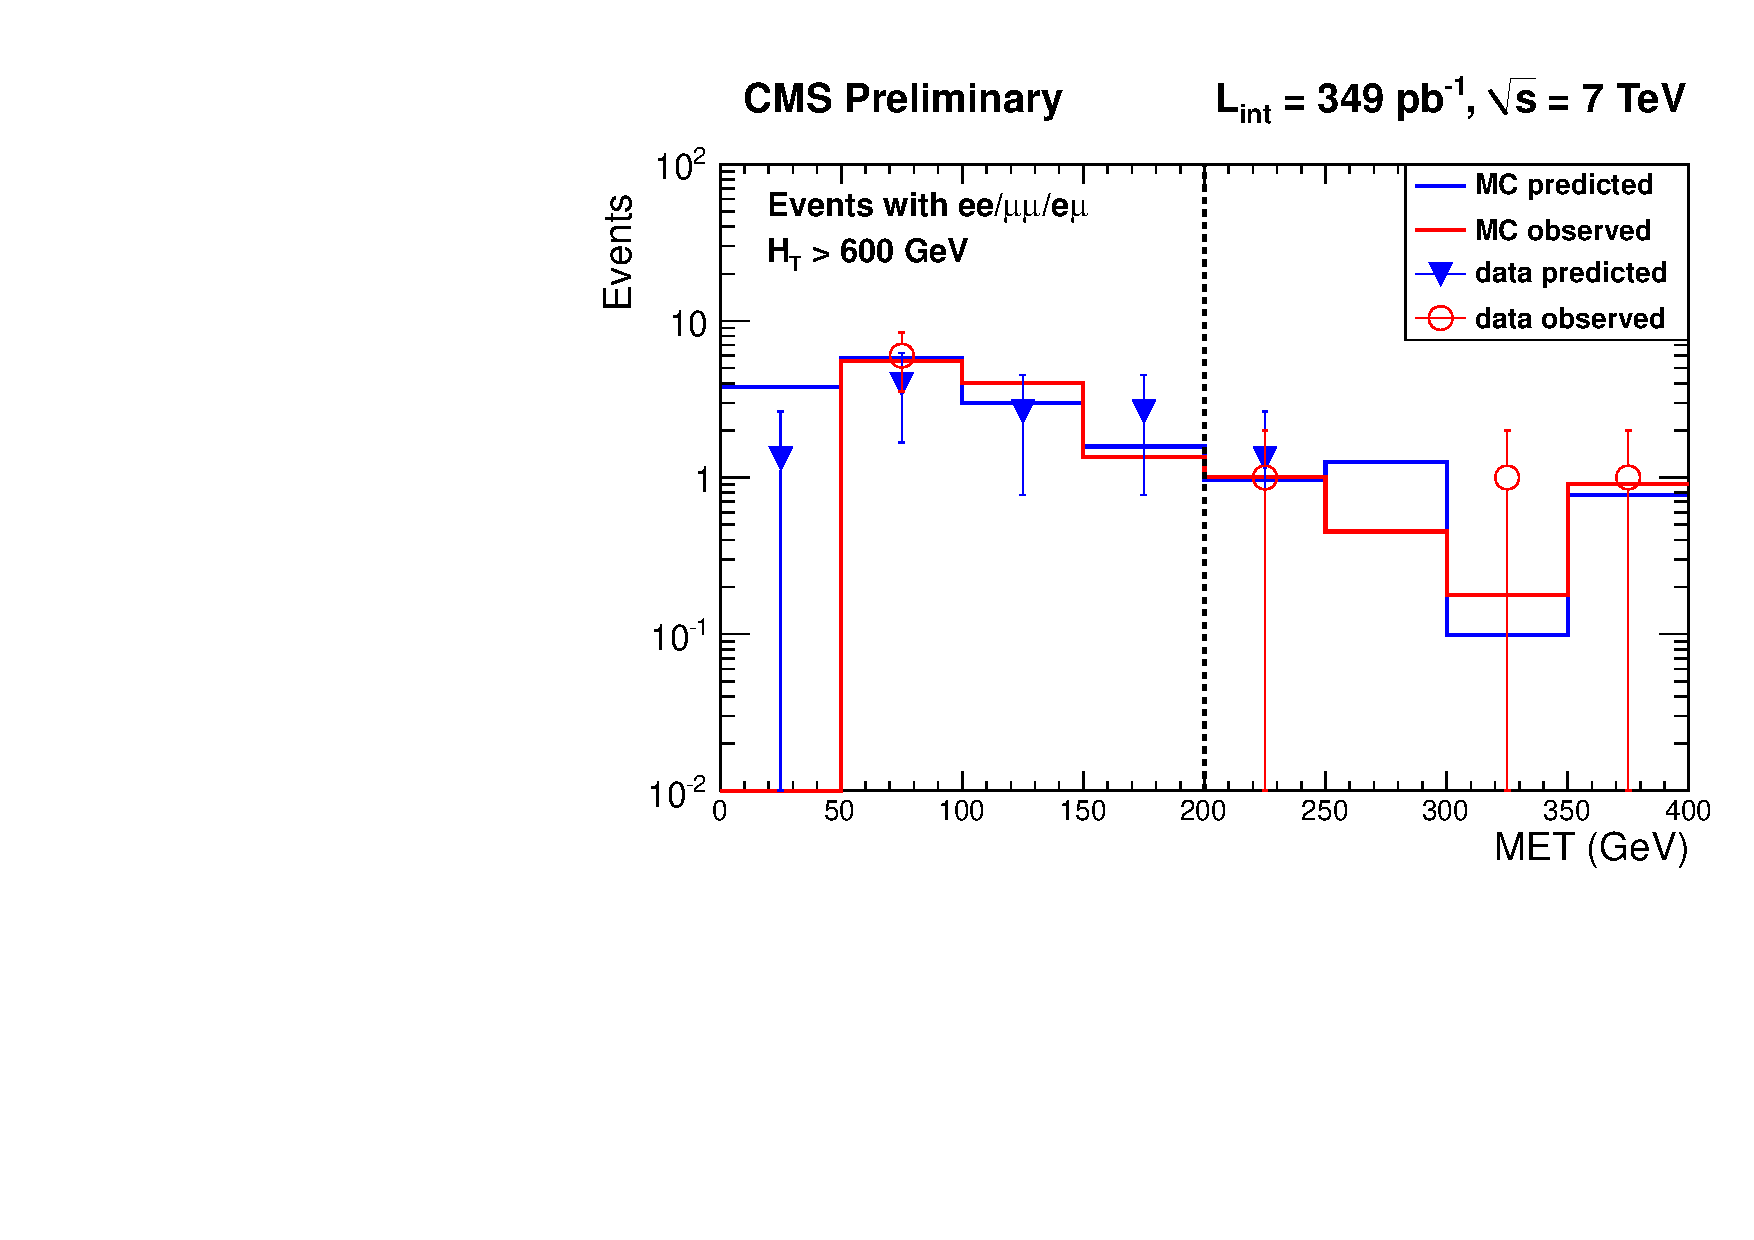
\includegraphics[width=0.6\linewidth]{plots/victory_met200_ht600_349pb.pdf}
\caption{\label{fig:vic3}\protect 
Distributions of \ptll\ (predicted) and \met\ (observed) for 
SM MC and data, for the region \Ht $>$ 600 GeV. 
The vertical dashed lines indicate the requirement \met\ $>$ 200 GeV, corresponding to the high \Ht\ signal region.
}
\end{center}
\end{figure}

\subsection{Background estimate from OF subtraction}
\label{sec:ofres}

The results of the OF subtraction technique applied to the high \pt\ dilepton trigger sample are summarized in Table~\ref{tab:ofres}. 
We evaluate the quantity $\Delta = R_{\mu e}N(ee) + \frac{1}{R_{\mu e}}N(\mu\mu) - N(e\mu)$ with $R_{\mu e} = 1.12 \pm 0.05$
extracted from the ratio of $Z \to \mu^+\mu^-$ vs. $Z \to e^+e^-$ events in data.
We perform the OF subtraction first in the preselection region, and find $\Delta$ consistent with 0, as expected.
We then perform the OF subtraction in all 3 signal regions, and do not observe any excess of same-flavor vs. opposite-flavor events.

\begin{table}[hbt]
\begin{center}
\caption{\label{tab:ofres} Summary of results for the OF subtraction technique. 
The quantity $\Delta = R_{\mu e}N(ee) + \frac{1}{R_{\mu e}}N(\mu\mu) - N(e\mu)$ is quoted with $R_{\mu e} = 1.12 \pm 0.05$.
The quoted systematic uncertainty corresponds to that of $R_{\mu e}$. The $e\mu$ yields differ from those previously
quoted because the $Z$ mass veto is included here.
}
\begin{tabular}{l|ccc|c}
\hline
region                   &  $N(ee)$ & $N(\mu\mu)$ & $N(e\mu)$  &  $\Delta$   \\ 
\hline
preselection region      &      193 &         201 &      394   &    2.0 $\pm$ 28 (stat) $\pm$ 1.8 (syst) \\    
2010 signal region       &        4 &           4 &        9   &   -0.9 $\pm$ 4.2 (stat) $\pm$ 0.1 (syst)  \\
high \met\ signal region &        2 &           0 &        1   &    1.3 $\pm$ 1.9 (stat) $\pm$ 0.1 (syst)  \\
high \Ht\ signal region  &        1 &           0 &        1   &    0.1 $\pm$ 1.5 (stat) $\pm$ 0.0 (syst)  \\
\hline
\end{tabular}
\end{center}
\end{table}

For the dilepton-\Ht\ trigger sample, we observe only 1 event in the 2010 signal region, consistent with MC expectations,
and no events in either the high $y$ or high \Ht\ signal regions. In the case of an excess of events at low lepton \pt,
we will perform the OF subtraction technique of Sec.~\ref{sec:oflowpt}.

% \clearpage
\subsection{Summary of results}

\begin{table}[hbt]
\begin{center}
\caption{\label{tab:results} 
Summary of the observed and predicted yields in the 3 signal regions. MC errors are statistical only. The systematic uncertainty on the ABCD
and \ptll\ method is from the scaling factors from MC closure only. 
%{\bf need to put additional uncertainties, for example jet/met scale.}
For the OF subtraction, the quantity $\Delta = R_{\mu e}N(ee) + \frac{1}{R_{\mu e}}N(\mu\mu) - N(e\mu)$ is quoted; the systematic uncertainty
here is from the ratio of muon to electron selection efficiencies.
}
\begin{tabular}{l|c|c|c}
\hline
                                       &  2010 signal region                       &   high \met\ signal region             &  high \Ht\ signal region              \\ 
\hline
Observed yield                         &         19                                &                        4               &                        3              \\
\hline
MC prediction                          &    14.5 $\pm$ 1.4                         &            2.6 $\pm$ 0.8               &            2.5 $\pm$ 0.8              \\
ABCD prediction                        &    12.7 $\pm$ 2.4 (stat) $\pm$ 2.5 (syst) &                                        &                                       \\
ABCD' prediction                       &    12.8 $\pm$ 2.9 (stat) $\pm$ 2.6 (syst) & 1.2 $\pm$ 0.4 (stat) $\pm$ 0.5 (syst)  & 0.0 $\pm$ 0.6 (stat) $\pm$ 0.3 (syst) \\
\ptll\ prediction                      &    16.7 $\pm$ 6.1 (stat) $\pm$ 5.9 (syst) & 5.4 $\pm$ 3.8 (stat) $\pm$ 2.2 (syst)  & 1.7 $\pm$ 1.7 (stat) $\pm$ 0.6 (syst) \\
\hline
OF subtraction ($\Delta$)              &    -0.9 $\pm$ 4.2 (stat) $\pm$ 0.1 (syst) & 1.3 $\pm$ 1.9 (stat) $\pm$ 0.1 (syst)  & 0.1 $\pm$ 1.5 (stat) $\pm$ 0.0 (syst) \\
\hline
\end{tabular}
\end{center}
\end{table}

A summary of our results is presented in Table~\ref{tab:results}. In all 3 signal regions, we observe reasonable agreement
between the observed yields and the predictions from MC and data-driven background estimates. We therefore do not observe
evidence for an excess of events above SM expectations. After assessing systematic uncertainties in Sec.~\ref{sec:systematics},
we proceed to set upper limits on the non-SM contributions to the signal regions in Sec.~\ref{sec:limits}.

\clearpage

%syst on bkgnd preds
\section{Systematics Uncertainties in the Background Prediction}
\label{sec:systematics}

The methodology for determining the systematics on the background
predictions has not changed with respect to the nominal analysis.
Because the template method has not changed, the same 
systematic uncertainty is assessed on this prediction (32\%).
The 50\% uncertainty on the WZ and ZZ background is also unchanged.
The systematic uncertainty in the OF background prediction based on 
e$\mu$ events has changed, due to the different composition of this
sample after vetoing events containing b-tagged jets.

As in the nominal analysis, we do not require the e$\mu$ events
to satisfy the dilepton mass requirement and apply a scaling factor K,
extracted from MC, to account for the fraction of e$\mu$ events
which satisfy the dilepton mass requirement. This procedure is used
in order to improve the statistical precision of the OF background estimate.

For the selection used in the nominal analysis, 
the e$\mu$ sample is completely dominated by $t\bar{t}$
events, and we observe that K is statistically consistent with constant with
respect to the \MET\ requirement. However, in this analysis, the $t\bar{t}$
background is strongly suppressed by the b-veto, and hence the non-$t\bar{t}$
backgrounds (specifically, $Z\to\tau\tau$ and VV) become more relevant. 
At low \MET, the $Z\to\tau\tau$ background is pronounced, while $t\bar{t}$
and VV dominate at high \MET\ (see App.~\ref{app:kinemu}).
Therefore, the sample composition changes
as the \MET\ requirement is varied, and as a result K depends
on the \MET\ requirement. 

We thus measure K in MC separately for each
\MET\ requirement, as displayed in Fig.~\ref{fig:kvmet} (left).
%The systematic uncertainty on K is determined separately for each \MET\
%requirement by comparing the relative difference in K in data vs. MC.
The values of K used are the MC predictions 
%and the total systematic uncertainty on the OF prediction 
%as shown in 
(Table \ref{fig:kvmettable}).
The contribution to the total OF prediction systematic uncertainty 
from K is assessed from the ratio of K in data and MC,
shown in Fig.~\ref{fig:kvmet} (right).
The ratio is consistent with unity to roughly 17\%, 
so we take this value as the systematic from K.
17\% added in quadrature with 7\% from 
the electron to muon efficieny ratio 
(as assessed in the inclusive analysis)
yields a total systematic of $\sim$18\% 
which we round up to 20\%.
For \MET\ $>$ 150, there are no OF events in data inside the Z mass window
so we take a systematic based on the statistical uncertainty
of the MC prediction for K. 
This value is 25\% for \MET\ $>$ 150 GeV and 60\% for \MET\ $>$ 200 GeV.
%Although we cannot check the value of K in data for \MET\ $>$ 150
%because we find no OF events inside the Z mass window for this \MET\ 
%cut, the overall OF yields with no dilepton mass requirement 
%agree to roughly 20\% (9 data vs 7.0 $\pm$ 1.1 MC).


%Below Old

%In reevaluating the systematics on the OF prediction, however,
%we observed a different behavior of K as a function of \MET\ 
%as was seen in the inclusive analysis. 

%Recall that K is the ratio of the number of \emu\ events
%inside the Z window to the total number of \emu\ events.
%In the inclusive analysis, it is taken from \ttbar\ MC
%and used to scale the inclusive \emu\ yield in data.
%The yield scaled by K is then corrected for 
%the $e$ vs $\mu$ efficiency difference to obtain the 
%final OF prediction.

%Based on the plot in figure \ref{fig:kvmet}, 
%we choose to use a different
%K for each \MET\ cut and assess a systematic uncertainty
%on the OF prediction based on the difference between 
%K in data and MC. 
%The variation of K as a function of \MET\ is caused 
%by a change in sample composition with increasing \MET.
%At \MET\ $<$ 60 GeV, the contribution of Z plus jets is
%not negligible (as it was in the inclusive analysis)
%because of the b veto. (See appendix \ref{app:kinemu}.)
%At higher \MET, \ttbar\ and diboson backgrounds dominate.




\begin{figure}[hbt]
  \begin{center}
	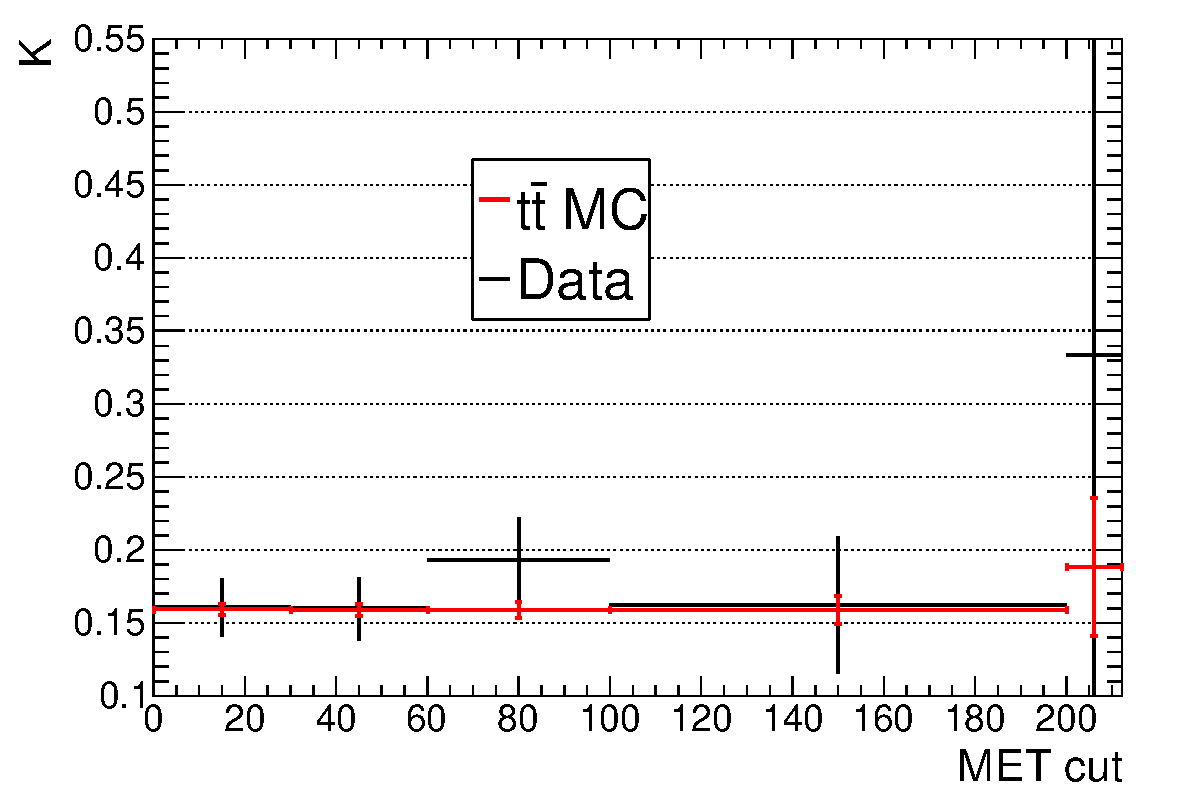
\includegraphics[width=0.48\linewidth]{plots/kvmet_data_ttbm.pdf}
	\includegraphics[width=0.48\linewidth]{plots/kvmet_ratio.pdf}
	\caption{
	  \label{fig:kvmet}\protect 
	  The left plot shows
	  K as a function of \MET\ in MC (red) and data (black). 
	  The bin low edge corresponds to the \MET\ cut, and the 
	  bins are inclusive.
	  The MC used is a sum of all SM MC used in the yield table of
	  section \ref{sec:yields}.
	  The right plot is the ratio of K in data to MC.
	  The ratio is fit to a line whose slope is consistent with zero
	  (the fit parameters are 
	  0.9 $\pm$  0.4 for the intercept and
      0.001 $\pm$ 0.005 for the slope).
	}
  \end{center}
\end{figure}



\begin{table}[htb]
\begin{center}
\caption{\label{fig:kvmettable} The values of K used in the OF background prediction. 
The uncertainties shown are the total relative systematic used for the OF prediction,
which is the systematic uncertainty from K added in quadrature with
a 7\% uncertainty from the electron to muon efficieny ratio as assessed in the
inclusive analysis.
}
\begin{tabular}{lcc}
\hline
\MET\ Cut    &    K        &  Relative Systematic \\
\hline
%the met zero row is used only for normalization of the money plot.
%0    &  0.1   &        \\  
30   &  0.12  &  20\%  \\  
60   &  0.13  &  20\%  \\  
80   &  0.12  &  20\%  \\  
100  &  0.12  &  20\%  \\  
150  &  0.09  &  25\%  \\  
200  &  0.06  &  60\%  \\  
\hline
\end{tabular}
\end{center}
\end{table}


%UL on non-SM yeild
\section{Upper Limit on Non SM Yield}
\label{sec:upperlimit}

The results of summing the predicted backgrounds from the MET templates and OF subtraction
methods are shown in table \ref{tab:systrestot}.


\begin{table}[hbt]
  \begin{center}
	\caption{
	  \label{tab:systrestot}
	  Combination of predictions from MET templates and OF subtraction.
	}
	\begin{tabular}{lcccc}
	  \hline
	  \resulttitle
\hline

Prediction & 460.97 $\pm$ 7.69 $\pm$ 101.57  &    47.86 $\pm$ 2.66 $\pm$ 3.51  &    13.16 $\pm$ 1.50 $\pm$ 0.55  &     1.18 $\pm$ 0.46 $\pm$ 0.04  \\

\hline
	\end{tabular}
  \end{center}
\end{table}


%loose signal region:  6.04 $\pm$ 0.82 (stat) $\pm$ 0.51 (syst)  \\
%tight signal region:  1.24 $\pm$ 0.42 (stat) $\pm$ 0.07 (syst).

Using the results of the background predictions shown in table \ref{tab:systrestot},
we calculate the Bayesian 95\% CL
upper limits on the non SM event yields (Gaussian nuissance parameter model) shown in 
table \ref{tab:modinul}.

\begin{table}[hbt]
  \begin{center}
	\caption{
	  \label{tab:modinul}
	  Model independent upper limit (UL) on non-SM event yields.
	}
	\begin{tabular}{lcccc}
	  \hline
	  \resulttitle
\hline

Prediction & 460.97 $\pm$ 101.86  &    47.86 $\pm$ 4.40  &    13.16 $\pm$ 1.60  &     1.18 $\pm$ 0.46 \\

Data      &                488  &                   39  &                   14  &                    2  \\
\hline
{\bf UL}        &224.85  &  11.95  &  10.22  &  5.38\\


\hline
	\end{tabular}
  \end{center}
\end{table}

%2010 results
%loose signal region: $N_{BG} = 6.04 \pm 0.96$, $N_{OBS} = 7 \rightarrow$ {\bf UL = 7.9 events} \\
%tight signal region: $N_{BG} = 1.24 \pm 0.43$, $N_{OBS} = 0 \rightarrow$ {\bf UL = 3.0 events} \\


%Additional Information for Model Testing
\section{Outreach}
\label{sec:outreach}
Conveying additional useful information about the results of
a generic ``signature-based'' search such as the one described
in this note is a difficult issue.  
Here we attempt to present our result in the most general 
way.

Models of new physics in the dilepton final state 
can be confronted in an approximate way by simple 
generator-level studies that 
compare the expected number of events in \lumi\
with our upper limits in Sec.~\ref{sec:limits}.  The key ingredients
of such studies are the kinematical cuts described 
in this note, the lepton efficiencies, and the detector
responses for \Ht, $y$, and \met.

The muon identification efficiency is $\approx 96\%$;
the electron identification efficiency varies approximately linearly from $\approx$ 60\% at 
\pt = 10 GeV to 90\% for \pt $>$ 30 GeV.  
%
The lepton isolation efficiency depends on the lepton momentum, as well as on the jet activity in the 
event.
In $t\bar{t}$ events, it varies approximately linearly from $\approx 73\%$ (muons)
and $\approx 82\%$ (electrons) at \pt = 10 GeV to $\approx 97\%$ for \pt $>$ 60 GeV. 
In LM1 (LM3,LM6) events, this efficiency is decreased by $\approx$5--10\% ($\approx$10\%,$\approx$5\%)over the whole momentum spectrum.
%
The average detector responses (the reconstructed quantity divided by the generated quantity) 
for \Ht, $y$ and \met\ are consistent with 1 within the 5\% jet energy scale uncertainty.
The experimental resolutions on these quantities are 9\%, 12\% and 12\%, respectively.

To justify the statements in the previous paragraph 
about the detector responses, we plot 
in Figure~\ref{fig:response} the average response for 
\Ht, $y$ and \met, as well as the
efficiency for the cuts on these quantities used in defining the
signal region.

The lepton identification and isolation efficiencies are displayed for the dominant
\ttbar\ background in Fig.~\ref{fig:leptoneff}. The isolation efficiencies for the LM1
and LM3 processes are displayed in Fig.~\ref{fig:leptoniso}, which shows the decrease
in isolation efficiency resulting from the large hadronic activity in these events.


%Using this information as well as the kinematical
%cuts described in Section~\ref{sec:eventSel} and the lepton efficiencies
%of Figures~\ref{fig:effttbar}, one should be able to confront
%any existing or future model via a relatively simple generator 
%level study by comparing the expected number of events in 35 pb$^{-1}$
%with our upper limit of 4.1 events.

\begin{figure}[tbh]
\begin{center}
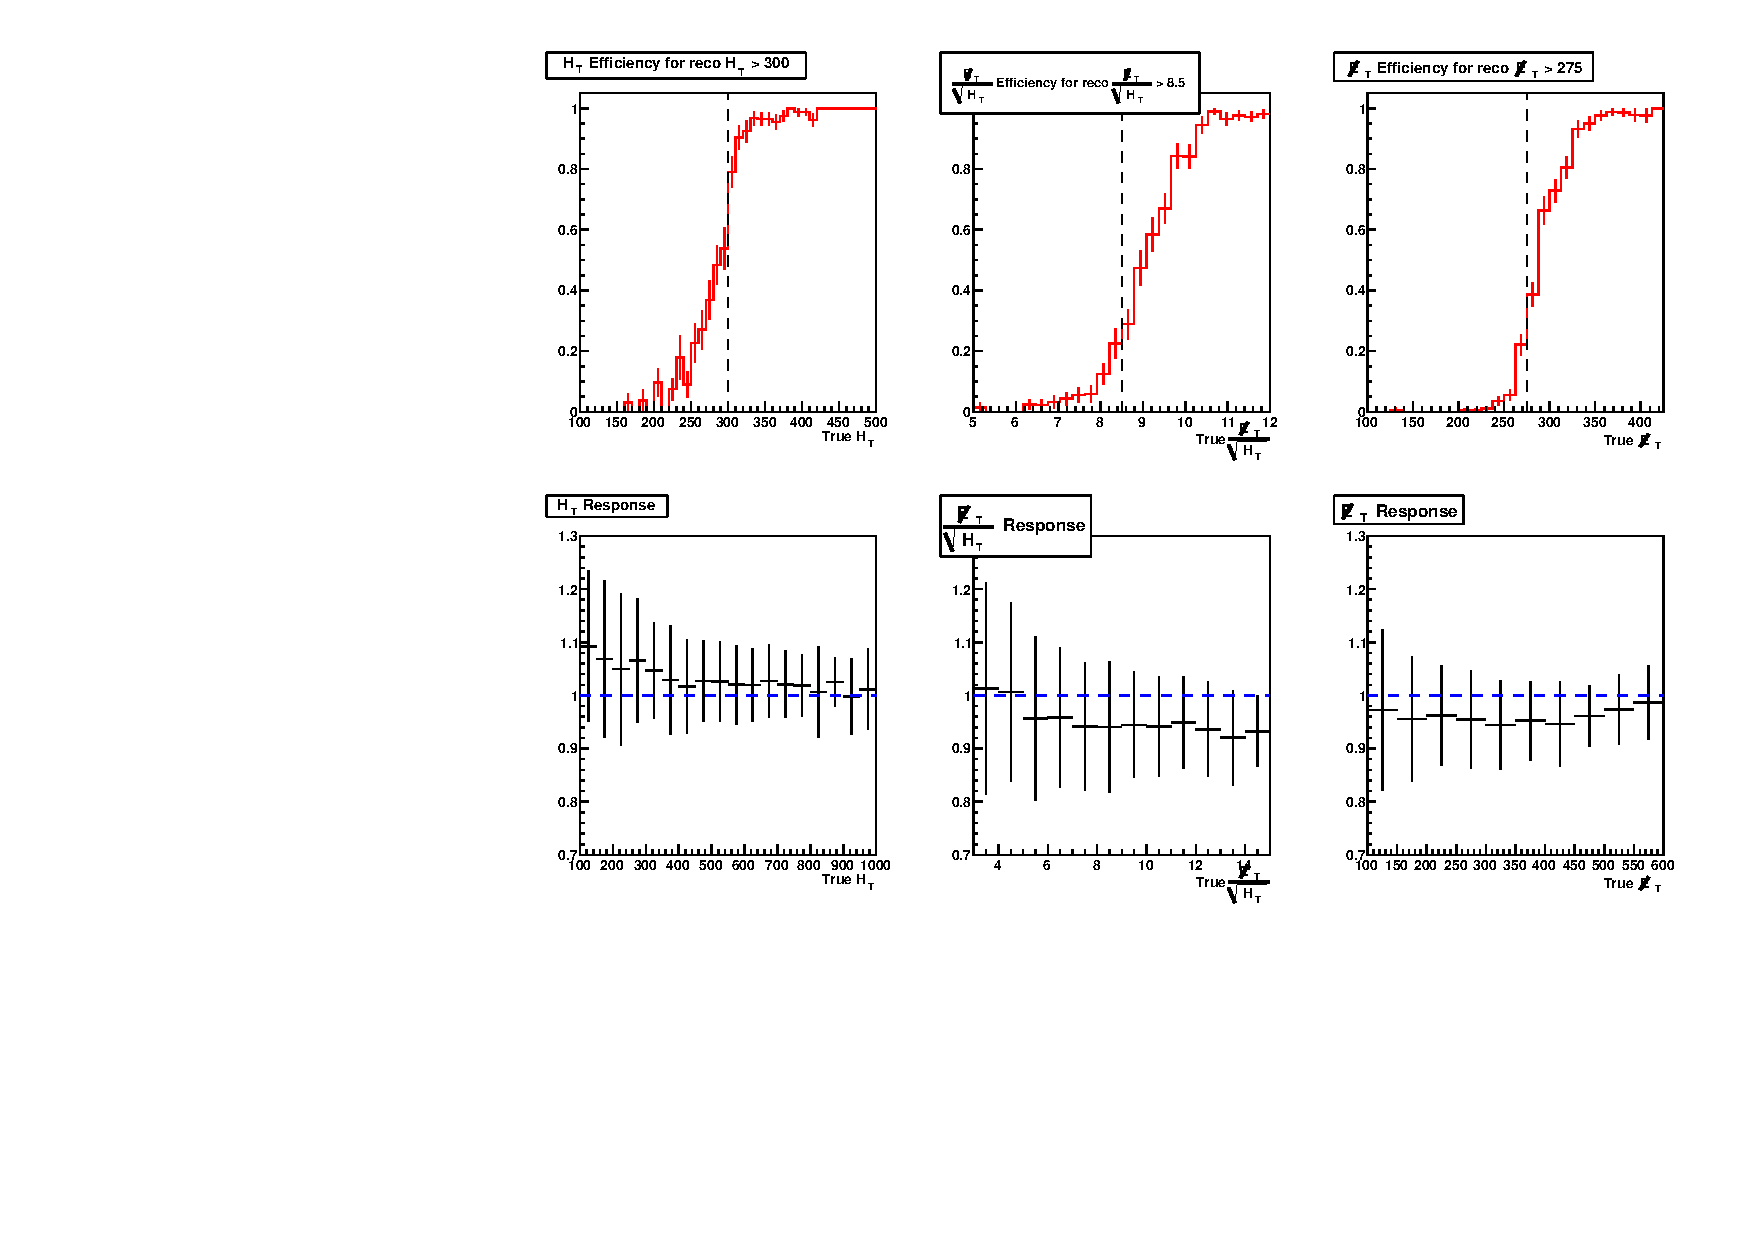
\includegraphics[width=\linewidth]{plots/lm1_SelectionEfficiency.pdf}
\caption{\label{fig:response} 
Top plots: the efficiencies to pass the signal region requirements (vertical dashed lines) on \Ht\ (left), $y$ (middle) and \met\ (right) as a function
of the generated quantities. Bottom plots: the average detector responses for \Ht, $y$ and \met\ and the corresponding RMS (error bars), as a function 
of the generated quantities. The response is defined as the ratio of the reconstructed quantity
to the true quantity in MC.  These plots are done using the LM1
Monte Carlo, but they are not expected to depend strongly on 
the underlying physics.
}
\end{center}
\end{figure}

\begin{figure}[tbh]
\begin{center}
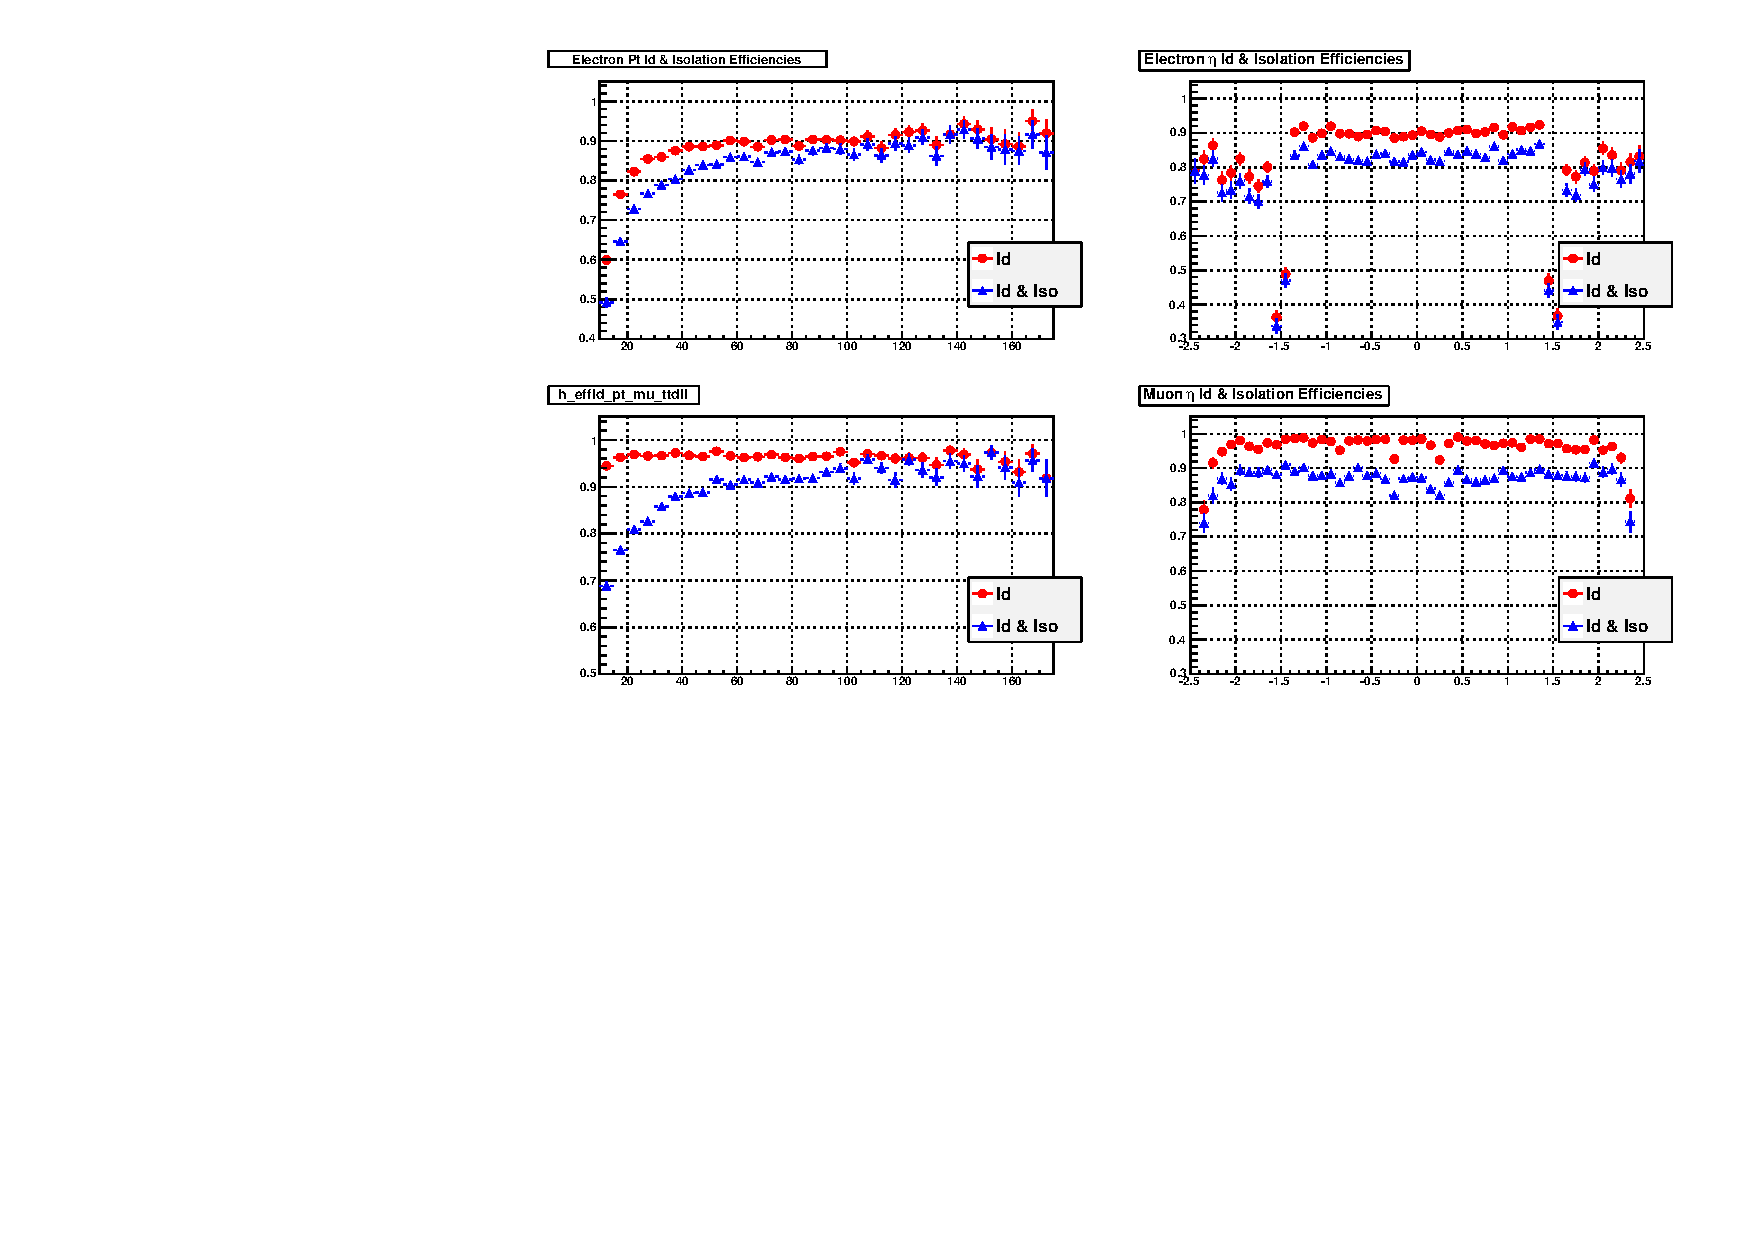
\includegraphics[width=\linewidth]{plots/ttdil_leptonEfficiencies.pdf}
\caption{\label{fig:leptoneff} 
The lepton identification and isolation efficiencies in \ttbar\ MC for electrons (top) and muons (bottom)
vs. \pt\ (left) and $\eta$ (right).
}
\end{center}
\end{figure}

\begin{figure}[tbh]
\begin{center}
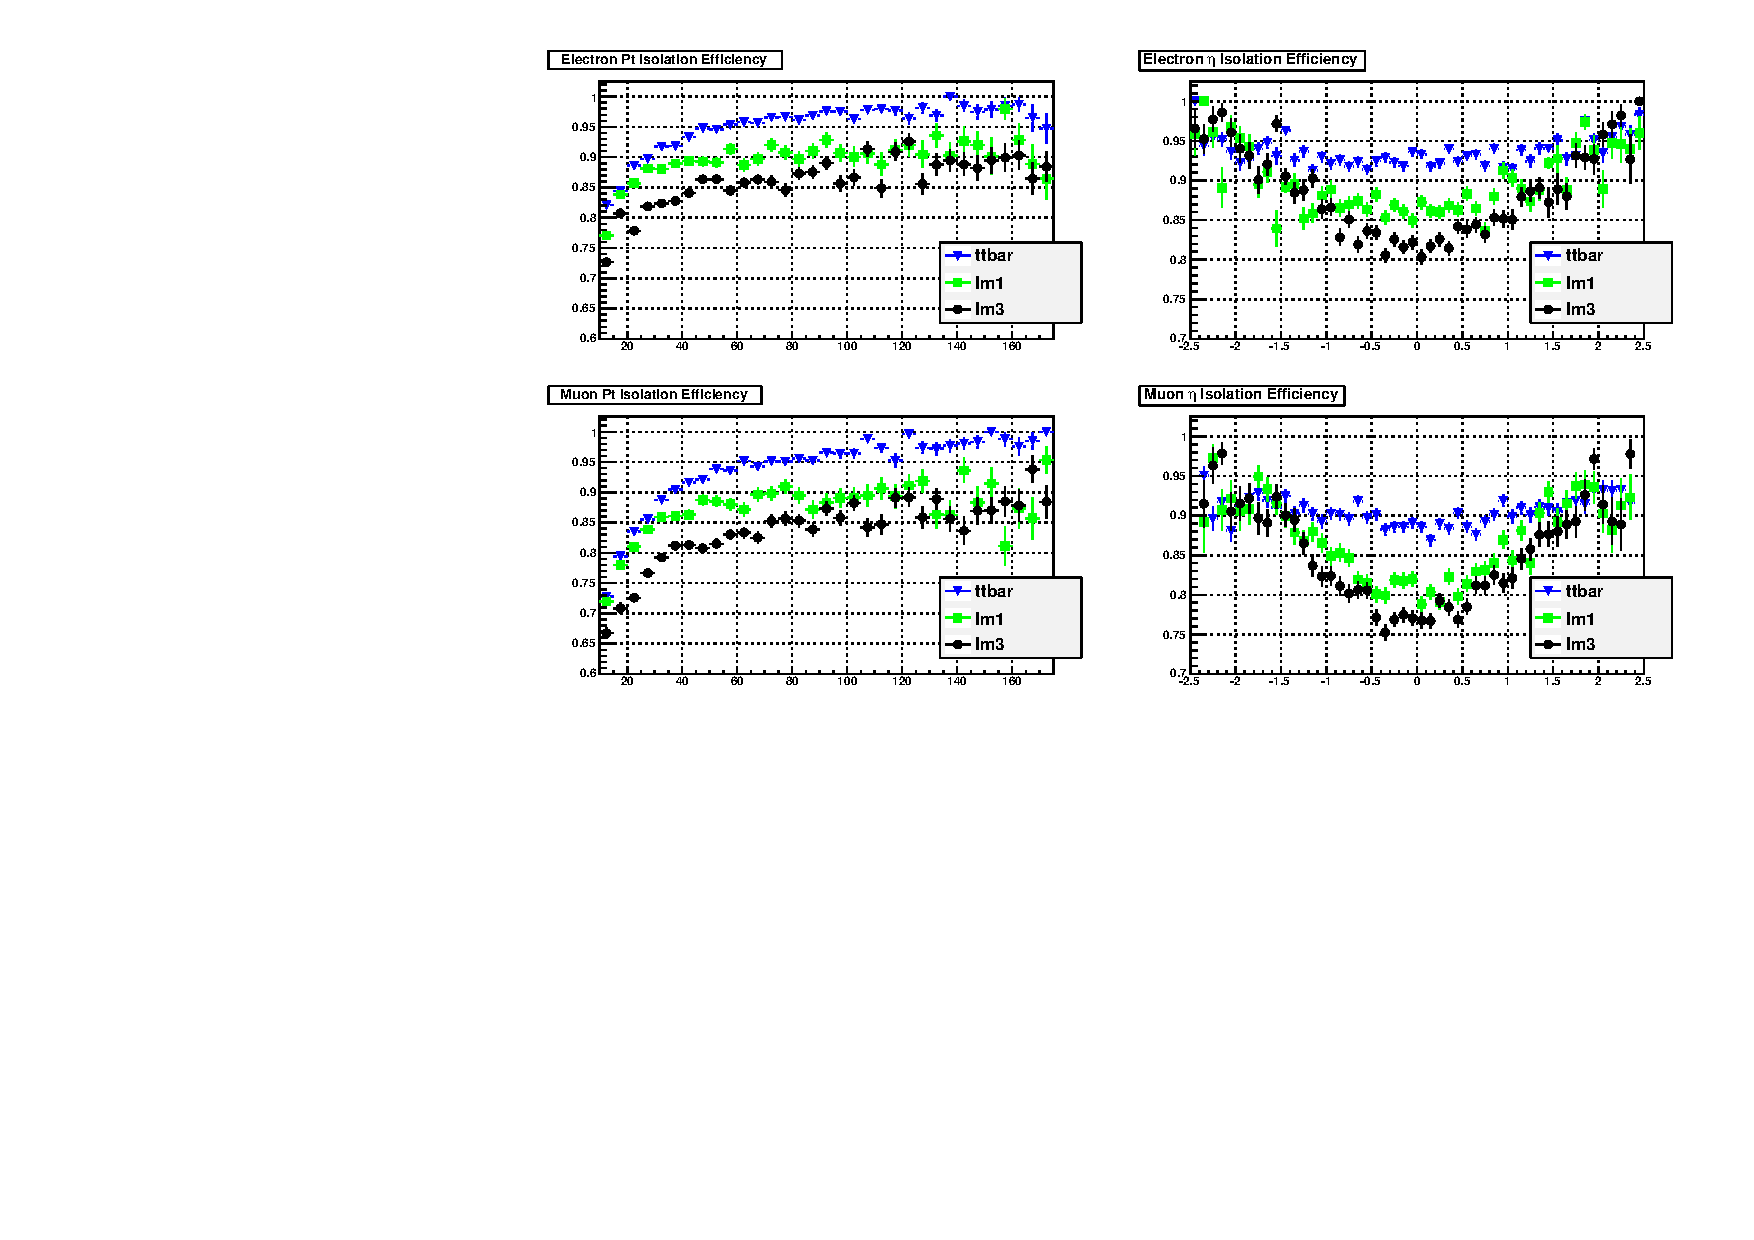
\includegraphics[width=\linewidth]{plots/tt_and_lm_isolationEfficiencies.pdf}
\caption{\label{fig:leptoniso} 
The lepton isolation efficiencies for \ttbar, LM1 and LM3 MC for electrons (top) and muons (bottom)
vs. \pt\ (left) and $\eta$ (right).
}
\end{center}
\end{figure}


%model-dependent limits
\clearpage
\section{Model-Dependent Limits}
\label{sec:models}

As an example of how the upper limit presented in Sec.~\ref{sec:upperlimit} can be
used to test if a specific model is excluded, in this section we consider the benchmark
SUSY processes LM4 and LM8, which contain
$Z$ bosons produced in the cascade decays of SUSY particles. 
We place upper limits on the quantity $\sigma \times BF \times A$,
assuming efficiencies and uncertainties from these processes, and compare them to 
the expected values of $\sigma \times BF \times A$.
Here $\sigma$ is the signal production cross section, $BF$ is the branching fraction
to the final state Z + jets + MET and $A$ is the signal acceptance.
%{\bf I am showing ttbar below, in addition to LM4 and LM8, but perhaps this should be removed...}

The signal event yield $N_{SIG}$ can be expressed as:

\begin{equation}
N_{SIG} = \sigma \times BF \times A \times \epsilon \times \mathcal{L},
\end{equation}

and we therefore have:

\begin{equation}
N_{SIG}/( \epsilon \times \mathcal{L}) = \sigma \times BF \times A.
\end{equation}

Here  $\epsilon$ is the signal efficiency and $\mathcal{L}$ is the integrated luminosity. 
Since we wish to place an upper limit on the quantity $\sigma \times BF \times A$, we must evaluate
the quantity $N_{SIG}/(\epsilon \times \mathcal{L})$.  Because of the efficiency
in the denominator, this upper limit cannot be calculated in an entirely model-independent
way; rather, it must be calculated with respect to a specific model. We therefore evaluate
the upper limit on $\sigma \times BF \times A$ with respect to $t\bar{t}$, LM4 and LM8.  
For each process, we must calculate both the efficiency and its uncertainty, as discussed
in the following subsections.



\subsection{Signal Efficiencies}
\label{sec:sigeff}

We evaluate the signal efficiencies using MC. To evaluate these efficiencies for our sample processes, 
we take as our denominator the number of generated events which pass the following selection at
the generator level:

\begin{itemize}
\item 2 electrons or muons with $p_T>20$~GeV and $|\eta|<2.5$,
\item Opposite-sign, same-flavor pair with $81 < M(ll) < 101$~GeV,
\item Count genjets with $p_T > 30$~GeV, $|\eta|<2.5$, $\Delta R > 0.4$ from any selected lepton as defined above,
\item At least 2 genjets.
\end{itemize}

For the loose (tight) signal region efficiency, we add to this the requirement genmet$>60$ (120)~GeV.
We take as our numerator the number of events passing the above generator-level selection which
also pass the signal region selection at reco-level. 
%{\bf Should I also consider events passing reco-selection which do NOT pass gen-level selection? For ttbar this
%\bf is a large effect, it is small for LM4 and LM8. }
For the loose (tight) signal region we find efficiencies of 43\% (42\%), 54\% (55\% )and 45\% (48\%) 
for $t\bar{t}$, LM4 and LM8, respectively.
This efficiency is dominated by the dilepton selection efficiency, which varies from $\sim0.6-0.7$ for the chosen 
processes. 

%The efficiency for selected dileptons to satisfy the dilepton mass requirement is $\sim0.9$;
%the efficiency to satisfy the requirements on the jet multiplicity is $\sim0.8-0.9$, for the MET$>60$~GeV requirement
%this efficiency is $\sim0.9-1$. 


%%%%%%%%%%%%%%%%%%%%%%%%%%%%%%%%%%%%%%%%%%%%%%%
%this section has been copied into systematics.tex


\subsection{Signal Efficiency Uncertainties}

Here we assess systematic uncertainties in the signal efficiencies for our sample processes, from
jet/MET, lepton identification, and luminosity uncertainties. 

\begin{itemize}
  
\item Jets and MET selection efficiency: we assess this uncertainty by varying the hadronic energy scale by $\pm 5\%$
  following the procedure used in the ttdilepton cross-section measurement.  For the loose (tight) signal regions 
  we find uncertainties of 9\% (23\%), 2\% (4\%), and 2\%(4\%) for  $t\bar{t}$, LM4 and LM8, respectively.
\item Lepton ID and isolation efficiencies: we perform a tag-and-probe technique
  on Z data and MC and find that the simulation agrees with data within about 2\% as shown in Table~\ref{tab:tagandprobe}.
  We apply a conservative 5\% uncertainty on the dilepton selection efficiency.
\item Trigger efficiency: the trigger efficiency is very close to 1 since there are 2 leptons with \pt $> 20$ GeV.
  We apply the simplified model of the trigger efficiency documented in~\cite{ref:GenericOS} and assess the uncertainty
  as the relative difference in the yields between assuming 100\% trigger efficiency vs. using the trigger model. This
  procedure gives differences of less than 1\% and the trigger efficiency uncertainty is therefore regarded as negligible.
\item Luminosity: we assess an uncertainty of 11\%.

\end{itemize}

\begin{table}[hbt]
\begin{center}
\caption{\label{tab:tagandprobe} Tag and probe results on $Z \to \ell \ell$
on data and MC.  We quote ID efficiency given isolation and 
the isolation efficiency given ID. }
\begin{tabular}{|l||c|c|}
\hline
                       & Data  T\&P        & MC T\&P               \\  
\hline
$\epsilon(id|iso)$ els & 0.918 $\pm$ 0.003 & 0.936 $\pm$ 0.0038    \\ 
$\epsilon(iso|id)$ els & 0.986 $\pm$ 0.001 & 0.987 $\pm$ 0.0018    \\
$\epsilon(id|iso)$ mus & 0.962 $\pm$ 0.002 & 0.964 $\pm$ 0.0027    \\
$\epsilon(iso|id)$ mus & 0.987 $\pm$ 0.001 & 0.984 $\pm$ 0.0018    \\
\hline

\end{tabular}
\end{center}
\end{table}

\subsection{Upper Limits on $\sigma \times BF \times A$}

Armed with the efficiencies and uncertainties calculated in the previous 2 sections, we proceed
to calculate upper limits on the quantity $\sigma \times BF \times A$. We calculate Bayesian 95\% CL upper
limits using the cl95cms software, assuming a log-normal model of nuissance parameter integration.
We also calculate the quantity $\sigma \times BF \times A$ for LM4 and LM8, for which we assume LO
cross-sections of 1.88~pb and 0.73~pb and calculate k-factors for each event, depending on the sub-process.
The quantity $BF \times A$ is taken to be the fraction of the total number of generated events which
pass the generator-level selection given in Sec.~\ref{sec:sigeff}. The results are summarized in
Table~\ref{tab:models}. These results show that the LM4 and LM8 benchmark points are beyond the
sensitivity of this search with the current integrated luminosity.

\begin{table}[hbt]
\begin{center}
\caption{\label{tab:models} Summary of efficiencies, efficiency uncertainties (quadrature sum
of jet/MET, dilepton and luminosity uncertainties), and upper limits on $\sigma \times BF \times A$ 
for the loose (MET$>60$~GeV) and tight (MET$>120$~GeV) signal regions. We also show the quantity
$\sigma \times BF \times A$ for LM4 and LM8.}
\begin{tabular}{l|ccc}

\hline
                                         & $t\bar{t}$    & LM4     & LM8       \\
\hline
{\bf Loose signal region}                &               &         &           \\
Efficiency                               &       0.43    & 0.54    & 0.45      \\
Efficiency Uncertainty                   &       0.15    & 0.12    & 0.12      \\
UL($\sigma \times BF \times A$) (pb)     &       0.56    & 0.44    & 0.53      \\
$\sigma \times BF \times A$ (pb)         &               & 0.045   & 0.025     \\

\hline
{\bf Tight signal region}                &               &         &           \\
Efficiency                               &       0.42    &  0.55   & 0.48      \\
Efficiency Uncertainty                   &       0.26    &  0.13   & 0.13      \\
UL($\sigma \times BF \times A$) (pb)     &       0.23    &  0.17   & 0.19      \\
$\sigma \times BF \times A$ (pb)         &               &  0.035  & 0.018     \\
 
\hline

\end{tabular}
\end{center}
\end{table}






%Double_t CL95(Double_t ilum, Double_t slum, Double_t eff, Double_t seff, 
%              Double_t bck, Double_t sbck, Int_t n, Bool_t gauss = kFALSE, Int_t nuisanceModel = 0)

%---------
%ttbar
%---------

%root [5] CL95( 34 , 0. , 0.43 , 0.15*0.43 , 6.04 , 0.96 , 7 , false , 1 )    
%Poisson 95% CL limit with Lognormal nuisance parameter integration will be used
%Likelihood function is evaluated over [0,2] 
%likelihood normalization: 0.0498808
%Info in <TCanvas::Print>: eps file Likelihood.eps has been created
%Upper 95% C.L. limit on signal = 0.561523 pb
%(Double_t)5.61523437500000000e-01

%---------
%LM4
%---------

%root [6] CL95( 34 , 0. , 0.54 , 0.12*0.54 , 6.04 , 0.96 , 7 , false , 1 )    
%Poisson 95% CL limit with Lognormal nuisance parameter integration will be used
%Likelihood function is evaluated over [0,2] 
%likelihood normalization: 0.0395872
%Info in <TCanvas::Print>: eps file Likelihood.eps has been created
%Upper 95% C.L. limit on signal = 0.44043 pb
%(Double_t)4.40429687500000000e-01

%---------
%LM8
%---------

%root [7] CL95( 34 , 0. , 0.45 , 0.12*0.45 , 6.04 , 0.96 , 7 , false , 1 )
%Poisson 95% CL limit with Lognormal nuisance parameter integration will be used
%Likelihood function is evaluated over [0,2] 
%likelihood normalization: 0.0475047
%Info in <TCanvas::Print>: eps file Likelihood.eps has been created
%Upper 95% C.L. limit on signal = 0.52832 pb
%(Double_t)5.28320312500000000e-01

%\clearpage
%\section{Conclusion}
%\label{sec:conclusion}

This note presents a search for the production of stop quark pairs in events with a 
single isolated lepton, several jets, missing transverse energy, and
large transverse mass. The dataset used corresponds to an integrated
luminosity of \lumi\ at center-of-mass energy of 8 TeV. Seven signal
regions are defined, based on \met\ and \mt\ requirements. Agreement is
observed between the data and the predicted backgrounds for all signal
regions. The results are interpreted in the context of simplified SUSY
models where the stops decay to top-neutralino or b-chargino and are
used to place constraints on the stop mass.


\clearpage
\begin{thebibliography}{10}
%  \bibitem {NOTE000} {\bf CMS Note 2005/000},
%    X.Somebody et al.,
%    {\em "CMS Note Template"}.

\bibitem{ref:Ztemplates} ADD REF TO MET TEMPLATES NOTE, WHEN AVAILABLE

\bibitem{ref:osnote} CMS AN-2010/370

\bibitem{ref:ospaper} arXiv:1103.1348v1 [hep-ex], ``Search for Physics Beyond the Standard Model in Opposite-Sign Dilepton Events at $\sqrt{s} = 7$~TeV.''

\bibitem{ref:top} Phys.Lett.B695:424-443,2011 

\bibitem{ref:vbtf} https://twiki.cern.ch/twiki/bin/viewauth/CMS/SimpleCutBasedEleID

\bibitem{ref:conv} D.~Barge {\em at al.}, AN-CMS2009/159.

\bibitem{ref:xsec} https://twiki.cern.ch/twiki/bin/view/CMS/ProductionReProcessingSpring10 
% {\color{red} Is this the right reference?}


\bibitem{ref:victory}V.~Pavlunin, Phys. Rev. {\bf D81}, 035005 (2010).

\bibitem{ref:ourvictory}  D.~Barge {\em at al.}, AN-CMS2009/130.

\bibitem{ref:dy} W.~Andrews {\em et al.}, AN-CMS2009/023.

\bibitem{ref:FR} D.~Barge {\em at al.}, AN-CMS2010/257.

\bibitem{ref:evans}W.~Andrews {\em et al.}, AN-CMS2010/274.

\bibitem{ref:bayes.f} J.~Conway, {\tt http://www-cdf.fnal.gov/physics/statistics/code/bayes.f}.

\bibitem{ref:cl95cms} G.~Landsberg, {\tt https://twiki.cern.ch/twiki/pub/CMS/EXOTICA/cl95cms.c}

\bibitem{ref:scan} {\tt https://hypernews.cern.ch/HyperNews/CMS/get/susy/617/2/1.html}

\bibitem{ref:sanjay} {\tt https://twiki.cern.ch/twiki/bin/view/CMS/SUSY38XSUSYScan}

\bibitem{ref:pdf} arXiv:hep-ph/0605240v2

\bibitem{ref:smooth} {\tt CleanExclusion.cc} available at
{\tt https://twiki.cern.ch/twiki/bin/viewauth/CMS/SUSYLimitTools}

\bibitem{ref:cousins} R.~Cousins, {\tt http://www.physics.ucla.edu/\~cousins/stats/cousins\_lognormal\_prior.pdf}

\bibitem{ref:harper} S.~Harper, private communication (relayed to us by M.~Chiorboli.).

\bibitem{ref:MT2} A. Barr {\em at al.}, J.Phys.G29:2343-2363,2003;
Cheng, H.C., Han, arXiv:hep-ph/0810.5178v2.\\
{\tt http://indico.cern.ch/contributionDisplay.py?contribId=3\&confId=66410}

\bibitem{ref:MT2J} {\tt http://indico.cern.ch/contributionDisplay.py?contribId=5\&confId=93837}

\bibitem{ref:brown} M.~Narain {\em et al.}, CMS AN-2010/259; we thank the 
Brown group for providing their code to us.


    
\end{thebibliography}


\clearpage
\appendix
\section{Triggers}

When listing triggers in this section, the version number is omitted for simplicity.

\subsection{Dilepton Triggers}
\label{app:trigsel}

The triggers used for selecting dilepton events are:

\begin{itemize}
\item double-muon triggers
  \begin{itemize}
  \item \verb=HLT_DoubleMu7_v=
  \item \verb=HLT_Mu13_Mu7_v=
  \end{itemize}
\item double-electron triggers
  \begin{itemize}
  \item \verb=HLT_Ele17_CaloIdL_CaloIsoVL_Ele8_CaloIdL_CaloIsoVL_v=
  \item \verb=HLT_Ele17_CaloIdT_TrkIdVL_CaloIsoVL_TrkIsoVL_Ele8_CaloIdT_TrkIdVL_CaloIsoVL_TrkIsoVL_v=
  \end{itemize}
\item e-$\mu$ cross triggers
  \begin{itemize}
  \item \verb=HLT_Mu17_Ele8_CaloIdL_v=
  \item \verb=HLT_Mu8_Ele17_CaloIdL_v=
  \end{itemize}
\end{itemize}


\subsection{Photon Triggers}
\label{app:photrig}

The photon triggers used are:

\begin{itemize}
\item \verb=HLT_Photon20_CaloIdVL_IsoL_v= (\Z \pt $<$ 33~GeV)
\item \verb=HLT_Photon30_CaloIdVL_IsoL_v= (33 GeV $<$ \Z \pt $<$ 55~GeV)
\item \verb=HLT_Photon50_CaloIdVL_IsoL_v= (55 GeV $<$ \Z \pt $<$ 81~GeV)
\item \verb=HLT_Photon75_CaloIdVL_IsoL_v= (\Z \pt $>$ 81~GeV)
\end{itemize}

The HLT requirements on the above triggers are \cite{ref:eghlt}:

\begin{itemize}
\item CaloIdVL: \\
  H/E $<$ 0.15 (0.1), $\sigma_{i\eta i\eta} <$ 0.024 (0.04) in barrel (endcap)
\item IsoL: \\
  Ecal ET $<$ 5.5 + 0.012*ET, %\\
  Hcal ET $<$ 3.5 + 0.005*ET, %\\
  Trk PT $<$ 3.5 + 0.002*ET 
\end{itemize}


\subsection{Jet Triggers}
\label{app:jettrig}

The single jet triggers used to select the QCD sample from which the QCD MET templates are derived are listed below along with the thresholds applied to the lead jet pt for each trigger:

% {0, 70, 90, 130, 180, 220, 270, 340, 400};

\begin{itemize}
\item \verb=HLT_Jet30_v=  (\pt $>$ 0 )
\item \verb=HLT_Jet60_v=  (\pt $>$ 70 )
\item \verb=HLT_Jet80_v=  (\pt $>$ 90 )
\item \verb=HLT_Jet110_v= (\pt $>$ 130 )
%we don't use these bc threshold is too high for our sjp binning
%\item \verb=HLT_Jet150_v= (\pt $>$ 180 )
%\item \verb=HLT_Jet190_v= (\pt $>$ 220 )
%\item \verb=HLT_Jet240_v= (\pt $>$ 270 )
%\item \verb=HLT_Jet300_v= (\pt $>$ 340 )
%\item \verb=HLT_Jet370_v= (\pt $>$ 400 )
\end{itemize}


%%%%%%%%%%%%%%%%%%%%%%%%%%%%%%%%%%%%%%
%2010 triggers

%\begin{itemize}
%\item single-muon triggers
%  \begin{itemize}
%  \item \verb=HLT_Mu5=
%  \item \verb=HLT_Mu7=        
%  \item \verb=HLT_Mu9=         
%  \item \verb=HLT_Mu11=       
%  \item \verb=HLT_Mu13_v1=     
%  \item \verb=HLT_Mu15_v1=     
%  \item \verb=HLT_Mu17_v1=     
%  \item \verb=HLT_Mu19_v1=     
%  \end{itemize}
%\item double-muon triggers
%  \begin{itemize}
%  \item \verb=HLT_DoubleMu3=
%  \item \verb=HLT_DoubleMu3_v2=
%  \item \verb=HLT_DoubleMu5_v1=
%  \end{itemize}
%\item single-electron triggers
%  \begin{itemize}
%  \item \verb=HLT_Ele10_SW_EleId_L1R=
%  \item \verb=HLT_Ele10_LW_EleId_L1R=
%  \item \verb=HLT_Ele10_LW_L1R=
%  \item \verb=HLT_Ele10_SW_L1R=
%  \item \verb=HLT_Ele15_SW_CaloEleId_L1R=
%  \item \verb=HLT_Ele15_SW_EleId_L1R=
%  \item \verb=HLT_Ele15_SW_L1R=
%  \item \verb=HLT_Ele15_LW_L1R=
%  \item \verb=HLT_Ele17_SW_TightEleId_L1R=
%  \item \verb=HLT_Ele17_SW_TighterEleId_L1R_v1=
%  \item \verb=HLT_Ele17_SW_CaloEleId_L1R=
%  \item \verb=HLT_Ele17_SW_EleId_L1R=
%  \item \verb=HLT_Ele17_SW_LooseEleId_L1R=
%  \item \verb=HLT_Ele17_SW_TighterEleIdIsol_L1R_v2=
%  \item \verb=HLT_Ele20_SW_L1R=
%  \item \verb=HLT_Ele22_SW_TighterEleId_L1R_v2=
%  \item \verb=HLT_Ele32_SW_TightCaloEleIdTrack_L1R_v1=
%  \item \verb=HLT_Ele32_SW_TighterEleId_L1R_v2=
%  \item \verb=HLT_Ele27_SW_TightCaloEleIdTrack_L1R_v1=
%  \item \verb=HLT_Ele22_SW_TighterCaloIdIsol_L1R_v2=
%  \item \verb=HLT_Ele22_SW_TighterEleId_L1R_v3=
%  \item \verb=HLT_Ele22_SW_TighterCaloIdIsol_L1R_v2=
%  \end{itemize}
%\item double-electron triggers
%  \begin{itemize}
%  \item \verb=HLT_DoubleEle15_SW_L1R_v1=                 
%  \item \verb=HLT_DoubleEle17_SW_L1R_v1=   
%  \item \verb=HLT_Ele17_SW_TightCaloEleId_Ele8HE_L1R_v1=
%  \item \verb=HLT_Ele17_SW_TightCaloEleId_SC8HE_L1R_v1=
%  \item \verb=HLT_DoubleEle10_SW_L1R=
%  \item \verb=HLT_DoubleEle5_SW_L1R=
%  \end{itemize}
%\item e-$\mu$ cross triggers
%  \begin{itemize}
%  \item \verb=HLT_Mu5_Ele5_v1=
%  \item \verb=HLT_Mu5_Ele9_v1=
%  \item \verb=HLT_Mu11_Ele8_v1=
%  \item \verb=HLT_Mu8_Ele8_v1=
%  \item \verb=HLT_Mu5_Ele13_v2=
%  \item \verb=HLT_Mu5_Ele17_v1=
%  \end{itemize}
%\end{itemize}

\clearpage
\section{Kinematics of \emu ~Events}

We show here dilepton mass (figure \ref{fig:emudilmass}) and MET (figure \ref{fig:emudilmet}) distributions for opposite flavor (\emu) events.

\begin{figure}[hbt]
  \begin{center}
	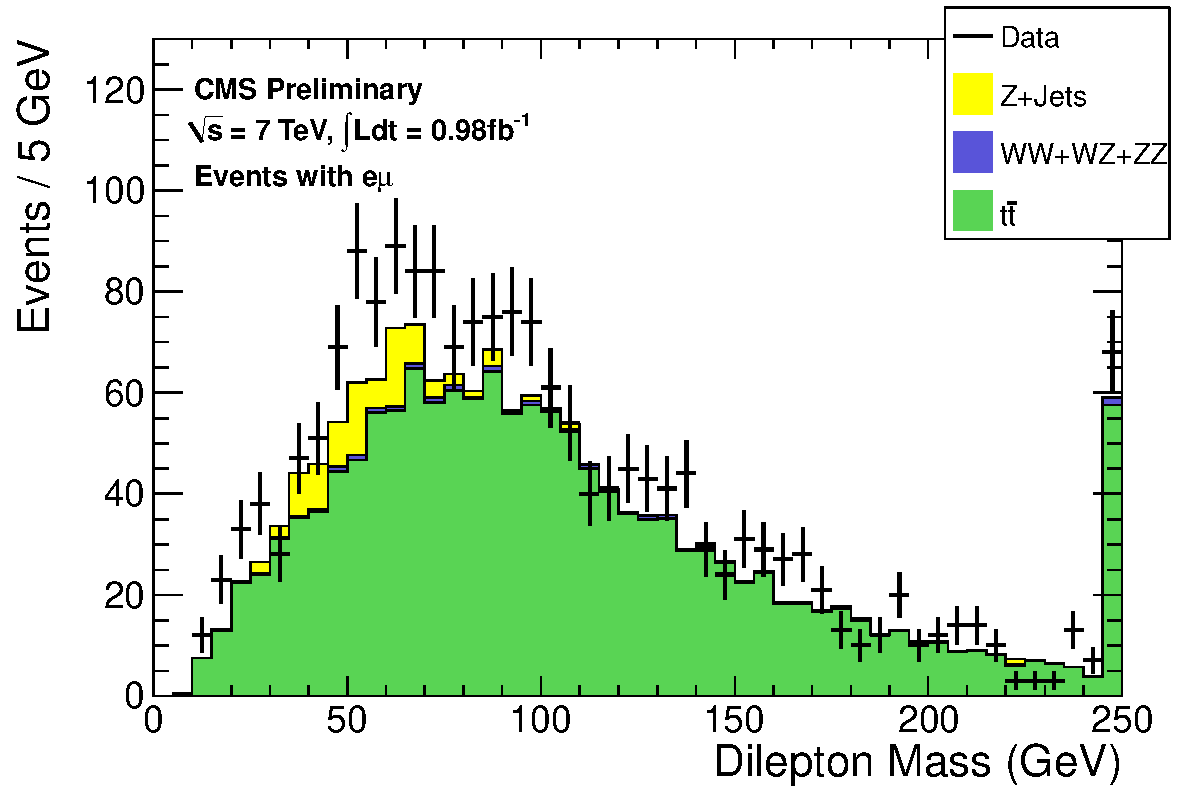
\includegraphics[width=0.48\linewidth]{plots/hdilmass_em_allj.pdf}
	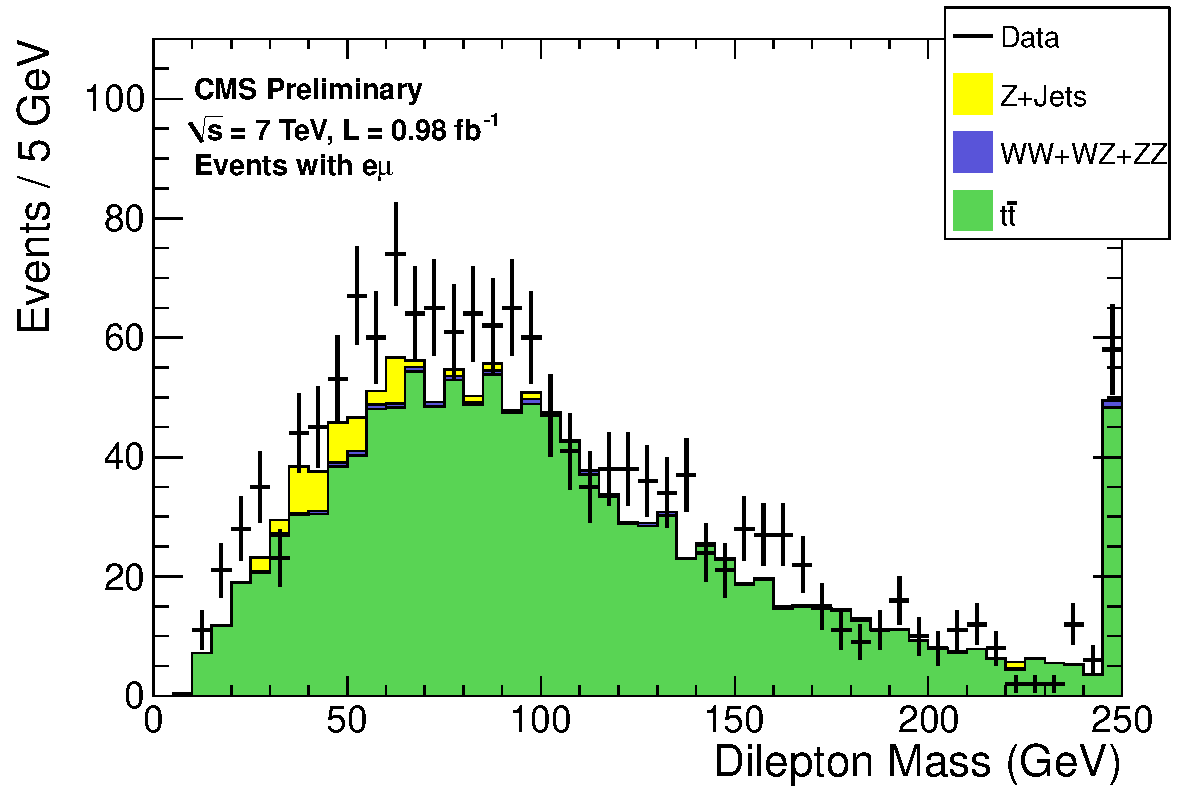
\includegraphics[width=0.48\linewidth]{plots/hdilmass_pfmet30_em_allj.pdf}
	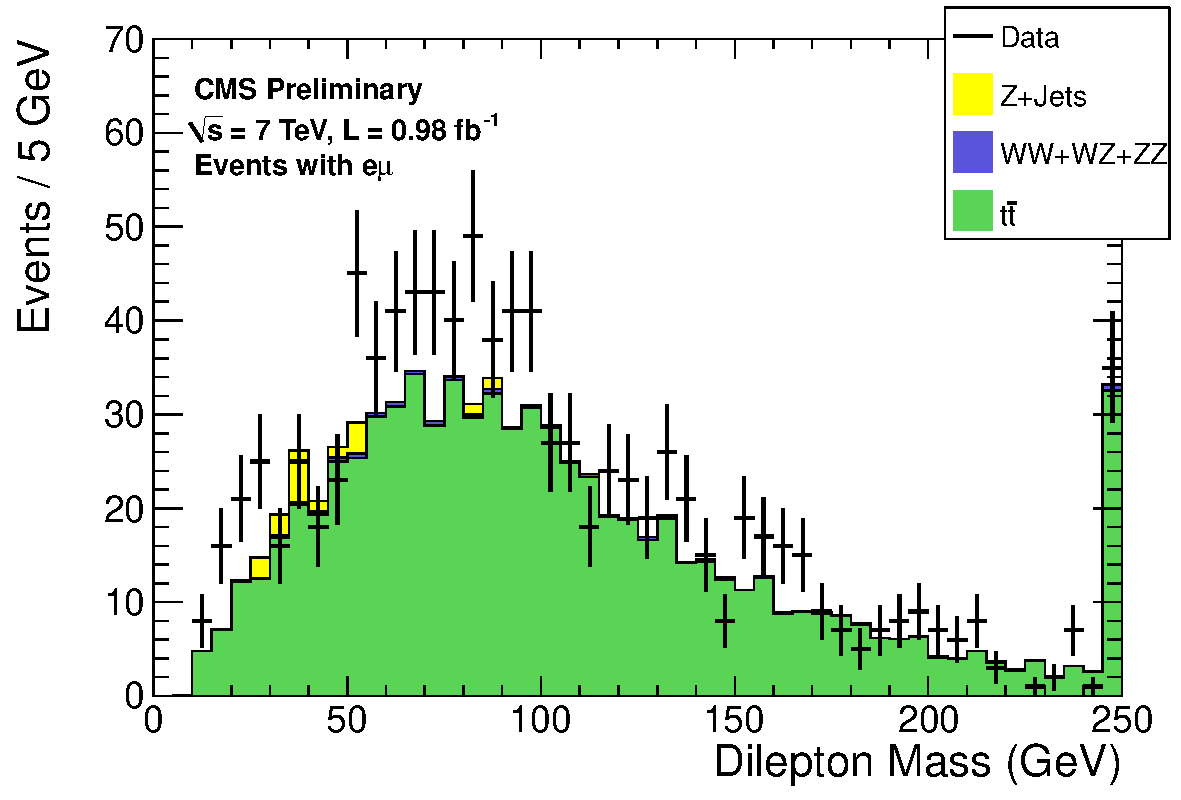
\includegraphics[width=0.48\linewidth]{plots/hdilmass_pfmet60_em_allj.pdf}
	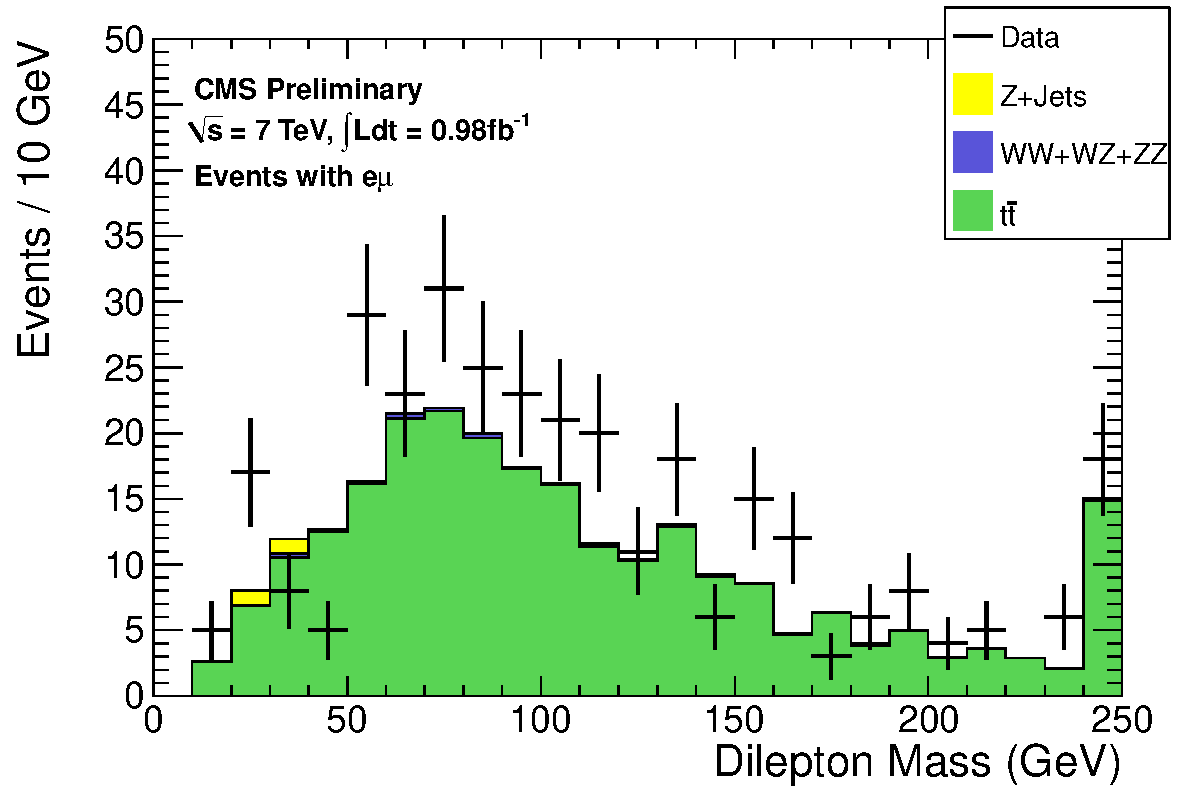
\includegraphics[width=0.48\linewidth]{plots/hdilmass_pfmet100_em_allj.pdf}
	\caption{
	  \label{fig:emudilmass}\protect 
	  Dilepton mass distribution for opposite flavor events ($\ge$ 2 jets)
	  with no MET cut (top left),
	  MET $>$ 30 (top right),
	  MET $>$ 60 (bottom left), and
	  MET $>$ 100 (top right).
	}
  \end{center}
\end{figure}

\begin{figure}[hbt]
  \begin{center}
	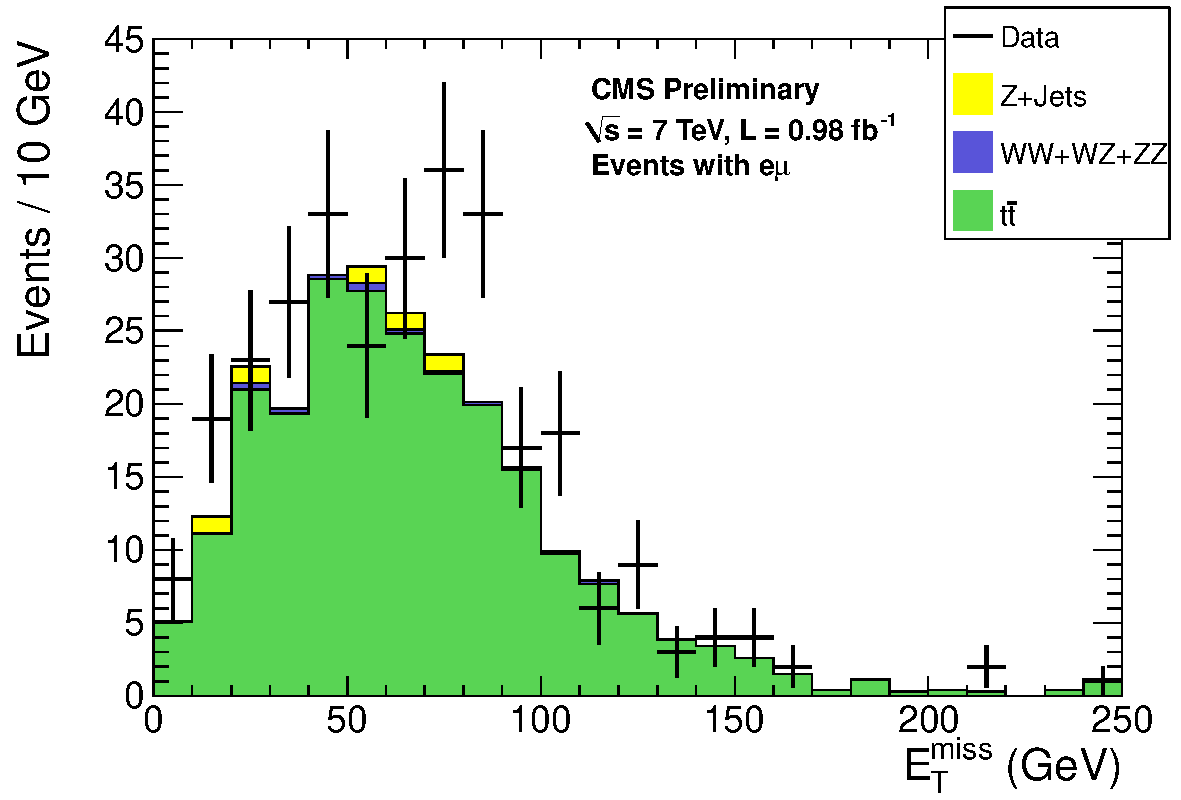
\includegraphics[width=0.8\linewidth]{plots/hdilmet_em_allj.pdf}
	\caption{
	  \label{fig:emudilmet}\protect 
	  MET distribution for opposite flavor events ($\ge$ 2 jets)
	  with no a Z mass (81 to 101 GeV) requirement.
	}
  \end{center}
\end{figure}

\clearpage

\section{Details of Events in Loose Signal Region}
\label{sec:sigevts}

In this appendix we show details of events in the loose signal region (MET $>$ \signalmetl~GeV) 
for \lumi ~in tables \ref{sig60eventsee} (for \ee ~events) and \ref{sig60eventsmm} (for \mm ~events).

%2011 event table

\begin{table}[htb]
  \begin{center}
	\caption{
	  \label{sig60eventsee} 
	  Details of \ee ~data events for the loose signal region 
	  MET $>$ \signalmetl GeV for \lumi. The SimpleSecondaryVertexTagger high efficiency medium 
	  working point is used for b-tagging.}

  %IS THIS STILL TRUE???
  %, for which the efficiency is $\sim40$\% and the mistag rate is $\sim1$\%.}
  \begin{tabular}{rrrrrrrrrrr}

	\hline
Run & Lumi & Event & Lep & Njet & N B Tag & pfMET & tcMET & Dilep & Sum & Z \pt\\
 &  Section &  & Type &  &  &  &  & Mass  & jet \pt & \\
\hline

161312 & 963 &  366557890 &    $e$ & 4 & 2 & 117.1 & 117.9 &  89.0 & 219.6 &  18.1\\
163069 & 432 &  236566401 &    $e$ & 2 & 1 & 107.4 &  92.3 &  83.6 & 215.4 &  90.9\\
163758 &  86 &   64208683 &    $e$ & 2 & 0 & 119.5 & 114.1 &  82.6 & 113.3 &  58.6\\
163758 &  63 &   46610542 &    $e$ & 4 & 0 & 124.1 &  41.4 &  91.1 & 301.0 & 261.9\\
163332 & 615 &  415350358 &    $e$ & 4 & 0 & 115.6 & 108.6 & 100.1 & 341.3 & 108.3\\
163332 & 730 &  489406176 &    $e$ & 2 & 0 & 100.4 &  88.4 &  92.6 & 114.8 &  52.8\\
163817 & 680 &  633297354 &    $e$ & 4 & 0 & 165.0 & 155.0 &  89.7 & 439.6 &  26.0\\
165467 &  42 &   25220649 &    $e$ & 3 & 1 & 107.7 & 100.3 & 100.2 & 208.9 &  34.0\\
165567 & 145 &  162118370 &    $e$ & 3 & 0 & 108.6 & 105.7 &  82.9 & 1613.0 &  78.6\\
165567 & 134 &  146666450 &    $e$ & 3 & 1 & 162.8 & 157.2 &  86.3 & 285.5 &  35.1\\
165570 &  90 &  114117797 &    $e$ & 3 & 0 & 133.1 & 109.3 &  94.8 & 311.3 & 106.2\\
165617 & 121 &  164071172 &    $e$ & 2 & 1 & 133.9 & 137.0 &  83.4 & 197.2 &  24.4\\
165993 & 886 &  985111484 &    $e$ & 2 & 0 & 247.4 & 258.1 &  90.7 & 358.2 &  35.0\\
166049 &  96 &  104394022 &    $e$ & 2 & 0 & 111.3 & 104.6 &  96.7 & 126.1 &  64.7\\
166380 & 931 & 1022715220 &    $e$ & 2 & 1 & 140.2 & 146.9 &  85.4 & 230.7 &  16.4\\
166512 & 1337 & 1503207759 &    $e$ & 4 & 2 & 127.1 & 118.8 &  85.4 & 292.1 &  31.6\\
166554 & 379 &  452347639 &    $e$ & 2 & 1 & 122.1 & 115.5 &  94.6 & 248.7 &  11.0\\
166699 & 262 &  274276792 &    $e$ & 2 & 0 & 108.1 &  92.4 &  90.1 & 129.8 &  37.0\\
166699 & 868 &  913050834 &    $e$ & 2 & 0 & 102.5 & 129.9 &  86.1 & 144.2 & 177.7\\
166782 & 144 &  161600405 &    $e$ & 3 & 1 & 115.4 & 146.3 &  95.0 & 288.3 &  63.3\\
166787 &  48 &   42718322 &    $e$ & 2 & 1 & 154.3 & 151.8 &  98.2 & 140.3 &  57.4\\
166864 & 114 &  119336561 &    $e$ & 2 & 1 & 130.8 & 111.7 &  82.4 & 120.4 &  44.4\\
166889 & 143 &  168814966 &    $e$ & 2 & 0 & 119.7 & 121.1 &  92.9 & 257.5 & 154.4\\
167102 & 109 &  113554882 &    $e$ & 3 & 1 & 163.9 & 174.7 &  90.3 & 429.1 & 205.8\\
167675 & 261 &  285970917 &    $e$ & 3 & 0 & 101.6 &  95.7 &  88.6 & 214.3 &  39.1\\

	\hline
  \end{tabular}
\end{center}
\end{table}



\begin{table}[htb]
  \begin{center}
	\caption{
	  \label{sig60eventsmm} 
	  Details of \mm ~data events for the loose signal region 
	  MET $>$ \signalmetl GeV for \lumi. The SimpleSecondaryVertexTagger high efficiency medium 
	  working point is used for b-tagging.}

  %IS THIS STILL TRUE???
  %, for which the efficiency is $\sim40$\% and the mistag rate is $\sim1$\%.}
  \begin{tabular}{rrrrrrrrrrr}

	\hline
Run & Lumi & Event & Lep & Njet & N B Tag & pfMET & tcMET & Dilep & Sum & Z \pt\\
 &  Section &  & Type &  &  &  &  & Mass  & jet \pt & \\
\hline

163659 & 320 &  243264615 &  $\mu$ & 2 & 0 & 150.0 & 130.2 &  86.1 & 193.6 &  71.1\\
163663 & 181 &  126212285 &  $\mu$ & 3 & 1 & 102.3 &  79.9 &  85.4 & 212.1 &  49.8\\
163584 &  54 &   39429230 &  $\mu$ & 3 & 0 & 209.6 & 217.4 &  92.5 & 348.4 &  29.2\\
160873 & 115 &   30074254 &  $\mu$ & 2 & 1 & 102.8 &  87.8 &  89.1 &  90.7 &  78.5\\
163255 & 673 &  435619707 &  $\mu$ & 2 & 2 & 169.4 & 160.6 &  96.0 & 140.4 & 108.0\\
163759 &  80 &   52493009 &  $\mu$ & 2 & 0 & 239.3 & 229.0 &  87.5 & 200.8 & 109.4\\
163233 &   8 &    3963812 &  $\mu$ & 2 & 0 & 106.2 & 103.3 &  82.9 & 123.8 &  58.0\\
165415 & 461 &  542228927 &  $\mu$ & 2 & 0 & 121.5 & 117.8 &  87.3 & 140.2 &  94.2\\
165467 & 373 &  474997628 &  $\mu$ & 3 & 0 & 157.2 & 142.4 &  90.7 & 246.4 &  77.1\\
165514 & 266 &  349995997 &  $\mu$ & 2 & 1 & 185.3 & 188.2 &  87.4 & 156.6 & 141.5\\
165570 & 228 &  305480522 &  $\mu$ & 4 & 0 & 175.6 & 197.0 &  98.3 & 477.1 &   6.4\\
165633 & 360 &  469114910 &  $\mu$ & 3 & 1 & 139.5 & 144.2 &  91.4 & 270.4 &  23.9\\
165993 & 432 &  490867631 &  $\mu$ & 1 & 0 & 132.1 & 137.5 &  92.1 & 172.3 & 145.4\\
166462 & 131 &  113312244 &  $\mu$ & 2 & 1 & 100.1 &  89.4 &  92.1 & 190.0 &  82.8\\
166512 & 534 &  647541425 &  $\mu$ & 2 & 2 & 106.7 & 105.6 &  85.9 & 155.7 &  14.1\\
166512 & 1257 & 1427678466 &  $\mu$ & 3 & 1 & 162.6 & 138.1 &  99.7 & 410.8 &  77.8\\
166512 & 289 &  347706349 &  $\mu$ & 2 & 1 & 119.5 & 127.3 &  86.1 & 165.9 & 121.7\\
166514 & 377 &  322005853 &  $\mu$ & 4 & 1 & 148.3 & 149.7 &  90.7 & 285.8 &  18.0\\
166514 & 203 &  174838511 &  $\mu$ & 2 & 2 & 166.7 & 152.6 &  86.2 & 209.2 &  59.4\\
166554 & 264 &  313635378 &  $\mu$ & 2 & 1 & 106.6 & 100.4 &  86.8 & 216.9 &  48.8\\
166699 & 842 &  888276647 &  $\mu$ & 3 & 0 & 103.9 & 108.6 & 100.7 & 403.6 &  48.1\\
166763 & 450 &  504667153 &  $\mu$ & 2 & 1 & 137.7 & 113.6 &  88.8 & 140.7 &  51.7\\
166781 & 122 &  134735813 &  $\mu$ & 2 & 1 & 101.9 & 104.6 &  81.2 & 128.0 &  91.4\\
166781 &  44 &   38030398 &  $\mu$ & 2 & 2 & 125.7 & 117.8 &  83.8 & 127.8 &  34.9\\
166841 & 643 &  689632265 &  $\mu$ & 2 & 1 & 122.8 & 124.6 &  81.9 & 239.2 &  87.2\\
166889 &  96 &  112612008 &  $\mu$ & 3 & 2 & 104.8 & 107.1 &  94.4 & 197.9 &  68.3\\
166890 & 210 &  234487675 &  $\mu$ & 1 & 0 & 145.0 & 129.4 &  93.6 & 119.2 &  40.3\\
166960 &  15 &   12353542 &  $\mu$ & 4 & 0 & 249.0 & 238.8 &  90.7 & 225.3 & 158.2\\
167103 &  57 &   52790466 &  $\mu$ & 3 & 0 & 184.0 & 182.5 &  82.6 & 274.2 &  86.3\\
167281 & 455 &  558976091 &  $\mu$ & 5 & 1 & 117.1 & 155.7 & 100.4 & 657.1 & 139.6\\
167284 & 791 &  676680323 &  $\mu$ & 3 & 1 & 134.6 & 142.2 &  81.9 & 226.9 &  18.2\\
167284 & 599 &  520467665 &  $\mu$ & 2 & 1 & 108.7 &  92.5 &  86.0 & 152.4 &  88.8\\
167674 & 168 &  206898581 &  $\mu$ & 1 & 0 & 137.4 & 136.4 &  90.0 & 126.7 &  27.7\\
167676 & 408 &  364168743 &  $\mu$ & 2 & 0 & 167.3 & 159.6 &  89.2 & 105.4 &  60.8\\
167676 & 236 &  215196501 &  $\mu$ & 3 & 1 & 117.7 & 117.3 &  96.6 & 159.6 &  75.7\\

	\hline
  \end{tabular}
\end{center}
\end{table}




\begin{comment}
% 204/pb

161312 & 963 &  366557890 &    $e$ & 4 & 2 & 117.1 & 117.9 &  89.0 & 218.9 &  18.1\\
163069 & 432 &  236566401 &    $e$ & 2 & 1 & 107.4 &  92.3 &  83.6 & 213.9 &  90.9\\
163758 &  86 &   64208683 &    $e$ & 2 & 0 & 119.5 & 114.1 &  82.6 & 114.0 &  58.6\\
163758 &  63 &   46610542 &    $e$ & 4 & 0 & 124.1 &  41.4 &  91.1 & 300.1 & 261.9\\
163332 & 615 &  415350358 &    $e$ & 4 & 0 & 115.6 & 108.6 & 100.1 & 316.7 & 108.3\\
163332 & 730 &  489406176 &    $e$ & 2 & 0 & 100.4 &  88.4 &  92.6 &  98.6 &  52.8\\
163817 & 680 &  633297354 &    $e$ & 4 & 0 & 165.0 & 155.0 &  89.7 & 437.8 &  26.0\\
163659 & 320 &  243264615 &  $\mu$ & 2 & 0 & 150.0 & 130.2 &  86.1 & 192.7 &  71.1\\
163663 & 181 &  126212285 &  $\mu$ & 3 & 1 & 102.3 &  79.9 &  85.4 & 210.5 &  49.8\\
163584 &  54 &   39429230 &  $\mu$ & 3 & 0 & 209.6 & 217.4 &  92.5 & 349.6 &  29.2\\
160873 & 115 &   30074254 &  $\mu$ & 2 & 1 & 102.8 &  87.8 &  89.1 &  89.9 &  78.5\\
163255 & 673 &  435619707 &  $\mu$ & 2 & 2 & 169.4 & 160.6 &  96.0 & 140.4 & 108.0\\
163759 &  80 &   52493009 &  $\mu$ & 2 & 0 & 239.3 & 229.0 &  87.5 & 198.7 & 109.4\\
163233 &   8 &    3963812 &  $\mu$ & 2 & 0 & 106.2 & 103.3 &  82.9 & 123.0 &  58.0\\

\end{comment}

\clearpage
\clearpage
\section{MET Templates from Photon Sample}
\label{sec:appendix_templates}

In this appendix we display our templates derived from the photon sample 
using the HLTPhoton20 (Fig.~\ref{fig:template20}), HLTPhoton30 (Fig.~\ref{fig:template30}),
HLTPhoton50 (Fig.~\ref{fig:template50}) and HLTPhoton70 (Fig.~\ref{fig:template70}) triggers.


\begin{figure}[hbt]
  \begin{center}
    \resizebox{0.7\linewidth}{!}{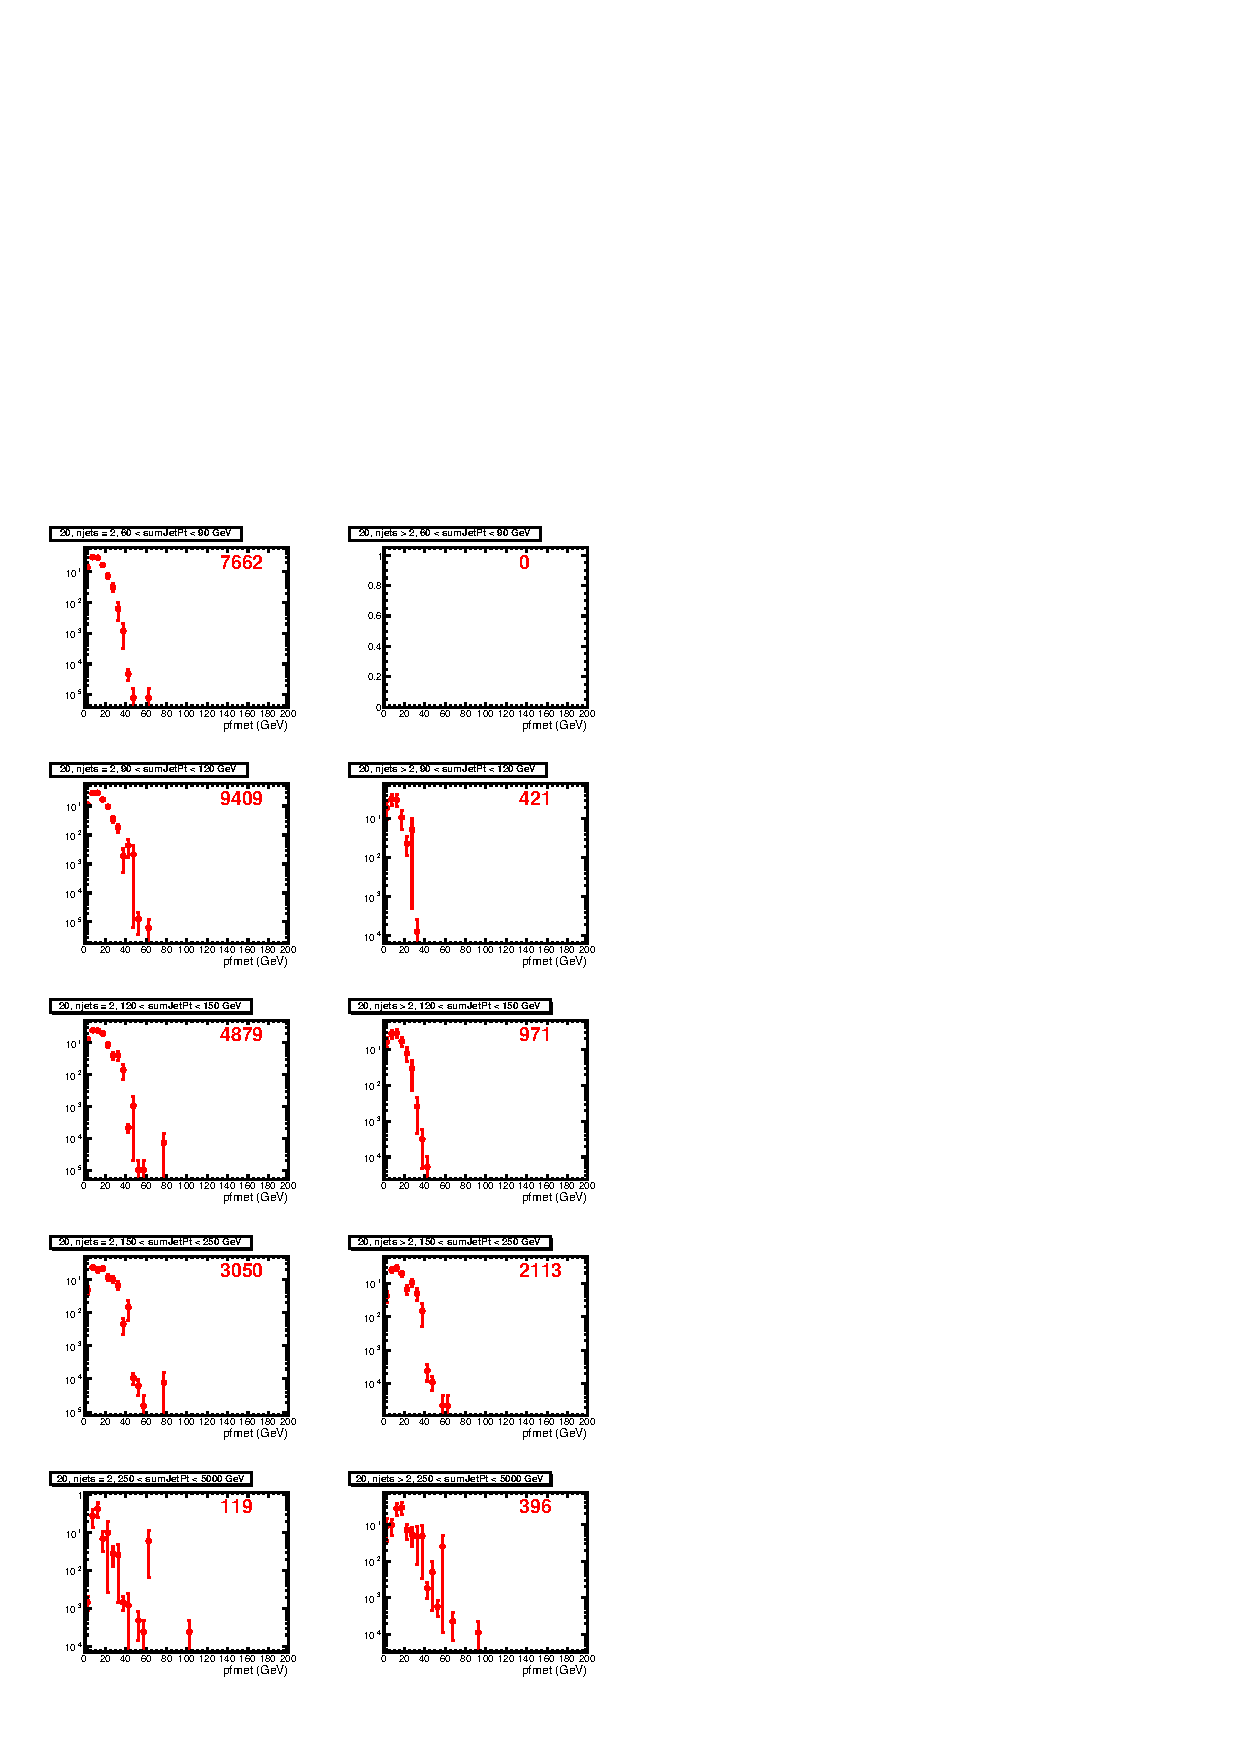
\includegraphics{plots/template_20.pdf}}
    \caption{MET Templates derived from the HLTPhoton20 sample.}
    \label{fig:template20}
  \end{center}
\end{figure}

\begin{figure}[hbt]
  \begin{center}
    \resizebox{0.7\linewidth}{!}{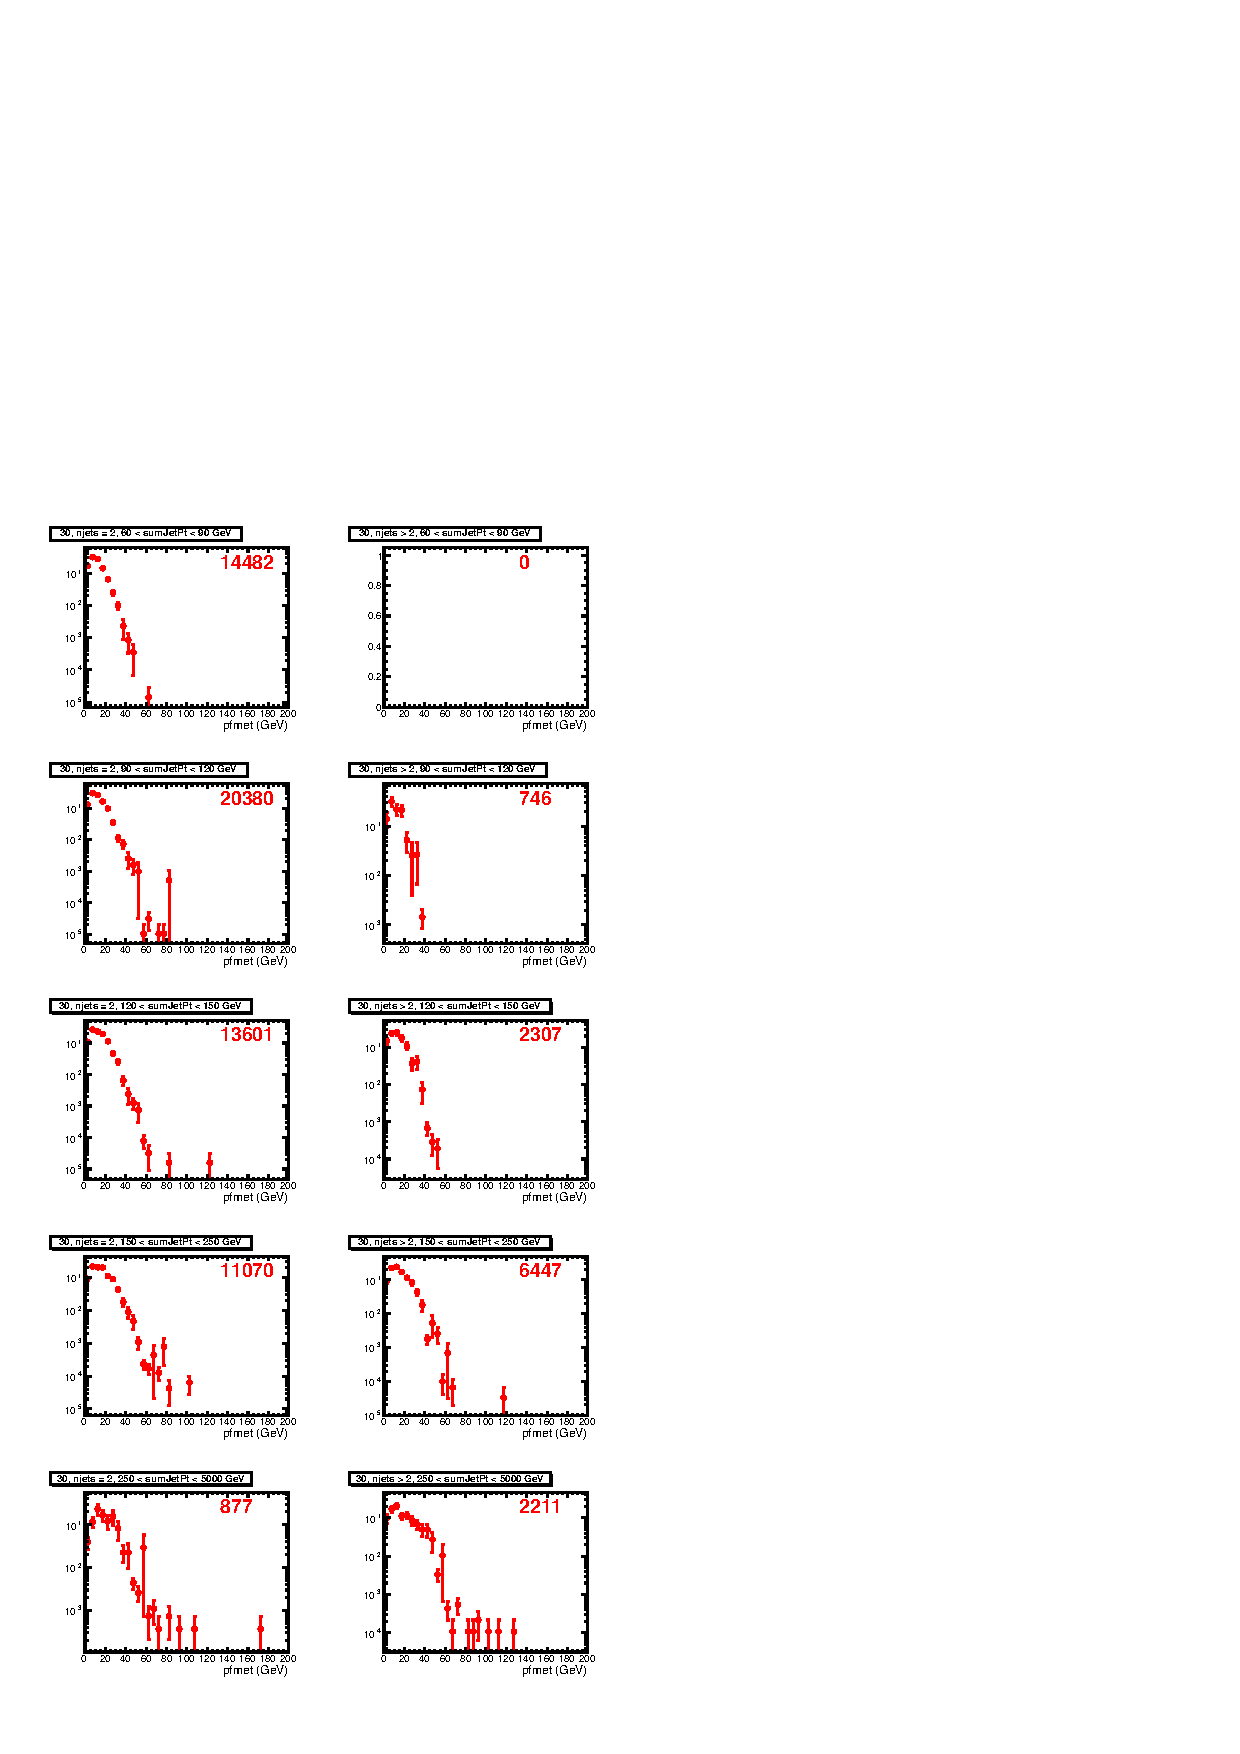
\includegraphics{plots/template_30.pdf}}
    \caption{MET Templates derived from the HLTPhoton30 sample.}
    \label{fig:template30}
  \end{center}
\end{figure}

\begin{figure}[hbt]
  \begin{center}
    \resizebox{0.7\linewidth}{!}{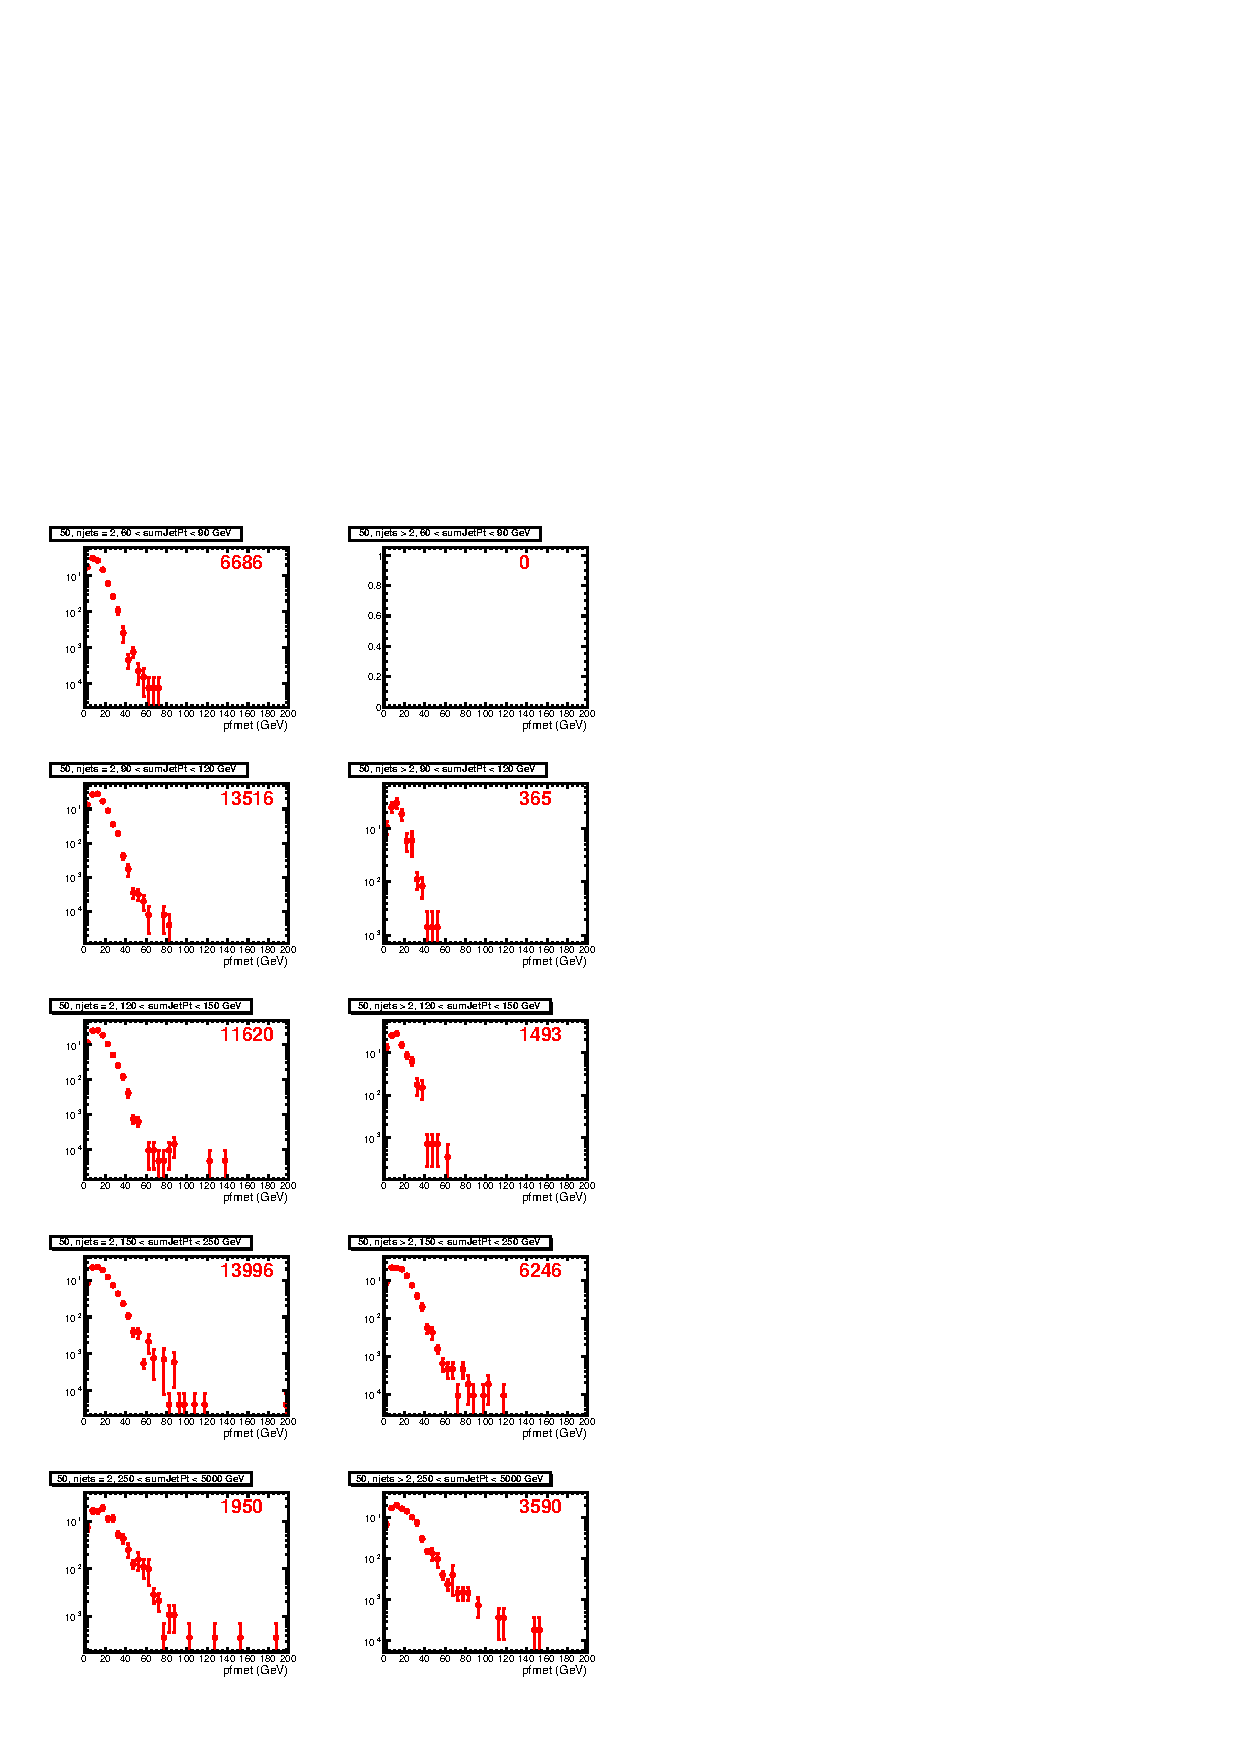
\includegraphics{plots/template_50.pdf}}
    \caption{MET Templates derived from the HLTPhoton50 sample.}
    \label{fig:template50}
  \end{center}
\end{figure}

\begin{figure}[hbt]
  \begin{center}
    \resizebox{0.7\linewidth}{!}{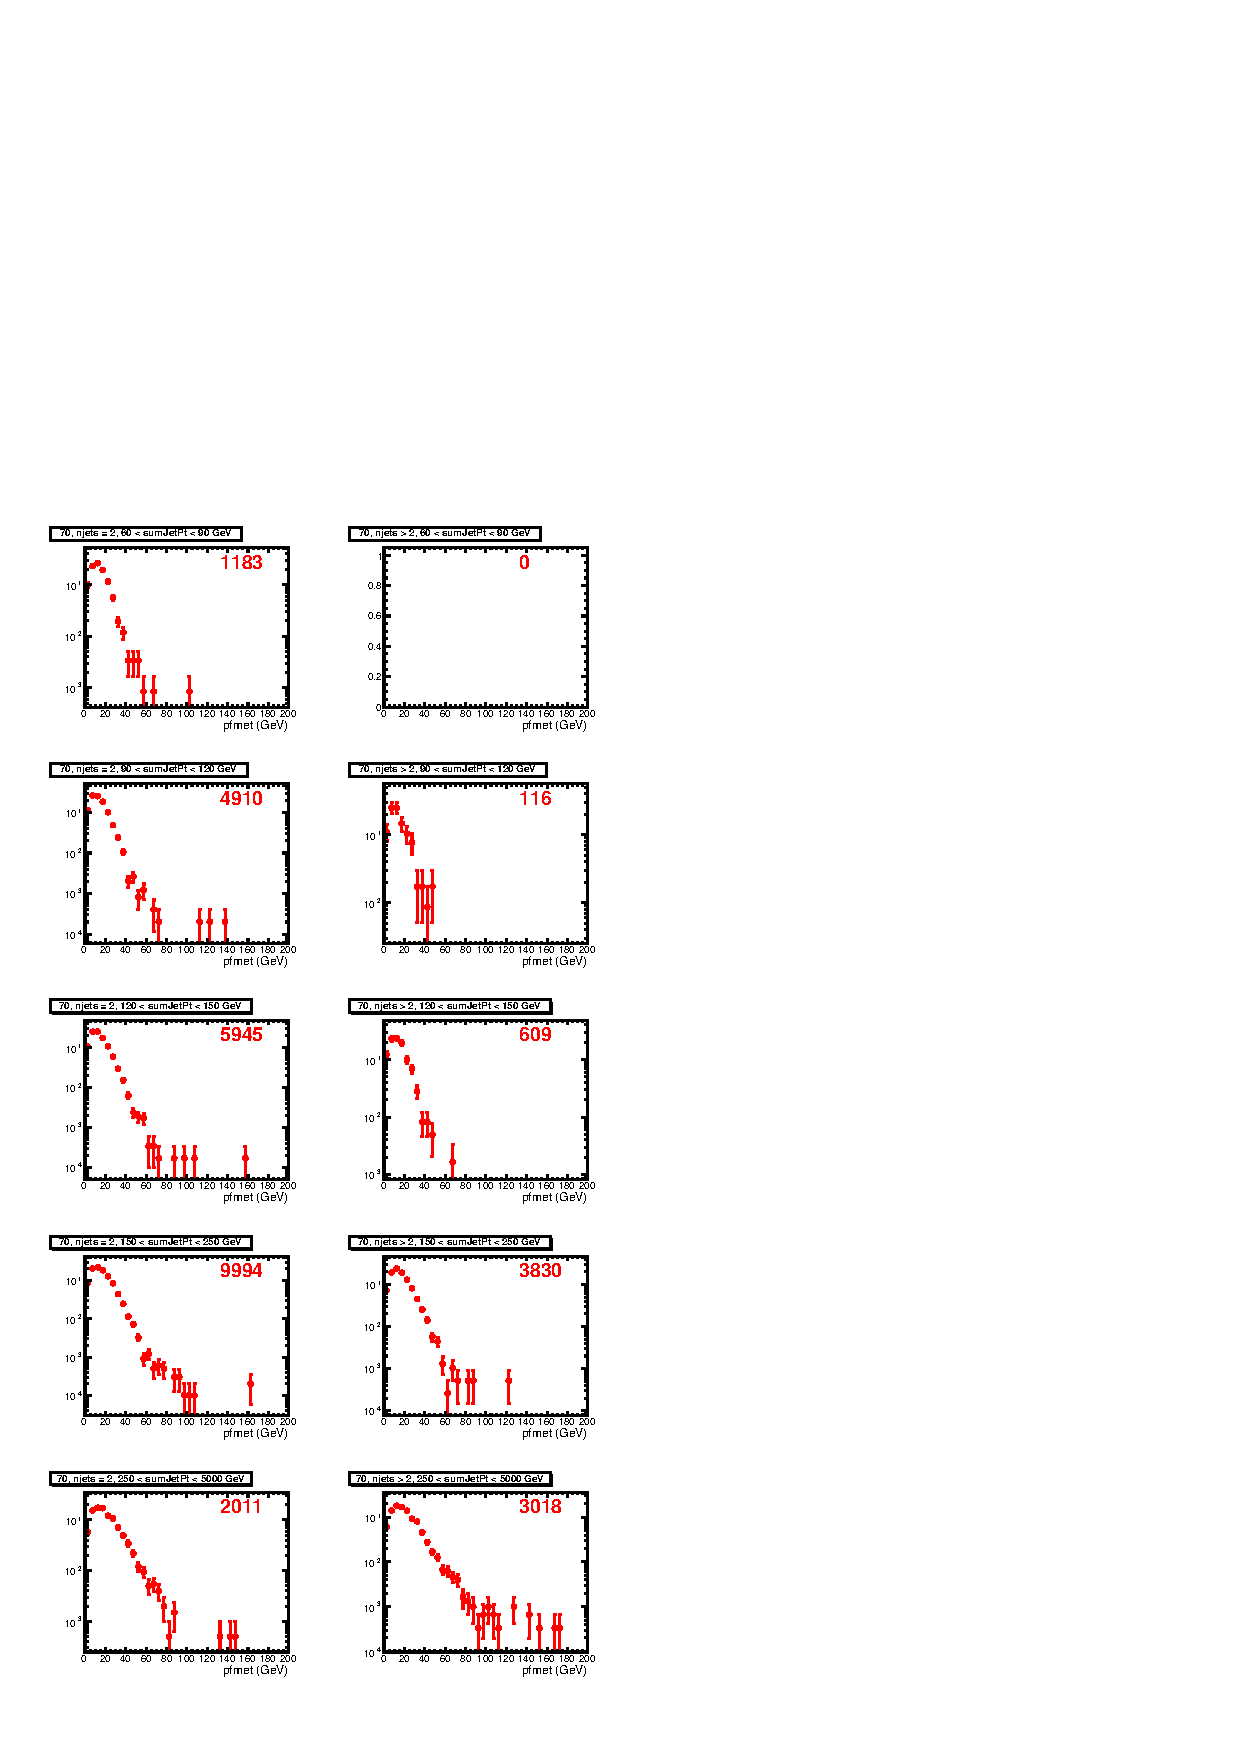
\includegraphics{plots/template_70.pdf}}
    \caption{MET Templates derived from the HLTPhoton70 sample.}
    \label{fig:template70}
  \end{center}
\end{figure}



\end{document}



